%  Work by David I. Spivak and Patrick Schultz
%
%  Creative Commons license.
%
%  Use at your own risk. 

\documentclass[11pt,oneside,article]{memoir}

\usepackage{amsthm}
\usepackage{stmaryrd}
\usepackage{newpxtext}
\usepackage[varg,bigdelims]{newpxmath}
\usepackage[usenames,dvipsnames]{xcolor}
\usepackage{tikz}

\usetikzlibrary{
	cd,
	math,
	backgrounds,
	decorations.markings,
	decorations.pathreplacing,
	positioning,
	arrows.meta,
	circuits.logic.US,
	shapes,
	calc,
	fit,
	trees,
	quotes}

\newcommand{\tn}{\textnormal}
\newcommand{\inp}[1]{#1^{\tn{in}}}
\newcommand{\outp}[1]{#1^{\tn{out}}}
\newcommand{\upd}[1]{#1^{\tn{upd}}}
\newcommand{\rdt}[1]{#1^{\tn{rdt}}}


\tikzset{
  WD/.style={%everything after equals replaces "oriented WD" in key.
  	label/.style={
    	font=\everymath\expandafter{\the\everymath\scriptstyle},
      inner sep=0pt,
      node distance=2pt and -2pt},
  	label distance=-2pt,
  	every to/.style={draw},
    semithick,
    node distance=\bbx and \bby,
    decoration={markings, mark=at position \stringdecpos with \stringdec},
    bb port length=3pt,
  	bb port sep=1,
		bb inside color=white,
		bb outside color=black,
	 	bbx = .4cm,
		bb min width=.4cm,
	  bby = 2ex,
	  bb penetrate=0,
	  bb rounded corners=2pt,
	  dot size=3pt,
    shell size = 16pt,
   	penetration = 0pt,
    link size = 2pt,
    shell color = blue,
  	shell inside color=\pcolor!20,
 	  shell outside color=\pcolor!50!black,
  	surround sep=2pt,
    ar/.style={postaction={decorate}},
  	execute at begin picture={\tikzset{
  		x=\bbx, y=\bby, 
			circuit logic US, tiny circuit symbols
			}
		}
  },
  beamer/.style={
  	bbx=.4cm,
		bb min width=.4cm,
		bby=6pt,
		bb port length=3pt,
		bb port sep=.5,
  	dot size=1pt,
    shell size = 11pt, %May look big, but this keeps fonts from mattering.
   	penetration = 0pt,
    link size = 1pt,
    shell color = blue,
    surround sep=1pt,
    inner sep=1pt,
    font=\tiny,
    bb inside color=\picolor,
    bb outside color=\pocolor,
	},
	bb standard colors/.style={bb inside color=white, bb outside color=black},
	bb inside color/.store in=\bbicolor,
	bb outside color/.store in=\bbocolor,
  bbx/.store in=\bbx,
  bby/.store in=\bby,
  bb port sep/.store in=\bbportsep,
  bb port length/.store in=\bbportlen,
  bb penetrate/.store in=\bbpenetrate,
  bb min width/.store in=\bbminwidth,
  bb rounded corners/.store in=\bbcorners,
  bb/.code 2 args={%When you see this key, run the code below:
    \pgfmathsetlengthmacro{\bbheight}{\bbportsep * (max(#1,#2)+1) * \bby}
    \pgfkeysalso{
      draw=\bbocolor,
      fill=\bbicolor,
      minimum height=\bbheight,
      minimum width=\bbminwidth,
      outer sep=0pt,
      rounded corners=\bbcorners,
      thick,
      prefix after command={\pgfextra{\let\fixname\tikzlastnode}},
      append after command={\pgfextra{\draw
      	\ifnum #1=0{} \else foreach \i in {1,...,#1} {
        	($(\fixname.north west)!{(2*\i-1)/(2*#1)}!(\fixname.south west)$) +(-\bbportlen,0) coordinate (\fixname_in\i) -- +(\bbpenetrate,0) coordinate (\fixname_in\i')}\fi 
  					%Define the endpoints of tickmarks
        \ifnum #2=0{} \else foreach \i in {1,...,#2} {
        	($(\fixname.north east)!{(2*\i-1)/(2*#2)}!(\fixname.south east)$) +(-
\bbpenetrate,0) coordinate (\fixname_out\i') -- +(\bbportlen,0) coordinate (\fixname_out\i)}\fi;
       }}}
		},
	dot size/.store in=\dotsize,
	dot/.style={
		circle, draw, thick, inner sep=0, fill=black, minimum width=\dotsize
	},
	bb name/.style={
    append after command={
		\pgfextra{\node[anchor=north] at (\fixname.north) {#1};}
		}
	},
  shell size/.store in=\psize,
	penetration/.store in=\penetration,
  spacing/.store in=\spacing,
  link size/.store in=\lsize,
  shell color/.store in=\pcolor,
 	shell inside color/.store in=\picolor,
 	shell outside color/.store in=\pocolor,
 	surround sep/.store in=\ssep,
 	link/.style={
  	circle, 
  	draw=black, 
  	fill=black,
  	inner sep=0pt, 
 		minimum size=\lsize
 	},
  shell/.style={
 		circle, 
 		draw = \pocolor, 
  	fill = \picolor,
  	minimum size = \psize
  },
  func/.style={
  	shell,
		rectangle,
		rounded corners=.5*\psize,
		inner ysep=.125*\psize,
		minimum width=1.125*\psize,
		inner xsep=.25*\psize,
  },
  funcr/.style={
    func,
    rectangle round north west=false, 
		rectangle round south west=false,
  },
  funcl/.style={
    func,
		rectangle round north east=false, 
		rectangle round south east=false,
  },
  funcu/.style={
    func,
		rectangle round south east=false, 
		rectangle round south west=false,
  },
  funcd/.style={
    func,
		rectangle round north east=false, 
		rectangle round north west=false,
  },
  outer shell/.style={
 		ellipse, 
 		draw,
  	inner sep=\ssep,
  	color=gray,
 	},
  intermediate shell/.style={
 		ellipse,
 		dashed, 
  	draw,
  	inner sep=\ssep,
 		color=\pocolor,
 	},
 }

\tikzset{
	oriented WD/.style={%everything after equals replaces "oriented WD" in key.
		every to/.style={out=0,in=180,draw},
    label/.style={
    	font=\everymath\expandafter{\the\everymath\scriptstyle},
      inner sep=0pt,
      node distance=2pt and -2pt},
    semithick,
    node distance=1 and 1,
    decoration={markings, mark=at position \stringdecpos with \stringdec},
    ar/.style={postaction={decorate}},
    execute at begin picture={\tikzset{
    	x=\bbx, y=\bby,
      every fit/.style={inner xsep=\bbx, inner ysep=\bby}}}
    },
    string decoration/.store in=\stringdec,
    string decoration={\arrow{stealth};},
    string decoration pos/.store in=\stringdecpos,
    string decoration pos=.7,
    bbx/.store in=\bbx,
    bbx = 1.5cm,
    bby/.store in=\bby,
    bby = 1.5ex,
    bb port sep/.store in=\bbportsep,
    bb port sep=1.5,
    % bb wire sep/.store in=\bbwiresep,
    % bb wire sep=1.75ex,
    bb port length/.store in=\bbportlen,
    bb port length=4pt,
    bb penetrate/.store in=\bbpenetrate,
    bb penetrate=0,
    bb min width/.store in=\bbminwidth,
    bb min width=1cm,
    bb rounded corners/.store in=\bbcorners,
    bb rounded corners=2pt,
    bb spider/.style={
    	bb port sep=1, bb port length=10pt, bbx=.4cm, bb min width=.4cm, bby=.8ex},
    bb small/.style={
    	bb port sep=1, bb port length=2.5pt, bbx=.4cm, bb min width=.4cm, bby=.7ex},
		bb medium/.style={
			bb port sep=1, bb port length=2.5pt, bbx=.4cm, bb min width=.4cm, bby=.9ex},
    bb/.code 2 args={%When you see this key, run the code below:
    	\pgfmathsetlengthmacro{\bbheight}{\bbportsep * (max(#1,#2)+1) * \bby}
      \pgfkeysalso{draw,minimum height=\bbheight,minimum
       width=\bbminwidth,outer sep=0pt,
         rounded corners=\bbcorners,thick,
         prefix after command={\pgfextra{\let\fixname\tikzlastnode}},
         append after command={\pgfextra{\draw
            \ifnum #1=0{} \else foreach \i in {1,...,#1} {
            	($(\fixname.north west)!{\i/(#1+1)}!(\fixname.south west)$) +(-\bbportlen,0) coordinate (\fixname_in\i) -- +(\bbpenetrate,0) coordinate (\fixname_in\i')}\fi 
  					%Define the endpoints of tickmarks
            \ifnum #2=0{} \else foreach \i in {1,...,#2} {
            	($(\fixname.north east)!{\i/(#2+1)}!(\fixname.south east)$) +(-
\bbpenetrate,0) coordinate (\fixname_out\i') -- +(\bbportlen,0) coordinate (\fixname_out\i)}\fi;
           }}}
		},
			bb name/.style={
     	append after command={
				\pgfextra{\node[anchor=north] at (\fixname.north) {#1};}
			}
		}
  }


  \tikzset{
  	unoriented WD/.style={
  		every to/.style={draw},
  		shorten <=-\penetration, shorten >=-\penetration,
  		label distance=-2pt,
  		thick,
  		node distance=\spacing,
  		execute at begin picture={\tikzset{
  			x=\spacing, y=\spacing}}
  		},
  	pack size/.store in=\psize,
  	pack size = 8pt,
  	spacing/.store in=\spacing,
  	spacing = 8pt,
  	link size/.store in=\lsize,
  	link size = 2pt,
		penetration/.store in=\penetration,
		penetration = 2pt,
  	pack color/.store in=\pcolor,
  	pack color = blue,
  	pack inside color/.store in=\picolor,
  	pack inside color=blue!20,
  	pack outside color/.store in=\pocolor,
  	pack outside color=blue!50!black,
  	surround sep/.store in=\ssep,
  	surround sep=8pt,
  	link/.style={
  		circle, 
  		draw=black, 
  		fill=black,
  		inner sep=0pt, 
  		minimum size=\lsize
  	},
  	pack/.style={
  		circle, 
  		draw = \pocolor, 
  		fill = \picolor,
  		inner sep = .25*\psize,
  		minimum size = \psize
  	},
  	outer pack/.style={
  		ellipse, 
  		draw,
  		inner sep=\ssep,
  		color=\pocolor,
  	},
  	intermediate pack/.style={
  		ellipse,
  		dashed, 
  		draw,
  		inner sep=\ssep,
  		color=\pocolor,
  	},
  }

\tikzset{
	spider diagram/.style={
		every to/.style={out=0, in=180, draw, thick},
		thick
	},
	dot size/.store in=\dotsize,
	dot size = 5pt,
	dot fill/.store in=\dotfill,
	dot fill = black,
	leg length/.store in=\leglen,
	leg length = 15pt,
	baby/.style={dot size = 2pt, leg length = 6pt},
	young/.style={dot size = 3pt, leg length = 10pt},
	special spider/.code n args={4}{
		\pgfkeysalso{circle, draw, thick, inner sep=0, fill=\dotfill, minimum width=\dotsize,
  		prefix after command={\pgfextra{\let\fixname\tikzlastnode}},
  		append after command={\pgfextra{
  			\ifnum #1=0{} \else {\foreach \i in {1,...,#1} {
					\tikzmath{\anglei={-90*(#1+1-2*\i)/#1};}
  				\draw [thick]
						(\fixname) .. controls 
						($(\fixname.center)-(\anglei:#3/3)$) and ($(\fixname.center)-(\anglei:#3*2/3)$) .. 
						({$(\fixname)-(\anglei:#3*2/3)$}-|{$(\fixname)-(#3,0)$}) coordinate (\fixname_in\i);
  			}}\fi
  			\ifnum #2=0{} \else {\foreach \i in {1,...,#2} {
					\tikzmath{\anglei={90*(#2+1-2*\i)/#2};}
  				\draw [thick]
						(\fixname.center) .. controls 
						($(\fixname.center)+(\anglei:#4/3)$) and ($(\fixname.center)+(\anglei:#4*2/3)$) .. 
						({$(\fixname.center)+(\anglei:#4*2/3)$}-|{$(\fixname.center)+(#4,0)$}) coordinate (\fixname_out\i);
  			}}\fi
  		}}
		}
	},
	spider/.code 2 args={
		\pgfkeysalso{special spider={#1}{#2}{\leglen}{\leglen}}
	}
}

\tikzset{Yonepart/.pic={
	\node[bb={1}{2},bb name = {\tiny$X_{11}$}] (X11) {};
	\node[bb={2}{2},below right=of X11,bb name = {\tiny$X_{12}$}] (X12) {};
	\node[bb={2}{1}, above right=of X12,bb name = {\tiny$X_{13}$}] (X13) {};
	\node[bb={2}{2}, fit={($(X11.north west)+(.3,1.5)$) (X12)  ($(X13.east)+(-.3,0)$)},bb name = {\scriptsize $Y_1$}] (Y1) {};
	\draw (Y1_in1') to (X11_in1);	
	\draw (Y1_in2') to (X12_in2);
	\draw (X11_out1) to (X13_in1);
	\draw (X11_out2) to (X12_in1);
	\draw (X12_out1) to (X13_in2);
	\draw (X12_out2) to (Y1_out2');
	\draw (X13_out1) to (Y1_out1');
	\coordinate (bottombox) at ($(X12.south)$);
	\coordinate (rightbox) at ($(X13.east)$);
	\coordinate (Y1northwest) at ($(Y1.north west)$);
	}
}

\tikzset{Ytwopart/.pic={
	\node[bb={2}{2}, bb name = {\tiny$X_{21}$}] (X21) {};
	\node[bb={1}{2},above right=-1 and 1 of X21,bb name = {\tiny$X_{22}$}] (X22) {};
	\node[bb={1}{2}, fit={($(X21.south west)+(-.25,0)$) ($(X22.north east)+(.25,3.5)$)},bb name = {\scriptsize$Y_2$}] (Y2){};
	\draw (Y2_in1') to (X21_in2);
	\draw (X21_out1) to (X22_in1);
	\draw (X22_out2) to (Y2_out1');
	\draw let \p1=(X22.south east), \p2=($(Y2_out2)$), \n1={\y1-\bby}, \n2=\bbportlen in
	  (X21_out2) to (\x1+\n2,\n1) -- (\x1+\n2,\n1) to (Y2_out2');
	\draw let \p1=(X22.north east), \p2=(X21.north west), \n1={\y1+\bby}, \n2=\bbportlen in
          (X22_out1) to[in=0] (\x1+\n2,\n1) -- (\x2-\n2,\n1) to[out=180] (X21_in1);
          }
}

\tikzset{SmallNeuronPic/.pic={
 \node[bb={3}{1}] (N1) {$\scriptstyle N_1$};
  \node[bb={2}{1}, above right=.7 and 3.5 of N1] (N2) {$\scriptstyle N_2$};
  \node[bb={2}{1}, below =of N2] (N3) {$\scriptstyle N_3$};
  \node[bb={3}{1}, below =of N3] (N4) {$\scriptstyle N_4$};
  \node[bb={6}{8}, fit={($(N1.west)-(.5,0)$) ($(N2.north)+(0,2)$) ($(N3.east)+(1.5,0)$) ($(N4.south)-(0,1)$)}, bb name={$\scriptstyle X$}] (X) {};
  \draw (X_in1') to (N2_in1);
  \draw (X_in2') to (N1_in1);
  \draw (X_in3') to (N1_in2);
  \draw (X_in4') to (N1_in3);
  \draw (X_in6') to (N4_in2);
  \draw (N1_out1) to (N2_in2);
  \draw (N1_out1) to (N3_in1);
  \draw (N1_out1) to (N4_in1);
  \draw (N2_out1) to (X_out1');
  \draw (N2_out1) to (X_out2');
  \draw (N2_out1) to (X_out3');
  \draw (N3_out1) to (X_out4');
  \draw (N3_out1) to (X_out5');
  \draw (N3_out1) to (X_out6');
  \draw (N4_out1) to (X_out7');
  \draw (N4_out1) to (X_out8'); 
  \draw (X_in5') to[looseness=2] (N3_in2);
  \draw let \p1=(N4.south east), \p2=(N4.south west), \n1={\y2-\bby}, \n2=\bbportlen in
          (N3_out1) to[in=0] (\x1+\n2,\n1) -- (\x2-\n2,\n1) to[out=180] (N4_in3);
}
}

\tikzset{SmallNeuronDashed/.pic={
 \node[bb={3}{1}] (N1) {$\scriptstyle N_1$};
  \node[bb={2}{1}, above right=.7 and 3.5 of N1] (N2) {$\scriptstyle N_2$};
  \node[bb={2}{1}, below =of N2] (N3) {$\scriptstyle N_3$};
  \node[bb={3}{1}, below =of N3] (N4) {$\scriptstyle N_4$};
  \node[bb={6}{8}, fit={($(N1.west)-(.5,0)$) ($(N2.north)+(0,2)$) ($(N3.east)+(1.5,0)$) ($(N4.south)-(0,1)$)}, bb name={$\scriptstyle X$}] (X) {};
  \draw[dashed] (X_in1') to (N2_in1);
  \draw[dashed] (X_in2') to (N1_in1);
  \draw[dashed] (X_in3') to (N1_in2);
  \draw[dashed] (X_in4') to (N1_in3);
  \draw[dashed] (X_in6') to (N4_in2);
  \draw[dashed] (N1_out1) to (N2_in2);
  \draw[dashed] (N1_out1) to (N3_in1);
  \draw[dashed] (N1_out1) to (N4_in1);
  \draw[dashed] (N2_out1) to (X_out1');
  \draw[dashed] (N2_out1) to (X_out2');
  \draw[dashed] (N2_out1) to (X_out3');
  \draw[dashed] (N3_out1) to (X_out4');
  \draw[dashed] (N3_out1) to (X_out5');
  \draw[dashed] (N3_out1) to (X_out6');
  \draw[dashed] (N4_out1) to (X_out7');
  \draw[dashed] (N4_out1) to (X_out8'); 
  \draw[dashed] (X_in5') to[looseness=2] (N3_in2);
  \draw[dashed] let \p1=(N4.south east), \p2=(N4.south west), \n1={\y2-\bby}, \n2=\bbportlen in
          (N3_out1) to[in=0] (\x1+\n2,\n1) -- (\x2-\n2,\n1) to[out=180] (N4_in3);
}
}

\tikzset{SmallNestingPic/.pic={
\path (0,0) pic [purple] {Yonepart};
\path ($(rightbox)+(5,-5)$) pic [orange] {Ytwopart};
 
\node[bb={1}{2}, fit={($(Y1northwest)+(-.5,4)$) ($(Y2.south east)+(1,0)$)}, bb name={\small $Z$}] (Z) {};
\draw (Z_in1') to (Y1_in2);
\draw let \p1=(Y2.north west),\p2=(Y2.north east),\n1={\y2+\bby},\n2=\bbportlen in
  (Y1_out1) to (\x1+\n2,\n1)--(\x2+\n2,\n1) to (Z_out1');
\draw (Y1_out2) to (Y2_in1);
\draw (Y2_out2) to (Z_out2');
\draw let \p1=(Y2.north east), \p2=(Y1.north west), \n1={\y2+\bby}, \n2=\bbportlen in
          (Y2_out1) to[in=0] (\x1+\n2,\n1) -- (\x2-\n2,\n1) to[out=180] (Y1_in1);
          }
}


\tikzset{Zredgreen/.pic={
\node[bb={2}{2}, green!50!black, bb name = $\scriptstyle Y_1$] (YY1) {};
\node[bb={1}{2}, red, below right=-1 and 2 of YY1, bb name=$\scriptstyle Y_2$] (YY2) {};
\node[bb={1}{2}, fit={($(YY1.north west)+(-.5,4)$) ($(YY2.south east)+(.5,-2)$)}, bb name={\scriptsize $Z$}] (Z) {};
\draw (Z_in1') to (YY1_in2);
\draw (YY1_out1) to (Z_out1');
\draw (YY1_out2) to (YY2_in1);
\draw (YY2_out2) to (Z_out2');
\draw let \p1=(YY2.north east), \p2=(YY1.north west), \n1={\y2+\bby}, \n2=\bbportlen in
          (YY2_out1) to[in=0] (\x1+\n2,\n1) -- (\x2-\n2,\n1) to[out=180] (YY1_in1);
}
}

\tikzset{Zcombined/.pic={
	\node[bb={1}{2},green!25!black,bb name = {\tiny$X_{11}$}] (X11) {};
	\node[bb={2}{2},green!25!black,below right=of X11,bb name = {\tiny$X_{12}$}] (X12) {};
	\node[bb={2}{1}, green!25!black,above right=of X12,bb name = {\tiny$X_{13}$}] (X13) {};
	\draw (X11_out1) to (X13_in1);
	\draw (X11_out2) to (X12_in1);
	\draw (X12_out1) to (X13_in2);

	\node[bb={2}{2}, red!30!black, below right = 0 and 1.25 of X12, bb name = {\tiny$X_{21}$}] (X21) {};
	\node[bb={1}{2}, red!30!black, above right=-1 and 1 of X21,bb name = {\tiny$X_{22}$}] (X22) {};
	\draw (X21_out1) to (X22_in1);
	\draw let \p1=(X22.north east), \p2=(X21.north west), \n1={\y1+\bby}, \n2=\bbportlen in
          (X22_out1) to[in=0] (\x1+\n2,\n1) -- (\x2-\n2,\n1) to[out=180] (X21_in1);
        
        \node[bb={1}{2}, fit = {($(X11.north east)+(-1,3)$) (X12) (X13) ($(X21.south)+(0,-1)$) ($(X22.east)+(.5,0)$)}, bb name ={\scriptsize $Z$}] (Z) {};
	
	\draw (Z_in1') to (X12_in2);
	\draw (X13_out1) to (Z_out1');
	\draw (X12_out2) to (X21_in2);
	\draw let \p1=(X22.south east),\n1={\y1-\bby}, \n2=\bbportlen in
	  (X21_out2) to (\x1+\n2,\n1) to (Z_out2');
	\draw let \p1=(X22.north east), \p2=(X11.north west), \n1={\y2+\bby}, \n2=\bbportlen in
          (X22_out2) to[in=0] (\x1+\n2,\n1) -- (\x2-\n2,\n1) to[out=180] (X11_in1);
}
}


\settrims{0pt}{0pt} % page and stock same size
%\setlxvchars %calculate line length such that there are about 65 characters per line in \normalfont
\settypeblocksize{*}{35pc}{*} % {height}{width}{ratio}
%\settypeblocksize{*}{39pc}{*} % {height}{width}{ratio}
\setlrmargins{*}{*}{1} % {spine}{edge}{ratio}
%\setulmargins{*}{*}{1} % {upper}{lower}{ratio}, hight of typeblock fixed
\setulmarginsandblock{1in}{1in}{*} % height of typeblock computed
\setheadfoot{\onelineskip}{2\onelineskip} % {headheight}{footskip}
\setheaderspaces{*}{1.5\onelineskip}{*} % {headdrop}{headsep}{ratio}
\checkandfixthelayout

\setcounter{tocdepth}{1}
\setcounter{secnumdepth}{1}
\pagestyle{ruled}
\renewcommand*{\chaptitlefont}{\bfseries\Large}
\setsecheadstyle{\bfseries\large\raggedright}
\setsubsecheadstyle{\bfseries\raggedright}


\begin{document}

\title{Collected Wiring diagrams}
\author{David I. Spivak}

\maketitle


\begin{equation}\label{eqn.overview}\tag{overview}
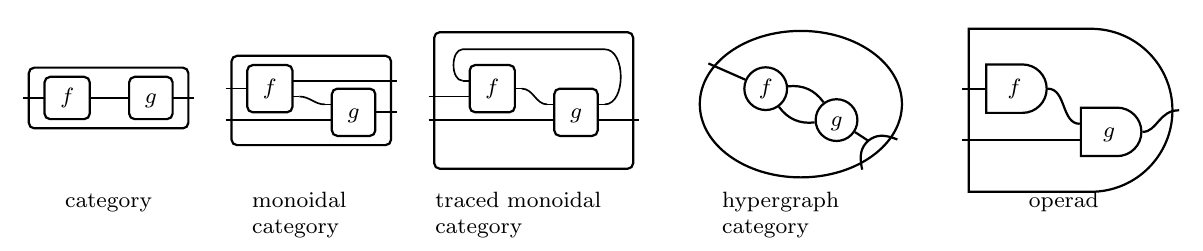
\begin{tikzpicture}
\begin{scope}[font=\footnotesize, text height=1.5ex, text depth=.5ex]
  \begin{scope}[oriented WD, bb port sep=1, bb port length=2.5pt, bb min width=.4cm, bby=.2cm, inner xsep=.2cm, x=.5cm, y=.3cm]
  	\node[bb={1}{1}] (Catf) {$f$};
  	\node[bb={1}{1}, right=1 of Catf] (Catg) {$g$};
  	\node[bb={0}{0}, fit=(Catf) (Catg)] (Cat) {};
  	\node[coordinate] at (Cat.west|-Catf_in1) (Cat_in1) {};
  	\node[coordinate] at (Cat.east|-Catg_out1) (Cat_out1) {};
  	\draw[shorten <=-2pt] (Cat_in1) -- (Catf_in1);
  	\draw (Catf_out1) -- (Catg_in1);
  	\draw[shorten >=-2pt] (Catg_out1) -- (Cat_out1);
  %
  	\node[bb={1}{2}, above right=-1.5 and 4 of Catf] (Monf) {$f$};
  	\node[bb={2}{1}, below right=-1 and 1 of Monf] (Mong) {$g$};
  	\node[bb={0}{0}, fit=(Monf) (Mong)] (Mon) {};
  	\node[coordinate] at (Mon.west|-Monf_in1) (Mon_in1) {};
  	\node[coordinate] at (Mon.west|-Mong_in2) (Mon_in2) {};
  	\node[coordinate] at (Mon.east|-Monf_out1) (Mon_out1) {};
  	\node[coordinate] at (Mon.east|-Mong_out1) (Mon_out2) {};
  	\draw[shorten <=-2pt] (Mon_in1) -- (Monf_in1);
  	\draw[shorten >=-2pt] (Monf_out1) -- (Mon_out1);
  	\draw (Monf_out2) to (Mong_in1);
  	\draw[shorten <=-2pt] (Mon_in2) -- (Mong_in2);
  	\draw[shorten >=-2pt] (Mong_out1) -- (Mon_out2);
  %
  	\node[bb={2}{1}, right= 4.5 of Monf] (Trf) {$f$};
  	\node[bb={2}{2}, below right=-1 and 1 of Trf] (Trg) {$g$};
  	\node[bb={0}{0}, fit={($(Trf.north west)+(-.5,1)$) ($(Trg.south east)+(.5,-1)$)}] (Tr) {};
  	\node[coordinate] at (Tr.west|-Trf_in2) (Tr_in1) {};
  	\node[coordinate] at (Tr.west|-Trg_in2) (Tr_in2) {};
  	\node[coordinate] at (Tr.east|-Trf_out1) (Tr_out1) {};
  	\node[coordinate] at (Tr.east|-Trg_out2) (Tr_out2) {};
  	\draw[shorten <=-2pt] (Tr_in1) -- (Trf_in2);
  	\draw (Trf_out1) to (Trg_in1);
  	\draw[shorten <=-2pt] (Tr_in2) -- (Trg_in2);
  	\draw[shorten >=-2pt] (Trg_out2) -- (Tr_out2);
  	\draw let \p1=(Trg.east), \p2=(Trf.north west), \n1=\bbportlen, \n2=\bby in
  		(Trg_out1) to[in=0] (\x1+\n1,\y2+\n2) -- (\x2-\n1,\y2+\n2) to[out=180] (Trf_in1);
  %
  \end{scope}
  \begin{scope}[penetration=0, unoriented WD, pack outside color=black, pack inside color=white]
  	\node[pack, right=2.9 of Trf] (Hypf) {$f$};
  	\node[pack, below right=0 and .5 of Hypf] (Hypg) {$g$};
  	\node[outer pack, inner sep=5pt, fit=(Hypf) (Hypg)] (Hyp) {};
  	\node[coordinate] at ($(Hypg.-30)!.5!(Hyp.-30)$) (link) {};
  	\draw (Hypf) to[bend left] (Hypg);
  	\draw (Hypf) to[bend right] (Hypg);
  	\draw (Hypg) -- (link);
  	\draw[shorten >= -2pt] (link) to[bend left] (Hyp.-20);
  	\draw[shorten >= -2pt] (link) to[bend right] (Hyp.-45);
  	\draw[shorten >= -2pt] (Hypf) -- (Hyp);
  \end{scope}
  \begin{scope}[circuit logic US, thick, every to/.style={out=0,in=180}]
  	\node[and gate, draw, right=2.5 of Hypf] (Opdf) {$f$};
  	\node[and gate, draw, below right=0 and 0.5 of Opdf] (Opdg) {$g$};
		\node[and gate, inner sep=1pt, draw, fit=(Opdf) (Opdg)] (Opd) {};
		\draw[shorten <=-2pt] (Opd.input 1|-Opdf.west) to (Opdf.west);
		\draw[shorten <=-2pt] (Opd.input 1|-Opdg.input 2) to (Opdg.input 2);
		\draw (Opdf.output) to (Opdg.input 1);
		\draw[shorten >=-2pt] (Opdg.output) to (Opd.output);
  \end{scope}
	\node[below=.65 of Cat.south] (Cat name) {category};
	\node[text width=1.5cm] at (Cat name-|Mon) {monoidal category};
	\node[text width=2.5cm] at (Cat name-|Tr) {traced monoidal category};
	\node[text width=2cm] at (Cat name-|Hyp) {hypergraph category};
	\node at (Cat name-|Opd) {operad};
\end{scope}
\end{tikzpicture}
\end{equation}

\begin{equation}\label{eqn.overview2}\tag{overview2}
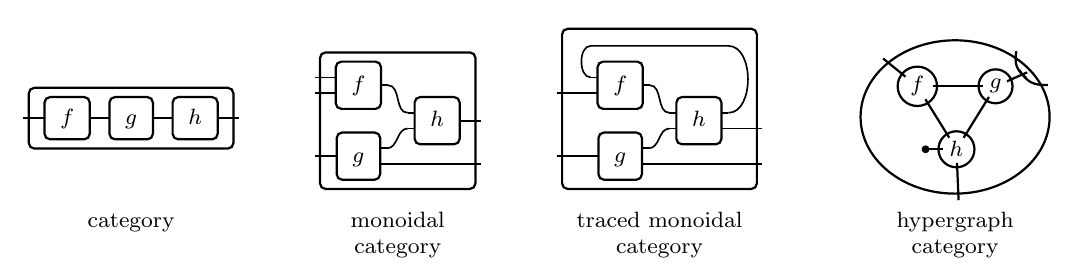
\begin{tikzpicture}
\begin{scope}[font=\footnotesize]
  \begin{scope}[oriented WD, bb port sep=1, bb port length=2.5pt, bb min width=.4cm, bby=.2cm, inner xsep=.2cm, x=.5cm, y=.3cm, text height=1.5ex, text depth=.5ex]
  	\node[bb={1}{1}] (Catf) {$f$};
  	\node[bb={1}{1}, right=.5 of Catf] (Catg) {$g$};
  	\node[bb={1}{1}, right=.5 of Catg] (Cath) {$h$};
  	\node[bb={0}{0}, fit=(Catf) (Cath)] (Cat) {};
  	\node[coordinate] at (Cat.west|-Catf_in1) (Cat_in1) {};
  	\node[coordinate] at (Cat.east|-Catg_out1) (Cat_out1) {};
  	\draw[shorten <=-2pt] (Cat_in1) -- (Catf_in1);
  	\draw (Catf_out1) -- (Catg_in1);
  	\draw (Catg_out1) -- (Cath_in1);
  	\draw[shorten >=-2pt] (Cath_out1) -- (Cat_out1);
  %
  	\node[bb={2}{1}, above right=-.5 and 3 of Cath] (Monf) {$f$};
  	\node[bb={1}{2}, below=1 of Monf] (Mong) {$g$};
		\node[bb={2}{1}] at ($(Monf)!.5!(Mong)+(2,0)$) (Monh) {$h$}; 
  	\node[bb={0}{0}, fit=(Monf) (Mong) (Monh)] (Mon) {};
  	\node[coordinate] at (Mon.west|-Monf_in1) (Mon_in1) {};
  	\node[coordinate] at (Mon.west|-Monf_in2) (Mon_in2) {};
  	\node[coordinate] at (Mon.west|-Mong_in1) (Mon_in3) {};
  	\node[coordinate] at (Mon.east|-Monh_out1) (Mon_out1) {};
  	\node[coordinate] at (Mon.east|-Mong_out2) (Mon_out2) {};
  	\draw[shorten <=-2pt] (Mon_in1) -- (Monf_in1);
  	\draw[shorten <=-2pt] (Mon_in2) -- (Monf_in2);
  	\draw[shorten <=-2pt] (Mon_in3) -- (Mong_in1);
  	\draw[shorten >=-2pt] (Monh_out1) -- (Mon_out1);
  	\draw[shorten >=-2pt] (Mong_out2) -- (Mon_out2);
		\draw (Monf_out1) to (Monh_in1);
		\draw (Mong_out1) to (Monh_in2);
  %
  	\node[bb={2}{1}, right= 5.5 of Monf] (Trf) {$f$};
  	\node[bb={1}{2}, below=1 of Trf] (Trg) {$g$};
		\node[bb={2}{2}] at ($(Trf)!.5!(Trg)+(2,0)$) (Trh) {$h$}; 
  	\node[bb={0}{0}, fit={($(Trf.north west)+(-.5,1)$) (Trg) ($(Trh.north east)+(.5,0)$)}] (Tr) {};
  	\node[coordinate] at (Tr.west|-Trf_in2) (Tr_in1) {};
  	\node[coordinate] at (Tr.west|-Trg_in1) (Tr_in2) {};
  	\node[coordinate] at (Tr.east|-Trh_out2) (Tr_out1) {};
  	\node[coordinate] at (Tr.east|-Trg_out2) (Tr_out2) {};
  	\draw[shorten <=-2pt] (Tr_in1) -- (Trf_in2);
  	\draw[shorten <=-2pt] (Tr_in2) -- (Trg_in1);
  	\draw[shorten >=-2pt] (Trh_out2) -- (Tr_out1);
  	\draw[shorten >=-2pt] (Trg_out2) -- (Tr_out2);
		\draw (Trf_out1) to (Trh_in1);
		\draw (Trg_out1) to (Trh_in2);
  	\draw let \p1=(Trh.east), \p2=(Trf.north west), \n1=\bbportlen, \n2=\bby in
  		(Trh_out1) to[in=0] (\x1+\n1,\y2+\n2) -- (\x2-\n1,\y2+\n2) to[out=180] (Trf_in1);
  \end{scope}
  \begin{scope}[unoriented WD, penetration=0, pack outside color=black, pack inside color=white, link size=2pt]
  	\node[pack, above right=-.5 and 3.3 of Trf] (Hypf) {$f$};
  	\node[pack, right=.5 of Hypf] (Hypg) {$g$};
		\node[pack] at ($(Hypf)!.5!(Hypg)+(0,-.8)$) (Hyph) {$h$};
  	\node[outer pack, inner xsep=3pt, inner ysep=1pt, fit=(Hypf) (Hypg) (Hyph)] (Hyp) {};
  	\node[coordinate] at ($(Hypg.30)!.5!(Hyp.30)$) (link1) {};
  	\node[link,  left=.1 of Hyph.west] (link2) {};
  	\draw (Hypg) -- (link1);
  	\draw[shorten >= -2pt] (link1) to[bend right] (Hyp.20);
  	\draw[shorten >= -2pt] (link1) to[bend left] (Hyp.45);
		\draw (link2) -- (Hyph);
  	\draw[shorten >= -2pt] (Hypf) -- (Hyp);
  	\draw[shorten >= -2pt] (Hyph) -- (Hyp);
		\draw (Hypf) -- (Hyph);
		\draw (Hypf) -- (Hypg);
		\draw (Hypg) -- (Hyph);
  \end{scope}
  \begin{scope}[text height=1.5ex, text depth=.5ex, align=center]
  	\node[below=.65 of Cat.south] (Cat name) {category};
  	\node[text width=1.5cm] at (Cat name-|Mon) {monoidal category};
  	\node[text width=2.5cm] at (Cat name-|Tr) {traced monoidal\\category};
  	\node[text width=2cm] at (Cat name-|Hyp) {hypergraph category};
	\end{scope}
\end{scope}
\end{tikzpicture}
\end{equation}

%%%% Chapter %%%%
\chapter{Boxes}

\begin{equation}\label{box1}\tag{box1}
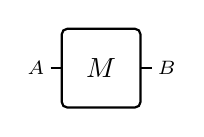
\begin{tikzpicture}[oriented WD, bbx = 1cm, bby =.5cm, bb min width=1cm, bb port length=4pt, bb port sep=1]
	\node[bb={1}{1}] (X) {$M$};
	\draw[label] 
		node [left=2pt of X_in1] {$A$}
		node [right=2pt of X_out1] {$B$}
		;
\end{tikzpicture}
\end{equation}

\begin{equation}\label{box2}\tag{box2}
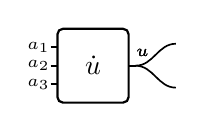
\begin{tikzpicture}[oriented WD, bb small, bb port sep=2.2, baseline = (lone.center)]
	\node[bb={3}{1}, inner sep=10pt] (lone) {$\dot{u}$};
	\node[above right=-3 and 1.5 of lone] (a) {};
	\node[below right=-3 and 1.5 of lone] (b) {};	
	\draw (lone_out1) to (a);
	\draw (lone_out1) to (b);
	\draw [label] 
		\foreach \i in {1,2,3} {
			node[anchor=east] at (lone_in\i) {\small $a_\i$}
		node[above right=1 and 0 of lone_out1] {\small $u$}
		}
	;
\end{tikzpicture}
\end{equation}

\begin{equation}\label{box3}\tag{box3}
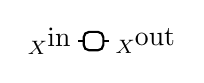
\begin{tikzpicture}[oriented WD, bbx = .25cm, bby =.1cm, bb min width=.25cm, bb port length=2pt, bb port sep=1]
	\node[bb={1}{1}] (X) {};
	\draw[label] 
		node [left=2pt of X_in1] {$\inp{X}$}
		node [right=2pt of X_out1] {$\outp{X}$}
		;
\end{tikzpicture}
\end{equation}

\begin{equation}\label{box32}\tag{box32}
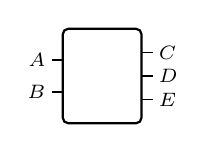
\begin{tikzpicture}[oriented WD, bbx = 1cm, bby =.3cm, bb min width=1cm, bb port length=4pt, bb port sep=1]
	\node[bb={2}{3}] (X) {};
	\draw[label] 
		node [left=2pt of X_in1] {$A$}
		node [left=2pt of X_in2] {$B$}
		node [right=2pt of X_out1] {$C$}
		node [right=2pt of X_out2] {$D$}
		node [right=2pt of X_out3] {$E$}
		;
	\end{tikzpicture}
\end{equation}

\begin{equation}\label{lots}\tag{lots}
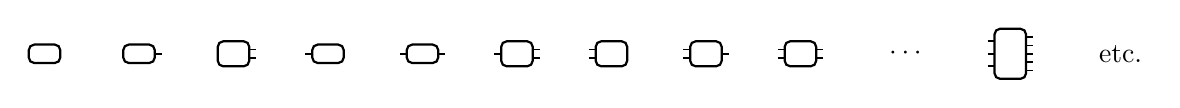
\begin{tikzpicture}[oriented WD, bb small]
	\node[bb={0}{0}]                (00) {};
	\node[bb={0}{1}, right=2 of 00] (01) {};
	\node[bb={0}{2}, right=2 of 01] (02) {};
	\node[bb={1}{0}, right=2 of 02] (10) {};
	\node[bb={1}{1}, right=2 of 10] (11) {};
	\node[bb={1}{2}, right=2 of 11] (12) {};
	\node[bb={2}{0}, right=2 of 12] (20) {};
	\node[bb={2}{1}, right=2 of 20] (21) {};	
	\node[bb={2}{2}, right=2 of 21] (22) {};
	\node[           right=2 of 22] (dt) {$\cdots$};	
	\node[bb={3}{5}, right=2 of dt] (35) {};
	\node[           right=2 of 35] (et) {etc.};	
\end{tikzpicture}
\end{equation}

%%%% Chapter %%%%
\chapter{Simple Wiring Diagrams}

\begin{equation}\label{simple3}\tag{simple 3}
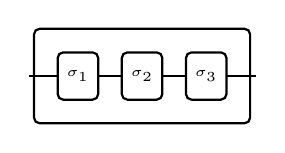
\begin{tikzpicture}[oriented WD, bbx = .3cm, bby =.3cm, bb min width=.5cm, bb port length=2pt, bb port sep=1]
	\node[bb={1}{1}] (X1) {\tiny$\sigma_1$};
  	\node[bb={1}{1}, right=of X1] (X2) {\tiny$\sigma_2$};
	\node[bb={1}{1}, right=of X2] (X3) {\tiny$\sigma_3$};
	\node[bb={1}{1}, fit=(X1) (X2) (X3)] (Y) {};
	\draw (Y_in1') to (X1_in1);
	\draw (X1_out1) to (X2_in1);
	\draw (X2_out1) to (X3_in1);
	\draw (X3_out1) to (Y_out1');
\end{tikzpicture}
\end{equation}

\begin{equation}\label{no_exterior}\tag{no exterior}
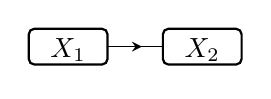
\begin{tikzpicture}[oriented WD, bbx=1em, bby=1ex]
 \node[bb={0}{1},bb name=$X_1$] (X1) {};
 \node[bb={1}{0},right =2 of X1, bb name=$X_2$] (X2) {};
 \draw[ar] (X1_out1) to (X2_in1);
\end{tikzpicture}
\end{equation}

\begin{equation}\label{simple2}\tag{simple 2}
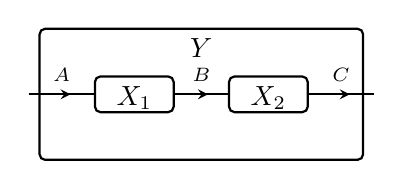
\begin{tikzpicture}[oriented WD, bbx=1em, bby=1ex]
 \node[bb={1}{1},bb name=$X_1$] (X1) {};
 \node[bb={1}{1},right =2 of X1, bb name=$X_2$] (X2) {};
 \node[bb={1}{1}, fit={($(X1.north west)+(-1,3)$) ($(X1.south)+(0,-3)$) ($(X2.east)+(1,0)$)}, bb name = $Y$] (Y) {};
%
 \draw[ar] (Y_in1') to (X1_in1);
 \draw[ar] (X1_out1) to (X2_in1);
 \draw[ar] (X2_out1) to (Y_out1');
 \draw[label] 
	node at ($(Y_in1')!.5!(X1_in1)+(0,7pt)$)  {$A$}
	node at ($(X1_out1)!.5!(X2_in1)+(0,7pt)$)   {$B$}
	node at ($(X2_out1)!.5!(Y_out1')+(0,7pt)$)  {$C$};
\end{tikzpicture}
\end{equation}

\begin{equation}\label{no_passing_wires}\tag{no passing wires}
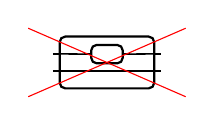
\begin{tikzpicture}[oriented WD, bb small]
		\node[bb={1}{1}] (x) {};
		\node[bb={2}{2}, fit={(x.north west) ($(x.south east)+(0,-2)$)}] (y) {};
		\draw (y_in1') to (x_in1);
		\draw (x_out1) to (y_out1');
		\draw (y_in2') to (y_out2');
		\draw[red, thin] ($(y.north west)+(-1,1)$) -- ($(y.south east)+(1,-1)$);
		\draw[red, thin] ($(y.north east)+(1,1)$) -- ($(y.south west)+(-1,-1)$);
\end{tikzpicture}
\end{equation}

\begin{equation}\label{digging1}\tag{digging1}
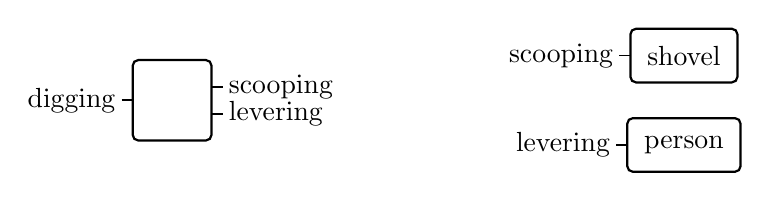
\begin{tikzpicture}[oriented WD]
	\node[bb={1}{0}] (shovel) {\;shovel\;};
	\node[bb={1}{0}, below=2 of shovel] (person) {\;person\;};
	\node[bb={1}{2}, left=4 of $(shovel)!.5!(person)$] (dig) {};

	\draw[label] 
		node [left=2pt of dig_in1] {digging}
		node [right=2pt of dig_out1] {scooping}
		node [right=2pt of dig_out2] {levering}
		node [left=2pt of shovel_in1] {scooping}
		node [left=2pt of person_in1] {levering}
		;
\end{tikzpicture}
\end{equation}

\begin{equation}\label{digging2}\tag{digging2}
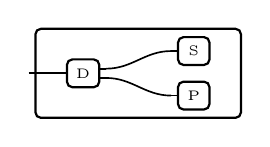
\begin{tikzpicture}[oriented WD,bb small, font=\tiny]
	\node[bb={1}{0}] (shovel) {S};
	\node[bb={1}{0}, below=2 of shovel] (person) {P};
	\node[bb={1}{2}, left=3 of $(shovel)!.5!(person)$] (dig) {D};
	\node[bb={1}{0}, fit=(dig) (shovel) (person)] (outer) {};
	\draw (outer_in1') to (dig_in1);
	\draw (dig_out1) to (shovel_in1);
	\draw (dig_out2) to (person_in1);
\end{tikzpicture}
\end{equation}

\begin{equation}\label{eqn.pop}\tag{pop}
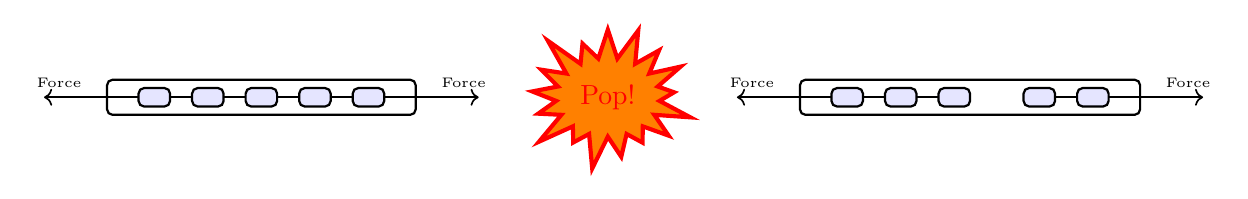
\begin{tikzpicture}[oriented WD, bb small, bb port length=0]
	\foreach \i in {0,...,4} {
		\node[bb={1}{1}, fill=blue!10] at (1.7*\i,0) (X\i) {};
	}
	\node[bb={1}{1}, fit=(X0) (X4)] (X) {};
	\foreach \i in {0,...,3} {
		\draw[thick] (X\i_out1) -- (X\the\numexpr\i+1\relax_in1);
	};
	\draw[->] (X0_in1) -- node[above left, font=\tiny] {Force} +(-3,0);
	\draw[->] (X4_out1) -- node[above right, font=\tiny] {Force} +(3,0) node (R) {};
%
\def\x{22};
	\foreach \i in {0,...,2} {
		\node[bb={1}{1}, fill=blue!10] at (\x+1.7*\i,0) (Y\i) {};
	}
	\foreach \i in {3,...,4} {
		\node[bb={1}{1}, fill=blue!10] at (\x+1+1.7*\i,0) (Y\i) {};
	}
	\node[bb={1}{1}, fit=(Y0) (Y4)] (Y) {};
	\foreach \i in {0,1,3} {
		\draw[thick] (Y\i_out1) -- (Y\the\numexpr\i+1\relax_in1);
	};
	\draw[->] (Y0_in1) -- node[above left, font=\tiny] {Force} +(-3,0) node (L) {};
	\draw[->] (Y4_out1) -- node[above right, font=\tiny] {Force} +(3,0);
	\node[starburst, draw, minimum width=2cm, minimum height=2cm,red,fill=orange,line width=1.5pt] at ($(L)!.5!(R)$)
{Pop!};
\end{tikzpicture}
\end{equation}

%%%% Chapter %%%%
\chapter{Oriented Wiring Diagrams}

% Section %
\section{No Tracing}

\subsection{No splitting}
\begin{equation}\label{parallel}\tag{parallel}
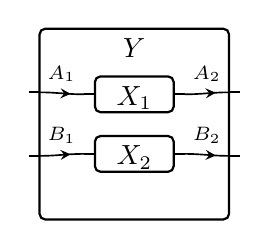
\begin{tikzpicture}[oriented WD, bbx=1em, bby=1ex]
 \node[bb={1}{1},bb name=$X_1$] (X1) {};
 \node[bb={1}{1},below =2 of X1, bb name=$X_2$] (X2) {};
 \node[bb={2}{2}, fit={($(X1.north west)+(-1,3)$) ($(X2.south)+(0,-3)$) ($(X2.east)+(1,0)$)}, bb name = $Y$] (Y) {};
%
 \draw[ar] (Y_in1') to (X1_in1);
 \draw[ar] (Y_in2') to (X2_in1);
 \draw[ar] (X1_out1) to (Y_out1');
 \draw[ar] (X2_out1) to (Y_out2');
 \draw[label] 
	node at ($(Y_in1')!.5!(X1_in1)+(0,7pt)$)  {$A_1$}
	node at ($(Y_in2')!.5!(X2_in1)+(0,7pt)$)   {$B_1$}
	node at ($(X1_out1)!.5!(Y_out1')+(0,7pt)$)  {$A_2$}
	node at ($(X2_out1)!.5!(Y_out2')+(0,7pt)$) {$B_2$};
\end{tikzpicture}
\end{equation}

\begin{equation}\label{junky}\tag{junky}
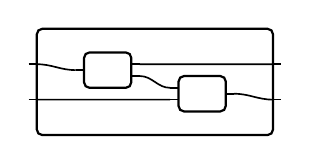
\begin{tikzpicture}[oriented WD, bb min width =.6cm, bb port sep =.5, bby=.3cm, bbx=.6cm,bb port length=3pt]
  \node[bb={1}{2}] (X1) {};
  \node[bb={2}{1}, below right=-.5 and 1 of X1] (X2) {};
  \node[bb={2}{2}, fit=(X1) (X2)] (Y) {};
  \draw (Y_in1') to (X1_in1);
  \draw (Y_in2') to (X2_in2);
  \draw (X1_out1) to (Y_out1');
  \draw (X1_out2) to (X2_in1);
  \draw (X2_out1) to (Y_out2');
\end{tikzpicture}
\end{equation}

\begin{equation}\label{blue_sub}\tag{blue substitution}
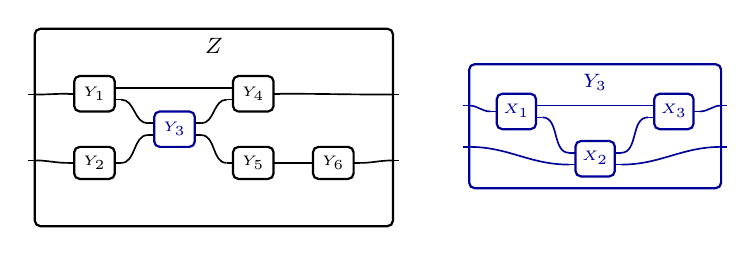
\begin{tikzpicture}[oriented WD,bb min width =.5cm, bbx=.5cm, bb port sep =1,bb port length=.08cm, bby=.15cm]
\begin{scope}[blue!60!black]
	\node[bb={1}{2},bb name = {\tiny$X_{1}$}] (X11) {};
	\node[bb={2}{2},below right=of X11,bb name = {\tiny$X_{2}$}] (X12) {};
	\node[bb={2}{1}, above right=of X12,bb name = {\tiny$X_{3}$}] (X13) {};
	\node[bb={2}{2}, fit={($(X11.north west)+(.3,1.5)$) (X12)  ($(X13.east)+(-.3,0)$)},bb name = {\scriptsize $Y_3$}] (Y1) {};
	\draw (Y1_in1') to (X11_in1);	
	\draw (Y1_in2') to (X12_in2);
	\draw (X11_out1) to (X13_in1);
	\draw (X11_out2) to (X12_in1);
	\draw (X12_out1) to (X13_in2);
	\draw (X12_out2) to (Y1_out2');
	\draw (X13_out1) to (Y1_out1');
\end{scope}

\node [bb={1}{2}, below left =1 and 9 of $(Y1.north west)$] (Y1) {\tiny $Y_1$};
\node [bb={1}{1},below=3 of Y1] (Y2) {\tiny $Y_2$};
\node [bb={2}{2}, blue!60!black,below right = 0 and 1 of Y1] (Y3) {\tiny $Y_3$};
\node [bb={2}{1},right=3 of Y1] (Y4) {\tiny $Y_4$};
\node [bb={1}{1},right=3 of Y2] (Y5) {\tiny $Y_5$};
\node [bb={1}{1},right=1of Y5] (Y6) {\tiny $Y_6$};

\node [bb={2}{2},fit={($(Y1.north)+(0,3)$) ($(Y2.south west)+(0,-3)$) (Y3) (Y4) (Y5) (Y6)}, bb name={\footnotesize $Z$}] (Z) {};
\draw (Z_in1') to (Y1_in1);
\draw (Z_in2') to (Y2_in1);
\draw (Y1_out1) to (Y4_in1);
\draw (Y1_out2) to (Y3_in1);
\draw (Y2_out1) to (Y3_in2);
\draw (Y3_out1) to (Y4_in2); 
\draw (Y3_out2) to (Y5_in1);
\draw (Y4_out1) to (Z_out1');
\draw (Y5_out1) to (Y6_in1);
\draw (Y6_out1) to (Z_out2');
\end{tikzpicture}
\end{equation}

\begin{equation}\label{substitution2}\tag{substitution2}
\begin{tikzpicture}[oriented WD,bb min width =.5cm, bbx=.5cm, bb port sep =1,bb port length=.08cm, bby=.15cm]
  \begin{scope}[blue!60!black]
  	\node[bb={1}{2},bb name = {\tiny$f_{1}$}] (X11) {};
  	\node[bb={2}{2},below right=of X11,bb name = {\tiny$f_{2}$}] (X12) {};
  	\node[bb={2}{1}, above right=of X12,bb name = {\tiny$f_{3}$}] (X13) {};
  	\node[bb={0}{0}, fit={($(X11.north west)+(.3,1.5)$) (X12)  ($(X13.east)+(-.3,0)$)},bb name = {\scriptsize $g_3$}] (Sub) {};
  	\node[coordinate] at (Sub.west|-X11_in1) (Sub_in1) {};
  	\node[coordinate] at (Sub.west|-X12_in2) (Sub_in2) {};
  	\node[coordinate] at (Sub.east|-X12_out2) (Sub_out2) {};
  	\node[coordinate] at (Sub.east|-X13_out1) (Sub_out1) {};
  	\draw[shorten <= -2pt] (Sub_in1) to (X11_in1);	
  	\draw[shorten <= -2pt] (Sub_in2) to (X12_in2);
  	\draw (X11_out1) to (X13_in1);
  	\draw (X11_out2) to (X12_in1);
  	\draw (X12_out1) to (X13_in2);
  	\draw[shorten >= -2pt] (X12_out2) to (Sub_out2);
  	\draw[shorten >= -2pt] (X13_out1) to (Sub_out1);
  \end{scope}
%  
  \node [bb={1}{2}, below right =2 and 9 of $(Sub.north west)$] (Y1) {\tiny $g_1$};
  \node [bb={1}{1},below=3 of Y1] (Y2) {\tiny $g_2$};
  \node [bb={2}{2}, blue!60!black,below right = 0 and 1 of Y1] (Y3) {\tiny $g_3$};
  \node [bb={2}{1},right=3 of Y1] (Y4) {\tiny $g_4$};
  \node [bb={1}{1},right=3 of Y2] (Y5) {\tiny $g_5$};
  \node [bb={0}{0},fit={($(Y1.north)+(0,2)$) (Y2.south west) (Y3) (Y4) (Y5)}, bb name={\footnotesize $h$}] (Z) {};
  \node[coordinate] at (Z.west|-Y1_in1) (Z_in1) {};
  \node[coordinate] at (Z.west|-Y2_in1) (Z_in2) {};
  \node[coordinate] at (Z.east|-Y4_out1) (Z_out1) {};
  \node[coordinate] at (Z.east|-Y5_out1) (Z_out2) {};
  \draw (Z_in1) to (Y1_in1);
  \draw (Z_in2) to (Y2_in1);
  \draw (Y4_out1) to (Z_out1);
  \draw (Y5_out1) to (Z_out2);
  \draw (Y1_out1) to (Y4_in1);
  \draw (Y1_out2) to (Y3_in1);
  \draw (Y2_out1) to (Y3_in2);
  \draw (Y3_out1) to (Y4_in2); 
  \draw (Y3_out2) to (Y5_in1);
%
	\draw[blue, dotted] (Sub.north east) -- (Y3.north west);
	\draw[blue, dotted] (Sub.south east) -- (Y3.south west);
%
  \node [bb={1}{2}, right = 9 of $(Y1)$] (YY1) {\tiny $g_1$};
  \node [bb={1}{1},below=3 of YY1] (YY2) {\tiny $g_2$};
	\node [bb={1}{2}, below right=-1 and 1 of YY1, bb name = {\tiny$f_{1}$}] (XX11) {};
  \node [bb={2}{2}, below right=-1 and 1 of XX11,bb name = {\tiny$f_{2}$}] (XX12) {};
  \node [bb={2}{1}, above right=-1 and 1 of XX12,bb name = {\tiny$f_{3}$}] (XX13) {};
  \node [bb={2}{1}, above right=-1 and 1 of XX13] (YY4) {\tiny $g_4$};
  \node [bb={1}{1}, below=3 of YY4] (YY5) {\tiny $g_5$};
  \node [bb={0}{0},fit={($(YY1.north)+(0,2)$) (YY2.south west) (YY4) (YY5)}, bb name={\footnotesize $h$}] (ZZ) {};
  \node[coordinate] at (ZZ.west|-YY1_in1) (ZZ_in1) {};
  \node[coordinate] at (ZZ.west|-YY2_in1) (ZZ_in2) {};
  \node[coordinate] at (ZZ.east|-YY4_out1) (ZZ_out1) {};
  \node[coordinate] at (ZZ.east|-YY5_out1) (ZZ_out2) {};
  \draw (ZZ_in1) to (YY1_in1);
  \draw (ZZ_in2) to (YY2_in1);
  \draw (YY4_out1) to (ZZ_out1);
  \draw (YY5_out1) to (ZZ_out2);
  \draw (YY1_out1) to (YY4_in1);
  \draw (YY1_out2) to (XX11_in1);
  \draw (YY2_out1) to (XX12_in2);
  \draw (XX13_out1) to (YY4_in2); 
  \draw (XX12_out2) to (YY5_in1);
  \draw (XX11_out1) to (XX13_in1);
  \draw (XX11_out2) to (XX12_in1);
  \draw (XX12_out1) to (XX13_in2);
%
	\node at ($(Z.east)!.5!(ZZ.west)$) {$\leadsto$};
\end{tikzpicture}
\end{equation}

\begin{equation}\label{terminate}\tag{terminate}
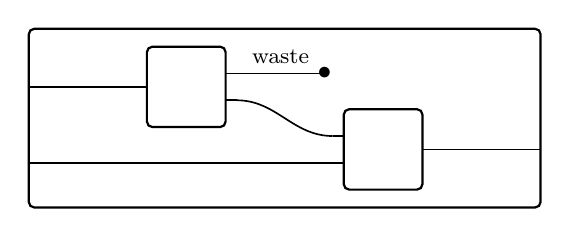
\begin{tikzpicture}[oriented WD]
	\node[bb={1}{2}] (A) {};
	\node[bb={2}{1}, below right=-1 and 1 of A] (B) {};
	\node[bb={0}{0}, fit=(A) (B)] (outer) {};
	\node[right=.6 of A_out1] (kill) {$\bullet$};
	\draw (outer.west|-A_in1) -- (A_in1);
	\draw (outer.west|-B_in2) -- (B_in2);
	\draw (A_out1) to node[above, font=\footnotesize] {waste} (kill.center);
	\draw (A_out2) to (B_in1);
	\draw (B_out1) -- (B_out1-|outer.east);
\end{tikzpicture}
\end{equation}

\begin{equation}\label{IAN:feedforward}\tag{IAN: feedforward}
\begin{tabular}{c|c|c}
\small {Interfaces}&\small {Arrangements}&\small {Nesting}\\\hline
~&&\\
\parbox{.5in}{
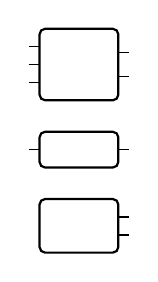
\begin{tikzpicture}[oriented WD, bby=1ex]
  \node[bb={3}{2}] (X1) {};
  \node[bb={1}{1}, below=.4cm of X1] (X2) {};
  \node[bb={0}{2}, below=.4cm of X2] (X3) {};   
\end{tikzpicture}
}
&
\;\;\parbox{1.3in}{
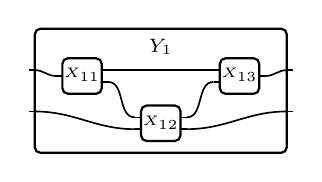
\begin{tikzpicture}[oriented WD,bb min width =.5cm, bbx=.5cm, bb port sep =1,bb port length=.08cm, bby=.15cm]
\path (0,0) pic {Yonepart};
\end{tikzpicture}
}
&
\;\;\parbox{2in}{
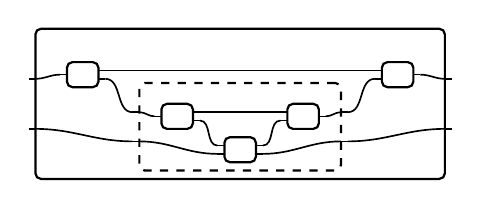
\begin{tikzpicture}[oriented WD, bb small]
  \node[bb={1}{2}] (X1) {};
  \node[bb={2}{1},right=9 of X1] (X2) {};
  
  \node[bb={1}{2},below right = 2 and 2 of X1] (X11) {};
  \node[bb={2}{2},below right=of X11] (X12) {};
  \node[bb={2}{1}, above right=of X12] (X13) {};
  \node[bb={2}{2}, dashed, fit={($(X11.north west)+(.3,1.5)$) (X12)  ($(X13.east)+(-.3,0)$)}] (Y1) {};
  
  \node[bb={2}{2}, fit={($(X1.north west)+(0,3)$) (Y1) (X2)}] (Z) {};
  \draw (Y1_in1') to (X11_in1);	
  \draw (Y1_in2') to (X12_in2);
  \draw (X11_out1) to (X13_in1);
  \draw (X11_out2) to (X12_in1);
  \draw (X12_out1) to (X13_in2);
  \draw (X12_out2) to (Y1_out2');
  \draw (X13_out1) to (Y1_out1');
  \draw (Z_in1') to (X1_in1);
  \draw (Z_in2') to (Y1_in2);
  \draw (X1_out1) to (X2_in1);
  \draw (X1_out2) to (Y1_in1);
  \draw (Y1_out1) to (X2_in2);
  \draw (Y1_out2) to (Z_out2');
  \draw (X2_out1) to (Z_out1');
\end{tikzpicture}
}\\
&&\parbox{1.7in}{(Getting a sense of how\\ fractals are a special case?)}
\end{tabular}
\end{equation}

\begin{equation}
\begin{tikzpicture}
\node (p1) {
	\begin{tikzpicture}[oriented WD, bb small, font=\tiny]
	\node[bb={1}{1}] (X1) {\tiny$t_1$};
  	\node[bb={1}{1}, right=.5 of X1] (X2) {\tiny$t_2$};
	\node[bb={1}{1}, right=2 of X2] (X3) {\tiny$t_3$};
	\node[bb={0}{0}, thin, gray, fit=(X1)(X2)] (X12) {};
	\node[bb={1}{1}, fit=(X12) (X3)] (Y) {};
	\draw (Y_in1') to (X1_in1);
	\draw (X1_out1) to (X2_in1);
	\draw (X2_out1) to (X3_in1);
	\draw (X3_out1) to (Y_out1');
	\node[bb={1}{1}] (X1) {\tiny$t_1$};
	\end{tikzpicture}
};
\node (p2) [right=1 of p1] {
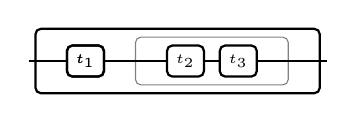
\begin{tikzpicture}[oriented WD, bb small, font=\tiny]
	\node[bb={1}{1}] (X1') {\tiny$t_1$};
  	\node[bb={1}{1}, right=2 of X1'] (X2') {\tiny$t_2$};
	\node[bb={1}{1}, right=.5 of X2'] (X3') {\tiny$t_3$};
	\node[bb={0}{0}, thin, gray, fit=(X2')(X3')] (X23') {};
	\node[bb={1}{1}, fit=(X1') (X23')] (Y') {};
	\draw (Y'_in1') to (X1'_in1);
	\draw (X1'_out1) to (X2'_in1);
	\draw (X2'_out1) to (X3'_in1);
	\draw (X3'_out1) to (Y'_out1');
	\node[bb={1}{1}] (X1') {\tiny$t_1$};
\end{tikzpicture}
};
\node at ($(p1.east)!.5!(p2.west)$) {$=$};
\end{tikzpicture}
\end{equation}

\begin{equation}
\begin{tikzpicture}[oriented WD, bb small, font=\tiny]
\node (p1) {
\begin{tikzpicture}[oriented WD, bb small, font=\tiny]
  \node[bb={1}{1}, gray, thin] (x1) {\vphantom{$t$}};
  \node[bb={1}{1}, right=of x1] (x2) {$t$};
  \node[bb={1}{1}, inner xsep=10pt, inner ysep=10pt, fit=(x1) (x2)] (outer) {};
  \node[above] at (outer.south) {};
  \draw (x1_in1') -- (x1_out1');
  \draw (outer_in1') -- node[above] {$A$} (x1_in1);
  \draw (x1_out1) -- node[above] {$A$} (x2_in1);
  \draw (x2_out1) -- node[above] {$B$} (outer_out1');
\end{tikzpicture}
};
\node (p2) [right=of p1]
{
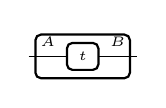
\begin{tikzpicture}[oriented WD, bb small, font=\tiny]
  \node[bb={1}{1}] (x2) {$t$};
  \node[bb={1}{1}, inner xsep=10pt, inner ysep=10pt, fit=(x2)] (outer) {};
  \draw (outer_in1') -- node[above] {$A$} (x2_in1);
  \draw (x2_out1) -- node[above] {$B$} (outer_out1');
\end{tikzpicture}
};
\node (p3) [right=of p2]
{
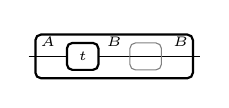
\begin{tikzpicture}[oriented WD, bb small, font=\tiny]
  \node[bb={1}{1}, gray, thin] (x1) {\vphantom{$t$}};
  \node[bb={1}{1}, left=of x1] (x2) {$t$};
  \node[bb={1}{1}, inner xsep=10pt, inner ysep=10pt, fit=(x1) (x2)] (outer) {};
  \node[above] at (outer.south) {};
  \draw (x1_in1') -- (x1_out1');
  \draw (outer_in1') -- node[above] {$A$} (x2_in1);
  \draw (x2_out1) -- node[above] {$B$} (x1_in1);
  \draw (x1_out1) -- node[above] {$B$} (outer_out1');
\end{tikzpicture}
};
\node[font=\normalsize] at ($(p1.east)!.5!(p2.west)$) {=};
\node[font=\normalsize] at ($(p2.east)!.5!(p3.west)$) {=};
\end{tikzpicture}
\end{equation}

\begin{equation}
\begin{tikzpicture}
\node (p1) {
\begin{tikzpicture}[oriented WD, bb small, font=\tiny]
    \node[bb={1}{1}] (t1) {$t_1$};
    \node[bb={1}{1}, below=of t1] (t2) {$t_2$};
    \node[bb={1}{1}, below=2 of t2] (t3) {$t_3$};
    \node[bb={0}{0}, thin, gray, fit = (t1) (t2)] (t12) {};
    \node[bb={0}{0}, fit= (t12) (t3)] (outer) {};
    \begin{scope}[shorten >=-1.5pt]
        \draw (t1_in1) -- (outer.west|-t1_in1);
        \draw (t1_out1) -- (outer.east|-t1_out1);
        \draw (t2_in1) -- (outer.west|-t2_in1);
        \draw (t2_out1) -- (outer.east|-t2_out1);
        \draw (t3_in1) -- (outer.west|-t3_in1);
        \draw (t3_out1) -- (outer.east|-t3_out1);
    \end{scope}
\end{tikzpicture}
};
%
\node (p2) [right=1 of p1] {
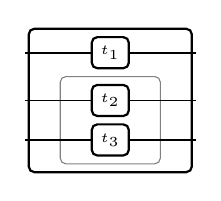
\begin{tikzpicture}[oriented WD, bb small, font=\tiny]
    \node[bb={1}{1}] (t1') {$t_1$};
    \node[bb={1}{1}, below=2 of t1'] (t2') {$t_2$};
    \node[bb={1}{1}, below=of t2'] (t3') {$t_3$};
    \node[bb={0}{0}, thin, gray, fit=(t2') (t3')] (t23') {};
    \node[bb={0}{0}, fit= (t1') (t23')] (outer') {};
    \begin{scope}[shorten >=-1.5pt]
        \draw (t1'_in1) -- (outer'.west|-t1'_in1);
        \draw (t1'_out1) -- (outer'.east|-t1'_out1);
        \draw (t2'_in1) -- (outer'.west|-t2'_in1);
        \draw (t2'_out1) -- (outer'.east|-t2'_out1);
        \draw (t3'_in1) -- (outer'.west|-t3'_in1);
        \draw (t3'_out1) -- (outer'.east|-t3'_out1);
    \end{scope}
\end{tikzpicture}
};
\node[font=\normalsize] at ($(p1.east)!.5!(p2.west)$) {=};
\end{tikzpicture}
\end{equation}

\begin{equation}
\begin{tikzpicture}
\node (p1) {
\begin{tikzpicture}[oriented WD, bb small, font=\tiny]
    \node[bb={1}{1}] (t11) {$t_{11}$};
    \node[bb={1}{1}, right=.5 of t11] (t12) {$t_{12}$};
    \node[bb={1}{1}, below=3 of t11] (t21) {$t_{21}$};
    \node[bb={1}{1}, right=.5 of t21] (t22) {$t_{22}$};
    \node[bb={0}{0}, thin, gray, fit=(t11) (t12)] (t1) {};
    \node[bb={0}{0}, thin, gray, fit=(t21) (t22)] (t2) {};
    \node[bb={0}{0}, fit=(t1) (t2)] (outer) {};
    \draw (t11_out1) -- (t12_in1);
    \draw (t21_out1) -- (t22_in1);
    \begin{scope}[shorten >=-1.5pt]
        \draw (t11_in1) -- (t11_in1-|outer.west);
        \draw (t21_in1) -- (t21_in1-|outer.west);
        \draw (t12_out1) -- (t12_out1-|outer.east);
        \draw (t22_out1) -- (t22_out1-|outer.east);
    \end{scope}
\end{tikzpicture}
};
%
\node (p2) [right=1 of p1] {
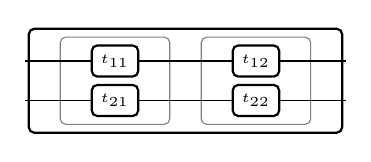
\begin{tikzpicture}[oriented WD, bb small, font=\tiny]
    \node[bb={1}{1}] (t11) {$t_{11}$};
    \node[bb={1}{1}, right=3 of t11] (t12) {$t_{12}$};
    \node[bb={1}{1}, below=of t11] (t21) {$t_{21}$};
    \node[bb={1}{1}, right=3 of t21] (t22) {$t_{22}$};
    \node[bb={0}{0}, thin, gray, fit=(t11) (t21)] (t1) {};
    \node[bb={0}{0}, thin, gray, fit=(t12) (t22)] (t2) {};
    \node[bb={0}{0}, fit=(t1) (t2)] (outer) {};
    \draw (t11_out1) -- (t12_in1);
    \draw (t21_out1) -- (t22_in1);
    \begin{scope}[shorten >=-1.5pt]
        \draw (t11_in1) -- (t11_in1-|outer.west);
        \draw (t21_in1) -- (t21_in1-|outer.west);
        \draw (t12_out1) -- (t12_out1-|outer.east);
        \draw (t22_out1) -- (t22_out1-|outer.east);
    \end{scope}
\end{tikzpicture}
};
\node[font=\normalsize] at ($(p1.east)!.5!(p2.west)$) {=};
\end{tikzpicture}
\end{equation}

\subsection{Splitting}

\begin{equation}\label{updrdt}\tag{upd and rdt}
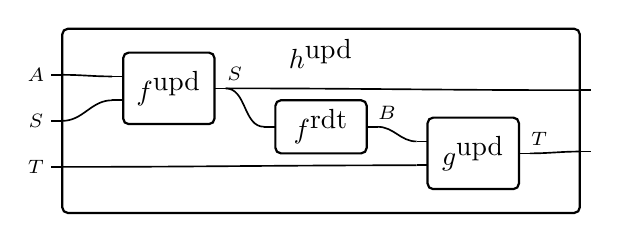
\begin{tikzpicture}[oriented WD, bbx=1.1em, bb min width=3.3em, bby=2ex, bb port sep = 1]
	\node[bb={2}{1}] (X1) {$\upd{f}$};
	\node[bb={1}{1}, below right=-1 and 2 of X1] (X2) {$\rdt{f}$};
	\node[bb={2}{1}, below right=-1.5 and 2 of X2] (X3) {$\upd{g}$};
	\node[bb={3}{2}, fit={($(X1.north west)+(-1,0)$) (X2) ($(X3.south east)+(1,0)$)}, bb name = {$\upd{h}$}] (Y) {};
	%
	\draw (Y_in1') to (X1_in1) ;
	\draw (Y_in2') to (X1_in2);
	\draw (X1_out1) to (Y_out1');
	\draw (X1_out1) to (X2_in1);
	\draw (X2_out1) to (X3_in1);
	\draw (Y_in3') to (X3_in2);
	\draw (X3_out1) to (Y_out2');
	\draw[label]
		node at ($(Y_in1)+(-.5,0)$) {$A$}
		node at ($(Y_in2)+(-.5,0)$) {$S$}
		node at ($(Y_in3)+(-.5,0)$) {$T$}
		node at ($(X1_out1)+(.3,.6)$) {$S$}
		node at ($(X2_out1)+(.3,.6)$) {$B$}
		node at ($(X3_out1)+(.3,.6)$) {$T$};
\end{tikzpicture}
\qquad\qquad
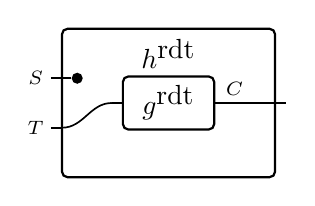
\begin{tikzpicture}[oriented WD, bbx=1.1em, bb min width=3.3em, bby=2ex, bb port sep = 1]
	\node[bb={1}{1}] (X) {$\rdt{g}$};
	\node[bb={2}{1}, fit={($(X.north west)+(-1,1)$) ($(X.south east)+(1,-1)$)}, bb name={$\rdt{h}$}] (Y) {};
	\node [circle,minimum size=4pt, inner sep=0, fill] (dot) at ($(Y_in1')+(.5,0)$) {};
	%
	\draw (Y_in1') to (dot);
	\draw (Y_in2') to (X_in1);
	\draw (X_out1) to (Y_out1');
	\draw[label]
		node at ($(Y_in1)-(.5,0)$) {$S$}
		node at ($(Y_in2)-(.5,0)$) {$T$}
		node at ($(X_out1)+(.3,.6)$) {$C$};
\end{tikzpicture}
\end{equation}

\begin{equation}\label{split_leftright}\tag{split left/right}
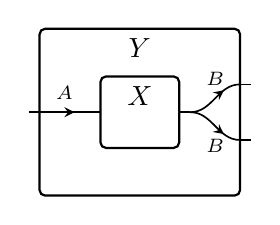
\begin{tikzpicture}[oriented WD, bbx=1em, bby=1ex, bb port sep=3 pt]
 	\node[bb={1}{1},bb name=$X$] (X) {};
	\node[bb={1}{2}, fit={(X) ($(X.north east)+(1.2,3)$) ($(X.south west)+(-1.2,-3)$)}, bb name = $Y$] (Y) {};
%
	\draw[ar] (Y_in1') to (X_in1);
	\draw[ar] (X_out1) to (Y_out1');
	\draw[ar] (X_out1) to (Y_out2');
	\draw[label] 
		node at ($(Y_in1')!.5!(X_in1)+(0,7pt)$)  {$A$}
		node at ($(X_out1)!.5!(Y_out1')+(0,7pt)$)   {$B$}
		node at ($(X_out1)!.5!(Y_out2')-(0,7pt)$)   {$B$};
\end{tikzpicture}
\qquad\qquad
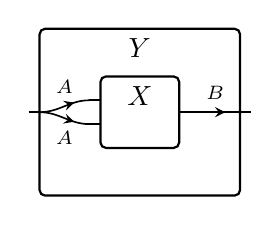
\begin{tikzpicture}[oriented WD, bbx=1em, bby=1ex, bb port sep=2 pt]
 	\node[bb={2}{1},bb name=$X$] (X) {};
	\node[bb={1}{1}, fit={(X) ($(X.north east)+(1.2,3)$) ($(X.south west)+(-1.2,-3)$)}, bb name = $Y$] (Y) {};
%
	\draw[ar] (Y_in1') to (X_in1);
	\draw[ar] (Y_in1') to (X_in2);
	\draw[ar] (X_out1) to (Y_out1');
	\draw[label] 
		node at ($(Y_in1')!.5!(X_in1)+(0,7pt)$)  {$A$}
		node at ($(Y_in1')!.5!(X_in2)-(0,7pt)$)   {$A$}
		node at ($(X_out1)!.5!(Y_out1')+(0,7pt)$)   {$B$};
\end{tikzpicture}
\end{equation}

\begin{equation}\label{split_and_terminate}\tag{split and terminate}
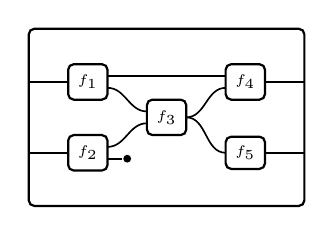
\begin{tikzpicture}[oriented WD,bb min width =.5cm, bbx=.5cm, bb port sep =1,bb port length=0, bby=.15cm]
\node [bb={1}{2}] (Y1) {\tiny $f_1$};
\node [bb={1}{2},below=3 of Y1] (Y2) {\tiny $f_2$};
\node [bb={2}{1},below right = 0 and 1 of Y1] (Y3) {\tiny $f_3$};
\node [bb={2}{1},right=3 of Y1] (Y4) {\tiny $f_4$};
\node [bb={1}{1},right=3 of Y2] (Y5) {\tiny $f_5$};
\node [bb={2}{2},fit={($(Y1.north)+(0,2)$) ($(Y2.south west)+(0,-2)$) (Y4) (Y5)}] (Z) {};
\node [circle, fill, inner sep=1pt] at ($(Y2_out2)+(0.5,0)$) (kill) {};
\draw (Z_in1'|-Y1_in1) to (Y1_in1);
\draw (Z_in2'|-Y2_in1) to (Y2_in1);
\draw (Y1_out1) to (Y4_in1);
\draw (Y1_out2) to (Y3_in1);
\draw (Y2_out1) to (Y3_in2);
\draw (Y2_out2) to (kill);
\draw (Y3_out1) to (Y4_in2); 
\draw (Y3_out1) to (Y5_in1);
\draw (Y4_out1) to (Z_out1'|-Y4_out1);
\draw (Y5_out1) to (Z_out2'|-Y5_out1);
\end{tikzpicture}
\end{equation}


\begin{equation}\label{meringue}\tag{meringue}
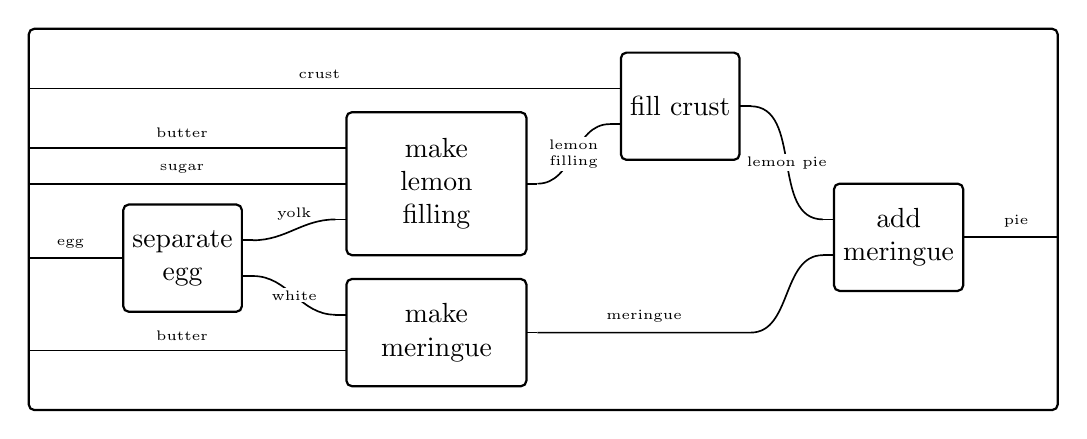
\begin{tikzpicture}[oriented WD, align=center, bbx=1.2cm, bby=2ex]
	\node[bb={3}{1}, bb min width=.9in] (filling) {make\\lemon\\filling};
	\node[bb={2}{1}, bb min width=.9in, below=of filling] (meringue) {make\\meringue};
	\node at ($(filling.west)!.5!(meringue.west)$) (helper) {};
	\node[bb={1}{2}, left = of helper] (separate) {separate\\egg};
	\node[bb={2}{1}, above right = -2 and 1 of filling] (fill) {fill crust};
	\node[bb={2}{1}, below right = of fill] (finish) {add\\meringue};
	\node[bb={0}{0}, fit=(separate) (meringue) (fill) (finish)] (pie) {};
%
\begin{scope}[font=\tiny]
	\draw (pie.west|-fill_in1) to node[above] {crust} (fill_in1);
	\draw (pie.west|-filling_in1) to node[above] {butter} (filling_in1);
	\draw (pie.west|-filling_in2) to node[above] {sugar} (filling_in2);
	\draw (pie.west|-separate_in1) to node[above] {egg} (separate_in1);
	\draw (pie.west|-meringue_in2) to node[above] {butter} (meringue_in2);
	\draw (separate_out1) to node[above] {yolk} (filling_in3);
	\draw (separate_out2) to node[fill=white, inner sep=0.8pt] {white} (meringue_in1);
	\draw (filling_out1) to node[fill=white, inner sep=0.8pt] {lemon\\filling} (fill_in2);
	\draw (fill_out1) to node[fill=white, inner sep=0.8pt] {lemon pie} (finish_in1);
	\draw let \p1=(fill.east|-meringue_out1), \n1=\bbportlen in
		(meringue_out1) to node[above] {meringue} (\x1+\n1,\y1) to (finish_in2);
	\draw (finish_out1) to node[above] {pie} (finish_out1-|pie.east);
\end{scope}
\end{tikzpicture}
\end{equation}


\begin{figure}
\[
C
\left(\quad
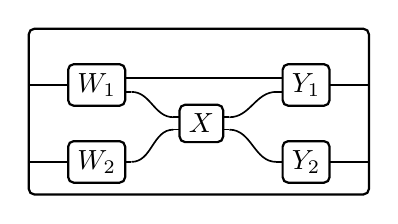
\begin{tikzpicture}[oriented WD,bb min width =.5cm, bbx=.5cm, bb port sep =1,bb port length=.08cm, bby=.15cm, baseline=(Z)]
  \node [bb={1}{2}] (Y1) { $W_1$};
  \node [bb={1}{1}, below=3 of Y1] (Y2) { $W_2$};
  \coordinate (W) at ($(Y1)!.5!(Y2)$);
  \node [bb={2}{1},right=4 of Y1] (Y4) { $Y_1$};
  \node [bb={1}{1},right=4 of Y2] (Y5) { $Y_2$};
  \coordinate (Y) at ($(Y4)!.5!(Y5)$);
  \node [bb={2}{2}] at ($(W)!.5!(Y)$) (Y3) { $X$};  
  \node [bb={0}{0},fit={($(Y1.north)+(0,2)$) (Y2.south west) (Y3) (Y4) (Y5)}] (Z) {};
  \node[coordinate] at (Z.west|-Y1_in1) (Z_in1) {};
  \node[coordinate] at (Z.west|-Y2_in1) (Z_in2) {};
  \node[coordinate] at (Z.east|-Y4_out1) (Z_out1) {};
  \node[coordinate] at (Z.east|-Y5_out1) (Z_out2) {};
  \draw (Z_in1) to (Y1_in1);
  \draw (Z_in2) to (Y2_in1);
  \draw (Y4_out1) to (Z_out1);
  \draw (Y5_out1) to (Z_out2);
  \draw (Y1_out1) to (Y4_in1);
  \draw (Y1_out2) to (Y3_in1);
  \draw (Y2_out1) to (Y3_in2);
  \draw (Y3_out1) to (Y4_in2); 
  \draw (Y3_out2) to (Y5_in1);
\end{tikzpicture}
\quad\right)
\qquad
\leq
\qquad
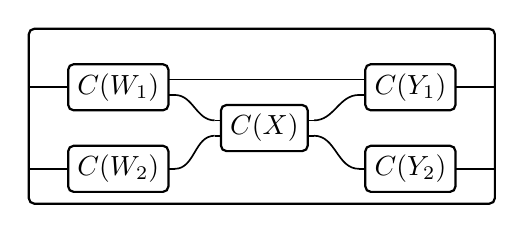
\begin{tikzpicture}[oriented WD,bb min width =.5cm, bbx=.5cm, bb port sep =1,bb port length=.08cm, bby=.15cm, baseline=(Z)]
  \node [bb={1}{2}] (Y1) { $C(W_1)$};
  \node [bb={1}{1}, below=3 of Y1] (Y2) { $C(W_2)$};
  \coordinate (W) at ($(Y1)!.5!(Y2)$);
  \node [bb={2}{1},right=5 of Y1] (Y4) { $C(Y_1)$};
  \node [bb={1}{1},right=5 of Y2] (Y5) { $C(Y_2)$};
  \coordinate (Y) at ($(Y4)!.5!(Y5)$);
  \node [bb={2}{2}] at ($(W)!.5!(Y)$) (Y3) { $C(X)$};  
  \node [bb={0}{0},fit={($(Y1.north)+(0,2)$) (Y2.south west) (Y3) (Y4) (Y5)}] (Z) {};
  \node[coordinate] at (Z.west|-Y1_in1) (Z_in1) {};
  \node[coordinate] at (Z.west|-Y2_in1) (Z_in2) {};
  \node[coordinate] at (Z.east|-Y4_out1) (Z_out1) {};
  \node[coordinate] at (Z.east|-Y5_out1) (Z_out2) {};
  \draw (Z_in1) to (Y1_in1);
  \draw (Z_in2) to (Y2_in1);
  \draw (Y4_out1) to (Z_out1);
  \draw (Y5_out1) to (Z_out2);
  \draw (Y1_out1) to (Y4_in1);
  \draw (Y1_out2) to (Y3_in1);
  \draw (Y2_out1) to (Y3_in2);
  \draw (Y3_out1) to (Y4_in2); 
  \draw (Y3_out2) to (Y5_in1);
\end{tikzpicture}
\]
\caption{Channel capacity is a strict monoidal lax functor $\mathsf{Stoch}\to\mathcal{R}$, where $(\mathsf{Stoch},\otimes)$ is the monoidal category of stochastic matrices, and $\mathcal{R}=([0,\infty],(\infty,\min),\geq,(+,0))$ is the lax monoidal po-monoid with one object, denoted $\cdot$, with $\mathrm{Hom}(\cdot,\cdot):=[0,\infty]$, with identity $\mathrm{id}_\cdot:=\infty$ and composition given by $\min$, with local partial order (po) structure given by the usual $\geq$, and with lax monoidal structure (the interchange law is a lax functor) that is given by  $+$ and $0$.
The above diagram says the following symbolically:
}
\vspace{-.2in}
\[
  C\big(
  (W_1\otimes W_2)\fatsemi (\mathrm{id}\otimes X)\fatsemi (Y_1\otimes Y_2)
  \big)
  \leq
  \min\Big(\big(C(W_1)+C(W_2)\big), C(X), \big(C(Y_1)+C(Y_2)\big)\Big).
\]

The theorem also holds when replacing the $\otimes$ monoidal structure on $\mathsf{Stoch}$ with the $\oplus$ monoidal structure and replacing channel capacity $C$ with its exponent, $\exp C$. That is,
\begin{multline*}
  \exp C\big(
  (W_1\oplus W_2)\fatsemi (\mathrm{id}\oplus X)\fatsemi (Y_1\oplus Y_2)
  \big)\\
  \leq
  \min\Big(\big(\exp C(W_1)+\exp C(W_2)\big), \exp C(X), \big(\exp C(Y_1)+\exp C(Y_2)\big)\Big).
\end{multline*}
 
\end{figure}

\begin{equation}\label{nnet}\tag{nnet}
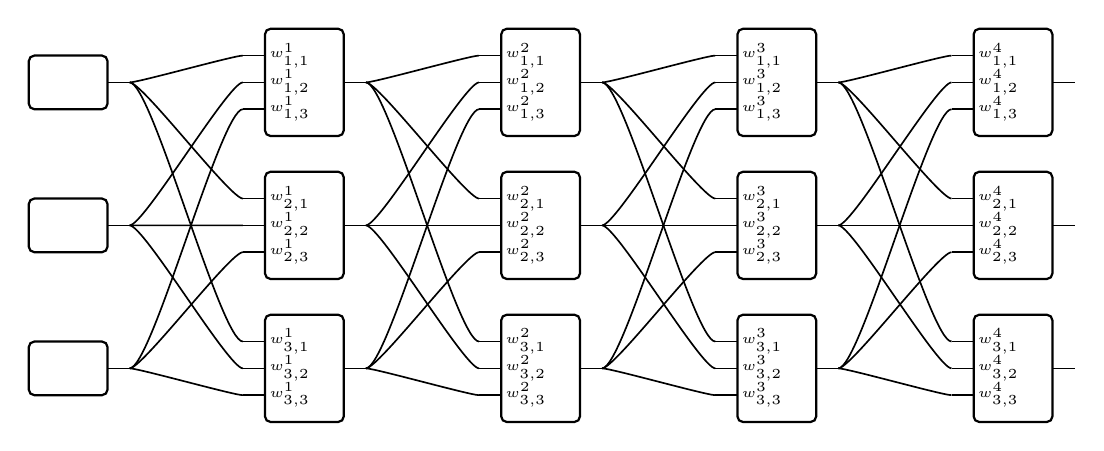
\begin{tikzpicture}[oriented WD, bb port sep=1.5, scale=2]
	\tikzmath{
	int \hidden, \depth, \hiddeninc, \incsqrd;
	\hidden=3; %Set this
	\depth=3;  %Set this
	\hiddeninc=\hidden+1;
	\incsqrd = \hiddeninc*\hiddeninc;
	}
	\foreach \j in {1,...,\depth} {
			\node[bb={0}{1}] (N0\j) at (0,\incsqrd-\hiddeninc*\j) {};
		}
	\foreach \i [remember=\i as \lasti (initially 0)] in {1,...,\hidden} {
		\foreach \j in {1,...,\depth} {
			\node[bb={\depth}{1}] (N\i\j) at (\i,\incsqrd-\hiddeninc*\j) {};
			\foreach \jj in {1,...,\depth} {
				\draw (N\lasti\jj_out1) to[looseness=0.2] (N\i\j_in\jj);
				\node [right=6pt, font=\tiny] at (N\i\j_in\jj) {$w^\i_{\j,\jj}$};
			}
		}
	}
	\foreach \j in {1,...,\depth} {
			\node[bb={\depth}{1}] (N\hiddeninc\j) at (\hiddeninc,\incsqrd-\hiddeninc*\j) {};
			\foreach \jj in {1,...,\depth} {
				\draw (N\hidden\jj_out1) to[looseness=0.2] (N\hiddeninc\j_in\jj);
				\node [right=6pt, font=\tiny] at (N\hiddeninc\j_in\jj) {$w^\hiddeninc_{\j,\jj}$};
			}
		}
\end{tikzpicture}
\end{equation}

\begin{equation}\label{nnet pretty}\tag{nnet pretty}
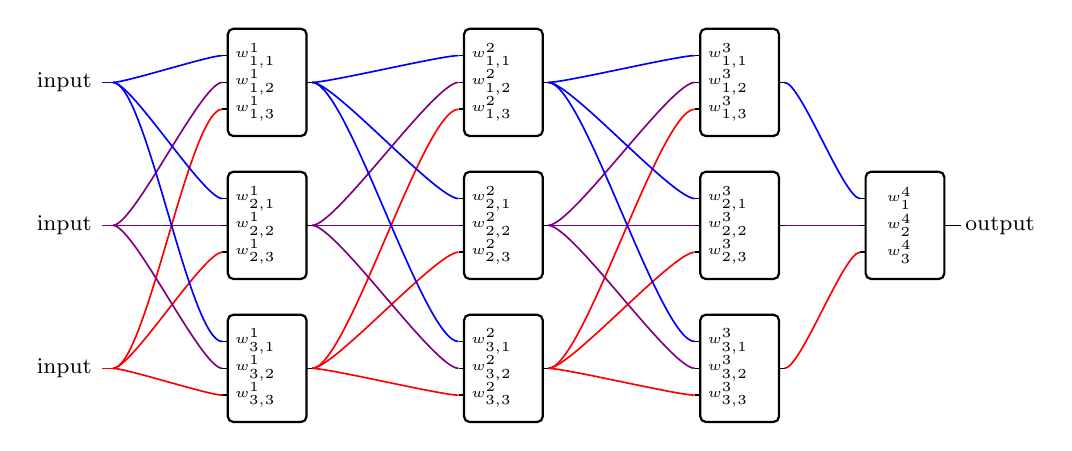
\begin{tikzpicture}[oriented WD, bb port sep=1.5, scale=2, bb port length=1pt]
	\tikzmath{
	int \hidden, \depth, \hiddeninc, \incsqrd;
	\hidden=3; %Set this
	\depth=3;  %Set this
	\hiddeninc=\hidden+1;
	\incsqrd = \hiddeninc*\hiddeninc;
	}
	\foreach \j[evaluate=\j as \col using (\j-1)/(\depth-1)*100] in {1,...,\depth} {
			\coordinate (N0\j) at (0.3,\incsqrd-\hiddeninc*\j);
			\draw[color=red!\col!blue] (N0\j) to node[coordinate, pos=1] (N0\j_out1) {} +(2pt,0);
			\node[left=0 of N0\j, font=\footnotesize] {input};
		}
	\foreach \i [remember=\i as \lasti (initially 0)] in {1,...,\hidden} {
		\foreach \j in {1,...,\depth} {
			\node[bb={\depth}{1}] (N\i\j) at (\i,\incsqrd-\hiddeninc*\j) {};
			\foreach \jj[evaluate=\jj as \col using (\jj-1)/(\depth-1)*100] in {1,...,\depth} {
				\draw[color=red!\col!blue] (N\lasti\jj_out1) to[looseness=0.3] (N\i\j_in\jj);
				\node [right=1pt, font=\tiny] at (N\i\j_in\jj) {$w^\i_{\j,\jj}$};
			}
		}
	}
	\node[bb={\depth}{1}] (N\hiddeninc) at (\hidden+.7,\incsqrd-2*\hiddeninc) {};
	\foreach \jj[evaluate=\jj as \col using (\jj-1)/(\depth-1)*100] in {1,...,\depth} {
		\draw[color=red!\col!blue] (N\hidden\jj_out1) to[looseness=0.3] (N\hiddeninc_in\jj);
		\node [right=6pt, font=\tiny] at (N\hiddeninc_in\jj) {$w^\hiddeninc_{\jj}$};
	}
	\draw (N\hiddeninc_out1) to node[right, font=\footnotesize] {output} +(2pt,0);
\end{tikzpicture}
\end{equation}



\clearpage
% Section %
\section{Tracing}

\subsection{No splitting}

\begin{equation}\label{gather and parse}\tag{gather and parse}
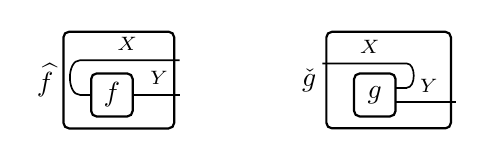
\begin{tikzpicture}[oriented WD, bbx=1em, bby=1ex, bb min width=1.5em]
	\node[bb={1}{1}] (f) {$f$};
	\node[bb={0}{0}, fit={(f.south west) ($(f.north east)+(.5,2.5)$)}] (fhat) {};
	\coordinate (fhat_out2) at (f_out1-|fhat.east);
	\coordinate (fhat_out1) at ($(fhat_out2)!.55!(fhat.north east)$);
	\begin{scope}[shorten >=-2pt]
  	\draw (f_out1) to node[above, font=\scriptsize] {$Y$} (fhat_out2);
  	\draw let \p1=(f_in1|-fhat_out1) in
  		(f_in1) to[in=180, out=180] (\x1,\y1) to node[above, font=\scriptsize] {$X$} (fhat_out1);
	\end{scope}
	\node[left=0 of fhat.west] {$\widehat{f}\coloneqq$};
%
	\node[bb port sep=1.2, bb={0}{2}, right=8 of f] (g) {$g$};
	\node[bb={0}{0}, fit={(g.south west) ($(g.north east)+(1,2.5)$)}] (ghat) {};	
	\coordinate (ghat_out2) at (g_out2-|ghat.east);
	\coordinate (ghat_in2fake) at (ghat_out2-|ghat.west);
	\coordinate (ghat_in1) at ($(ghat_in2fake)!.55!(ghat.north west)$);	
	\begin{scope}[shorten >=-2pt]
  	\draw (g_out2) to node[above, font=\scriptsize] {$Y$} (ghat_out2);
  	\draw let \p1=(g_out1|-ghat_in1) in
  		(g_out1) to[in=0, out=0] (\x1,\y1) to[in=180,out=180] node[above, font=\scriptsize, pos=.3] {$X$} (ghat_in1);
	\end{scope}
	\node[left=0 of ghat.west] {$\check{g}\coloneqq$};
\end{tikzpicture}
\end{equation}

\begin{equation}\label{minimal_feedback}\tag{minimal with feedback}
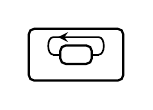
\begin{tikzpicture}[oriented WD, bb small]
	\node[bb={1}{1}] (X) {};
	\node[bb={0}{0},fit={($(X.north west)+(0,1)$) ($(X.south east)+(0,-1)$)}] (Y){};
	\draw[ar] let \p1=(X.north west), \p2=(X.north east), \n1=\bbportlen, \n2={\y1+\bby} in
		(X_out1) to[in=0] (\x2+\n1,\n2) -- (\x1-\n1,\n2) to[out=180] (X_in1);
\end{tikzpicture}
\end{equation}


\begin{equation}\label{f_and_g}\tag{f and g}
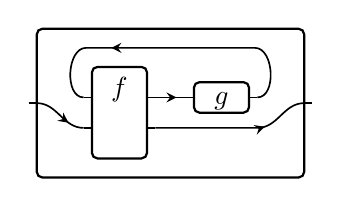
\begin{tikzpicture}[oriented WD, bb min width =.7cm, bby=1.6ex, bbx=.7cm,bb port length=3pt] 
  \node[bb port sep=1.6, bb={2}{2}, bb name=$f$] (X1) {};
  \node[bb port sep=.8,bb={1}{1}, right=.7 of X1_out1, bb name=$g$] (X2) {};
  \node[bb={1}{1}, fit={(X1) (X2) ($(X1.north)+(0,1)$)}] (Y) {};
  \draw[ar] (Y_in1') to (X1_in2);
  \draw[ar,pos=.8] (X1_out1) to (X2_in1);
  \draw[ar] let \p1=(X2.south east), \n1={\y1-.8*\bby}, \n2=\bbportlen in
          (X1_out2) -- (\x1+\n2,\n1) to (Y_out1');
  \draw[ar] let \p1=(X2.north east), \p2=(X1.north west), \n1={\y2+\bby}, \n2=\bbportlen in
          (X2_out1) to[in=0] (\x1+.7*\n2,\n1) -- (\x2-.7*\n2,\n1) to[out=180] (X1_in1);
\end{tikzpicture}
\end{equation}

\begin{equation}\label{little_trace}\tag{little trace}
	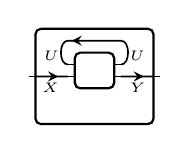
\begin{tikzpicture}[oriented WD,bb port sep=1, bb port length=2.5pt, bbx=.5cm, bb min width=.5cm, bby=1ex]
		\node[bb={2}{2}] (dom) {};
		\node[bb={1}{1}, fit={(dom) ($(dom.north)+(0,1)$) ($(dom.south)-(0,2)$)}] (cod) {};
		\draw[ar,pos=20] (cod_in1') to (dom_in2);
		\draw[ar,pos=2] (dom_out2) to (cod_out1');
		\draw[ar] let \p1=(dom.north east), \p2=(dom.north west), \n1={\y2+\bby}, \n2=\bbportlen in (dom_out1) to[in=0] (\x1+\n2,\n1) -- (\x2-\n2,\n1) to[out=180] (dom_in1);
		\draw[label] 
			node[below left=2pt and 3pt of dom_in2]{\tiny$X$}
			node[below right=2pt and 3pt of dom_out2]{\tiny$Y$}
			node[above left=1pt and 3pt of dom_in1] {\tiny$U$}
			node[above right=1pt and 3pt of dom_out1] {\tiny$U$};
	\end{tikzpicture}
\end{equation}

\begin{equation}\label{bigger_trace}\tag{bigger trace}
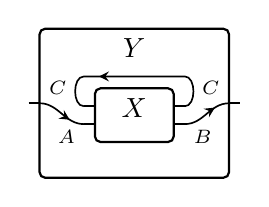
\begin{tikzpicture}[oriented WD, bbx=1em, bby=1ex]
	\node[bb={2}{2}, bb name=$X$] (dom) {};
	\node[bb={1}{1}, fit={(dom) ($(dom.north east)+(1,4)$) ($(dom.south west)-(1,2)$)}, bb name = $Y$] (cod) {};
	\draw[ar,pos=20] (cod_in1') to (dom_in2);
	\draw[ar,pos=2] (dom_out2) to (cod_out1');
	\draw[ar] let \p1=(dom.north east), \p2=(dom.north west), \n1={\y2+\bby}, \n2=\bbportlen in (dom_out1) to[in=0] (\x1+\n2,\n1) -- (\x2-\n2,\n1) to[out=180] (dom_in1);
	\draw[label] 
		node[below left=2pt and 3pt of dom_in2]{$A$}
		node[below right=2pt and 3pt of dom_out2]{$B$}
		node[above left=4pt and 6pt of dom_in1] {$C$}
		node[above right=4pt and 6pt of dom_out1] {$C$};
\end{tikzpicture}
\end{equation}

\begin{align}\label{dia:series_parallel}\tag{series parallel}
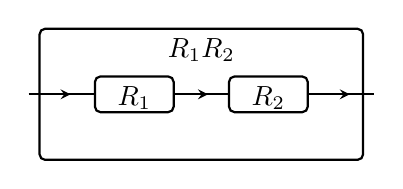
\begin{tikzpicture}[oriented WD, baseline=(Y.center), bbx=1em, bby=1ex]
	\node[bb={1}{1},bb name=$R_1$] (X1) {};
	\node[bb={1}{1},right =2 of X1, bb name=$R_2$] (X2) {};
	\node[bb={1}{1}, fit={($(X1.north west)+(-1,3)$) ($(X1.south)+(0,-3)$) ($(X2.east)+(1,0)$)}, bb name = $R_1R_2$] (Y) {};
%
	\draw[ar] (Y_in1') to (X1_in1);
	\draw[ar] (X1_out1) to (X2_in1);
	\draw[ar] (X2_out1) to (Y_out1');
\end{tikzpicture}
\qquad\qquad
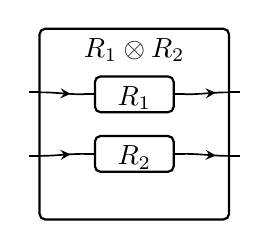
\begin{tikzpicture}[oriented WD,baseline=(Y.center), bbx=1em, bby=1ex]
	\node[bb={1}{1},bb name=$R_1$] (X1) {};
	\node[bb={1}{1},below =2 of X1, bb name=$R_2$] (X2) {};
	\node[bb={2}{2}, fit={($(X1.north west)+(-1,3)$) ($(X2.south)+(0,-3)$) ($(X2.east)+(1,0)$)}, bb name = $R_1\otimes R_2$] (Y) {};
%
	\draw[ar] (Y_in1') to (X1_in1);
	\draw[ar] (Y_in2') to (X2_in1);
	\draw[ar] (X1_out1) to (Y_out1');
	\draw[ar] (X2_out1) to (Y_out2');
\end{tikzpicture}
\qquad\qquad
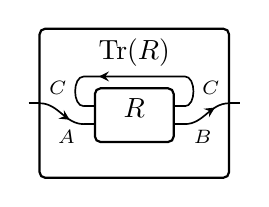
\begin{tikzpicture}[oriented WD,baseline=(cod.center), bbx=1em, bby=1ex]
	\node[bb={2}{2}, bb name=$R$] (dom) {};
	\node[bb={1}{1}, fit={(dom) ($(dom.north east)+(1,4)$) ($(dom.south west)-(1,2)$)}, bb name = $\tn{Tr}(R)$] (cod) {};
	\draw[ar,pos=20] (cod_in1') to (dom_in2);
	\draw[ar,pos=2] (dom_out2) to (cod_out1');
	\draw[ar] let \p1=(dom.north east), \p2=(dom.north west), \n1={\y2+\bby}, \n2=\bbportlen in (dom_out1) to[in=0] (\x1+\n2,\n1) -- (\x2-\n2,\n1) to[out=180] (dom_in1);
	\draw[label] 
		node[below left=2pt and 3pt of dom_in2]{$A$}
		node[below right=2pt and 3pt of dom_out2]{$B$}
		node[above left=4pt and 6pt of dom_in1] {$C$}
		node[above right=4pt and 6pt of dom_out1] {$C$};
\end{tikzpicture}
\end{align}

\begin{equation}\label{relations1}\tag{Relations 1}
	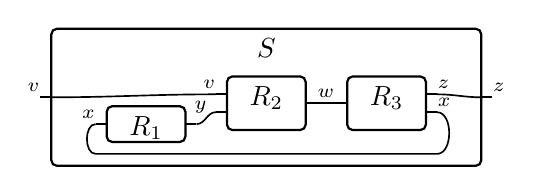
\begin{tikzpicture}[oriented WD, bbx=1em, bby=1ex]
		\node[bb={1}{1},bb name=$R_1$] (R1) {};
 		\node[bb={2}{1}, above right = -2 and 1.5 of R1, bb name=$R_2$] (R2) {};
		\node[bb={1}{2}, right = 1.5 of R2, bb name=$R_3$] (R3) {};
		\node[bb={1}{1}, fit={($(R1.south west)+(-1,-1)$) (R2) ($(R3.north east)+(1,3)$)}, bb name = $S$] (S) {};
		%
		\draw (S_in1') to (R2_in1);
		\draw (R1_out1) to (R2_in2);
		\draw (R2_out1) to (R3_in1);
		\draw (R3_out1) to (S_out1');
		\draw let \p1=(R3.south east), \p2=(R1.south west), \n1={\y2-\bby}, \n2=\bbportlen in
			(R3_out2) to[in=0] (\x1+\n2,\n1) -- (\x2-\n2,\n1) to[out=180] (R1_in1);
	%
		\draw [label]
			node[above left=.4 and 0 of R1_in1] {$x$}
			node[above right=.8 and -.1 of R1_out1] {$y$}
			node[above left=.4 and 0 of R2_in1] {$v$}
			node[above left=.4 and 0 of S_in1] {$v$}
			node[above right=.4 and 0 of R2_out1] {$w$}
			node[above right=.4 and 0 of R3_out1] {$z$}
			node[above right=.4 and 0 of S_out1] {$z$}
			node[above right=.4 and 0 of R3_out2] {$x$}
		;			
	\end{tikzpicture}
\end{equation}

\begin{equation}\label{relations2}\tag{relations 2}
	\begin{tikzpicture}[oriented WD, bbx=1em, bby=1ex]
 		\node[bb port sep=3,bb={1}{2}, bb name=$R'_2$] (R2) {};
		\node[bb port sep=1.5, bb={1}{1}, right=1 of R2_out2] (R1) {$R'_1$};
		\node[bb port sep=3,bb={2}{1}, right=5.5 of R2, bb name=$R'_3$] (R3) {};
		\node[bb={1}{1}, fit={(R1) (R2) (R3)}, bb name = $S$] (S) {};
		%
		\draw (S_in1') to (R2_in1);
		\draw (R2_out2) to (R1_in1);
		\draw (R2_out1) to (R3_in1);
		\draw (R3_out1) to (S_out1');
		\draw (R1_out1) to (R3_in2);
		%
		\draw [label]
			node[above right=.4 and 0 of R2_out2] {$y$}
			node[above right=.4 and 0 of R1_out1] {$x$}
			node[above left=.4 and 0 of R2_in1] {$v$}
			node[above right=.4 and 0 of R2_out1] {$w$}
			node[above right=.4 and 0 of R3_out1] {$z$}
		;			
	\end{tikzpicture}
\end{equation}

\begin{equation}\label{smallNestingPic}\tag{SmallNestingPic}
\begin{tikzpicture}[oriented WD, bb min width =.5cm, bbx=.5cm, bb port sep =1,bb port length=.08cm, bby=.14cm]
\path (0,0) pic {SmallNestingPic};
\end{tikzpicture}
\end{equation}


\begin{equation}\label{Zcombined}\tag{Zcombined}
\begin{tikzpicture}[oriented WD, bb min width =.5cm, bbx=.5cm, bb port sep =1,bb port length=.08cm, bby=.15cm]
\path (0,0) pic {Zcombined};
\end{tikzpicture}
\end{equation}

\begin{equation}\label{two_modules}\tag{two modules}
\begin{tikzpicture}[oriented WD, bbx=1em, bby=1ex]
 \node[bb={3}{2},bb name=$X_1$] (X1) {};
 \node[bb={2}{2},below right = -3 and 2 of X1, bb name=$X_2$] (X2) {};
 \node[bb={3}{2}, fit={($(X1.north west)+(-1,2)$) ($(X2.south)+(0,-2)$) ($(X2.east)+(1,0)$)}, bb name = $Y$] (Y) {};
%
 \draw[ar] (Y_in1') to (X1_in1);
 \draw[ar] (X1_out2) to (X2_in1);
 \draw[ar] (Y_in2') to (X1_in2);
 \draw[ar] (X1_out1) to (Y_out1');
 \draw (X2_out1) to (Y_out2');
%
 \draw[ar] let \p1=(X2.south east), \p2=(X1.south west), \n1={\y1-\bby}, \n2=\bbportlen in
 (X2_out2) to[in=0] (\x1+\n2,\n1) -- (\x2-\n2,\n1) to[out=180] (X1_in3);
 \draw[ar] let \p1=(X1.south west), \p2=(X1.south east), \n1={\y1-\bby}, \n2=\bbportlen in
 (Y_in3') to (\x1-\n2,\n1) -- (\x2-\n2,\n1) to (X2_in2);
\end{tikzpicture}
\end{equation}

\begin{equation}\label{pretty}\tag{pretty}
\begin{tikzpicture}[oriented WD, bb min width =.5cm, bbx=.5cm, bb port sep =1,bb port length=.08cm, bby=.15cm]
	\node[bb={2}{2},green!25!black,bb name = {\tiny$X_1$}] (X11) {};
	\node[bb={3}{3},green!25!black,below right=of X11,bb name = {\tiny$X_2$}] (X12) {};
	\node[bb={2}{1}, green!25!black,above right=of X12,bb name = {\tiny$X_3$}] (X13) {};
	\draw (X11_out1) to (X13_in1);
	\draw (X11_out2) to (X12_in1);
	\draw (X12_out1) to (X13_in2);

	\node[bb={2}{2}, green!25!black, below right = -1 and 1.5 of X12, bb name = {\tiny$X_4$}] (X21) {};
	\node[bb={1}{2}, green!25!black, above right=-1 and 1 of X21,bb name = {\tiny$X_5$}] (X22) {};
	\draw (X21_out1) to (X22_in1);
	\draw let \p1=(X22.north east), \p2=(X21.north west), \n1={\y1+\bby}, \n2=\bbportlen in
          (X22_out1) to[in=0] (\x1+\n2,\n1) -- (\x2-\n2,\n1) to[out=180] (X21_in1);
        
        \node[bb={2}{2}, fit = {($(X11.north east)+(-1,3)$) (X12) (X13) ($(X21.south)$) ($(X22.east)+(.5,0)$)}, bb name ={\scriptsize $Y$}] (Z) {};
	\draw (Z_in1') to (X11_in2);	
	\draw (Z_in2') to (X12_in2);
	\draw (X12_out2) to (X21_in2);
	\draw let \p1=(X22.south east),\n1={\y1-\bby}, \n2=\bbportlen in
	  (X21_out2) to (\x1+\n2,\n1) to (Z_out2');
	 \draw let \p1=(X12.south east), \p2=(X12.south west), \n1={\y1-\bby}, \n2=\bbportlen in
	  (X12_out3) to[in=0] (\x1+\n2,\n1) -- (\x2-\n2,\n1) to[out=180] (X12_in3);
	\draw let \p1=(X22.north east), \p2=(X11.north west), \n1={\y2+\bby}, \n2=\bbportlen in
          (X22_out2) to[in=0] (\x1+\n2,\n1) -- (\x2-\n2,\n1) to[out=180] (X11_in1);
	\draw let \p1=(X13_out1), \p2=(X22.north east), \n2=\bbportlen in
	 (X13_out1) to (\x1+\n2,\y1) -- (\x2+\n2,\y1) to (Z_out1');
\end{tikzpicture}
\end{equation}

\begin{equation}\label{prettier?}\tag{prettier?}
\begin{tikzpicture}[oriented WD, bb min width =.5cm, bbx=.5cm, bb port sep =1,bb port length=0, bby=.15cm]
	\node[bb={2}{2}, green!25!black, bb name = {\tiny$X_1$}] (X11) {};
	\node[bb={3}{3}, green!25!black, below right=of X11, bb name = {\tiny$X_2$}] (X12) {};
	\node[bb={2}{1}, green!25!black, above right=of X12, bb name = {\tiny$X_3$}] (X13) {};
	\node[bb={2}{2}, green!25!black, below right = -1 and 1.5 of X12, bb name = {\tiny$X_4$}] (X21) {};
	\node[bb={1}{2}, green!25!black, above right=-1 and 1 of X21,bb name = {\tiny$X_5$}] (X22) {};
  \node[bb={2}{2}, fit = {($(X11.north east)+(-1,2)$) (X12) (X13) ($(X21.south)$) ($(X22.east)+(.5,0)$)}] (Z) {};
	\draw (X21_out1) to (X22_in1);
	\draw let \p1=(X22.north east), \p2=(X21.north west), \n1={\y1+\bby}, \n2=\bbportlen in
          (X22_out1) to[in=0] (\x1+\n2,\n1) -- (\x2-\n2,\n1) to[out=180] (X21_in1);
	\draw (X11_out1) to (X13_in1);
	\draw (X11_out2) to (X12_in1);
	\draw (X12_out1) to (X13_in2);
	\draw (Z_in1'|-X11_in2) to (X11_in2);	
	\draw (Z_in2'|-X12_in2) to (X12_in2);
	\draw (X12_out2) to (X21_in2);
	\draw (X21_out2) to (Z_out2'|-X21_out2);
	 \draw let \p1=(X12.south east), \p2=(X12.south west), \n1={\y1-\bby}, \n2=\bbportlen in
	  (X12_out3) to[in=0] (\x1+\n2,\n1) -- (\x2-\n2,\n1) to[out=180] (X12_in3);
	\draw let \p1=(X22.north east), \p2=(X11.north west), \n1={\y2+\bby}, \n2=\bbportlen in
          (X22_out2) to[in=0] (\x1+\n2,\n1) -- (\x2-\n2,\n1) to[out=180] (X11_in1);
	\draw (X13_out1) to (Z_out1'|-X13_out1);
\end{tikzpicture}
\end{equation}

\begin{equation}\label{prettier no num}\tag{prettier no num}
\begin{tikzpicture}[oriented WD, bb min width =.5cm, bbx=.5cm, bb port sep =1,bb port length=0, bby=.15cm]
	\node[bb={2}{2}, green!25!black] (X11) {};
	\node[bb={3}{3}, green!25!black, below right=of X11] (X12) {};
	\node[bb={2}{1}, green!25!black, above right=of X12] (X13) {};
	\node[bb={2}{2}, green!25!black, below right = -1 and 1.5 of X12] (X21) {};
	\node[bb={1}{2}, green!25!black, above right=-1 and 1 of X21] (X22) {};
  \node[bb={2}{2}, fit = {($(X11.north east)+(-1,2)$) (X12) (X13) ($(X21.south)$) ($(X22.east)+(.5,0)$)}] (Z) {};
	\draw (X21_out1) to (X22_in1);
	\draw let \p1=(X22.north east), \p2=(X21.north west), \n1={\y1+\bby}, \n2=\bbportlen in
          (X22_out1) to[in=0] (\x1+\n2,\n1) -- (\x2-\n2,\n1) to[out=180] (X21_in1);
	\draw (X11_out1) to (X13_in1);
	\draw (X11_out2) to (X12_in1);
	\draw (X12_out1) to (X13_in2);
	\draw (Z_in1'|-X11_in2) to (X11_in2);	
	\draw (Z_in2'|-X12_in2) to (X12_in2);
	\draw (X12_out2) to (X21_in2);
	\draw (X21_out2) to (Z_out2'|-X21_out2);
	 \draw let \p1=(X12.south east), \p2=(X12.south west), \n1={\y1-\bby}, \n2=\bbportlen in
	  (X12_out3) to[in=0] (\x1+\n2,\n1) -- (\x2-\n2,\n1) to[out=180] (X12_in3);
	\draw let \p1=(X22.north east), \p2=(X11.north west), \n1={\y2+\bby}, \n2=\bbportlen in
          (X22_out2) to[in=0] (\x1+\n2,\n1) -- (\x2-\n2,\n1) to[out=180] (X11_in1);
	\draw (X13_out1) to (Z_out1'|-X13_out1);
\end{tikzpicture}
\end{equation}

\begin{equation}\label{pretty_no_num}\tag{pretty-no-num}
\begin{tikzpicture}[oriented WD, bb min width =.5cm, bbx=.5cm, bb port sep =1,bb port length=.08cm, bby=.15cm]
	\node[bb={2}{2},green!25!black] (X11) {};
	\node[bb={3}{3},green!25!black,below right=of X11] (X12) {};
	\node[bb={2}{1}, green!25!black,above right=of X12] (X13) {};
	\draw (X11_out1) to (X13_in1);
	\draw (X11_out2) to (X12_in1);
	\draw (X12_out1) to (X13_in2);

	\node[bb={2}{2}, green!25!black, below right = -1 and 1.5 of X12] (X21) {};
	\node[bb={1}{2}, green!25!black, above right=-1 and 1 of X21] (X22) {};
	\draw (X21_out1) to (X22_in1);
	\draw let \p1=(X22.north east), \p2=(X21.north west), \n1={\y1+\bby}, \n2=\bbportlen in
          (X22_out1) to[in=0] (\x1+\n2,\n1) -- (\x2-\n2,\n1) to[out=180] (X21_in1);
        
        \node[bb={2}{2}, fit = {($(X11.north east)+(-1,3)$) (X12) (X13) ($(X21.south)$) ($(X22.east)+(.5,0)$)}] (Z) {};
	\draw (Z_in1') to (X11_in2);	
	\draw (Z_in2') to (X12_in2);
	\draw (X12_out2) to (X21_in2);
	\draw let \p1=(X22.south east),\n1={\y1-\bby}, \n2=\bbportlen in
	  (X21_out2) to (\x1+\n2,\n1) to (Z_out2');
	 \draw let \p1=(X12.south east), \p2=(X12.south west), \n1={\y1-\bby}, \n2=\bbportlen in
	  (X12_out3) to[in=0] (\x1+\n2,\n1) -- (\x2-\n2,\n1) to[out=180] (X12_in3);
	\draw let \p1=(X22.north east), \p2=(X11.north west), \n1={\y2+\bby}, \n2=\bbportlen in
          (X22_out2) to[in=0] (\x1+\n2,\n1) -- (\x2-\n2,\n1) to[out=180] (X11_in1);
	\draw let \p1=(X13_out1), \p2=(X22.north east), \n2=\bbportlen in
	 (X13_out1) to (\x1+\n2,\y1) -- (\x2+\n2,\y1) to (Z_out1');
\end{tikzpicture}
\end{equation}

\begin{equation}\label{cobordism_equation}\tag{cobordism equation}
	\begin{tikzpicture}[oriented WD, bb min width =.7cm, bby=1.6ex, bbx=.7cm,bb port length=3pt,baseline=(current bounding box.center)] 
		\node[bb port sep=1.6, bb={2}{2}, bb name=$f$] (X1) {};
		\node[bb port sep=.8,bb={1}{1}, right=.7 of X1_out1, bb name=$g$] (X2) {};
		\node[bb={1}{1}, fit={(X1) (X2) ($(X1.north)+(0,1)$)}] (Y) {};
		\draw[ar] (Y_in1') to (X1_in2);
		\draw[ar,pos=.8] (X1_out1) to (X2_in1);
		\draw[ar] let \p1=(X2.south east), \n1={\y1-.8*\bby}, \n2=\bbportlen in 
			(X1_out2) -- (\x1+\n2,\n1) to (Y_out1');
		\draw[ar] let \p1=(X2.north east), \p2=(X1.north west), \n1={\y2+\bby}, \n2=\bbportlen in
			(X2_out1) to[in=0] (\x1+.7*\n2,\n1) -- (\x2-.7*\n2,\n1) to[out=180] (X1_in1);
	\end{tikzpicture}
\quad
=
\quad
	\begin{tikzpicture}[oriented WD, bb min width =.7cm, bby=1.6ex, bbx=.7cm,bb port length=3pt,baseline=(current bounding box.center)] 
		\node[bb port sep=1.6, bb={2}{2}, bb name=$f$] (X1) {};
		\node[bb port sep=.8,bb={1}{1}, left=.7 of X1_in1, bb name=$g$] (X2) {};
		\node[bb={1}{1}, fit={(X2) (X1) ($(X1.north)+(0,1)$)}] (Y) {};
		\draw[ar] (X1_out2) to (Y_out1');
		\draw[ar,pos=.8] (X2_out1) to (X1_in1);
		\draw[ar] let \p1=(X2.south west), \n1={\y1-.8*\bby}, \n2=\bbportlen in
			(Y_in1') to (\x1-\n2,\n1) -- (X1_in2);
		\draw[ar] let \p1=(X2.north west), \p2=(X1.north east), \n1={\y2+\bby}, \n2=\bbportlen in
			(X1_out1) to[in=0] (\x2+.7*\n2,\n1) -- (\x1-.7*\n2,\n1) to[out=180] (X2_in1);
	\end{tikzpicture}
\end{equation}

\begin{equation}\label{cobordism}\tag{cobordism}
\parbox{2in}{
\begin{tikzpicture}[oriented WD, bb min width =.7cm, bby=1.2ex, bbx=1.1cm,bb port length=3pt,
	label/.append style={node distance=1pt and -3pt}] 
  \node[bb={2}{1},, bb name={\tiny $X_1$}] (X1) {};
  \node[bb={1}{2}, right=.7 of X1_out1, bb name={\tiny $X_2$}] (X2) {};
  \node[bb={0}{0}, fit={(X1) (X2) ($(X1.south)-(0,3)$) ($(X1.north)+(0,5)$)}, bb name={\footnotesize$Y$}] (Y) {};
  \coordinate (Y_in1') at (Y.west|-X1_in2);
  \coordinate (Y_in2') at ($(Y_in1')-(0,20pt)$);
  \coordinate (Y_out1') at (Y.east|-X2_out2);
  \coordinate (Y_out2') at (Y.east|-Y_in2');
  \draw (Y_in1') to[in looseness=1.25] (X1_in2);
  \draw[ar,pos=.8] (X1_out1) to (X2_in1);
  \draw (X2_out2) to[out looseness=1.25] (Y_out1');
  \draw[ar] (Y_in2') -- (Y_out2');
  \draw[ar] let \p1=(X2.north east), \p2=(X1.north west), \n1={\y2+2*\bby}, \n2=\bbportlen in
   	(X2_out1) to[in=0, looseness=1.5] (\x1+.7*\n2,\n1) -- (\x2-.7*\n2,\n1) to[out=180, looseness=1.5] (X1_in1);
  \draw[label] 
        node[above left=2pt and -3pt of X1_in1] {\tiny$X_{1a}$}
        node[below left=of X1_in2] {\tiny$X_{1b}$}
        node[above right=of X1_out1] {\tiny$X_{1c}$}
        node[above left=of X2_in1] {\tiny$X_{2a}$}
        node[above right=2pt and -3pt of X2_out1] {\tiny$X_{2b}$}
        node[below right=of X2_out2] {\tiny${X}_{2c}$}
        node[left=3pt of Y_in1'] {\tiny$Y_{a}$}
        node[left=3pt of Y_in2'] {\tiny$Y_{b}$}
        node[right=3pt of Y_out1'] {\tiny$Y_{c}$}
        node[right=3pt of Y_out2'] {\tiny$Y_{d}$}
        ;

\end{tikzpicture}
}
\qquad
\parbox{1.8in}{
\begin{tikzpicture}[x=1cm,y=1ex,node distance=1 and 1,semithick,every label quotes/.style={font=\everymath\expandafter{\the\everymath\scriptstyle}},every to/.style={out=0,in=180},baseline=(current bounding box.center)]
  \node ["$X_{1a}$" left] (X1a) {$-$};
  \node [below=0 of X1a, "$X_{1b}$" left] (X1b) {$-$};
  \node [below=0 of X1b, "$X_{1c}$" left] (X1c) {$+$};
  \node [below=1.5 of X1c, "$X_{2a}$" left] (X2a) {$-$};
  \node [below=0 of X2a, "$X_{2b}$" left] (X2b) {$+$};
  \node [below=0 of X2b, "$X_{2c}$" left] (X2c) {$+$};
  \node [below right=-1 and 2 of X1a, "$Y_a$" right] (Ya) {$-$};
  \node [below=1.5 of Ya, "$Y_b$" right] (Yb) {$-$};
  \node [below=1.5 of Yb, "$Y_c$" right] (Yc) {$+$};
  \node [below=1.5 of Yc, "$Y_d$" right] (Yd) {$+$};
  \draw (X1a) to[in=0] (X2b);
  \draw (X1b) to (Ya);
  \draw (X1c) to[in=0] (X2a);
  \draw (X2c) to (Yc);
  \draw (Yb) to[out=180] (Yd);
\end{tikzpicture}
}
\end{equation}

\begin{equation}
\begin{tikzpicture}[oriented WD, bb port sep=1, bb port length=2.5pt, bb min width=.4cm, bby=.2cm, x=.5cm, y=.3cm, text height=1.5ex, text depth=.5ex]
  	\node[bb={2}{1}] (Trf) {$B_1$};
  	\node[bb={1}{1}, below=1 of Trf] (Trg) {$B_2$};
		\node[bb={2}{2}] at ($(Trf)!.5!(Trg)+(1,0)$) (Trh) {$B_3$}; 
  	\node[bb={0}{0}, fit={($(Trf.north west)+(0,1)$) (Trg) (Trh.north east)}] (Tr) {};
  	\node[coordinate] at (Tr.west|-Trf_in2) (Tr_in1) {};
  	\node[coordinate] at (Tr.west|-Trg_in1) (Tr_in2) {};
  	\node[coordinate] at (Tr.east|-Trh_out2) (Tr_out1) {};
  	\draw[shorten <=-2pt] (Tr_in1) -- (Trf_in2);
  	\draw[shorten <=-2pt] (Tr_in2) -- (Trg_in1);
  	\draw[shorten >=-2pt] (Trh_out2) -- (Tr_out1);
	\draw (Trf_out1) to (Trh_in1);
	\draw (Trg_out1) to (Trh_in2);
  	\draw let \p1=(Trh.east), \p2=(Trf.north west), \n1=\bbportlen, \n2=\bby in
  		(Trh_out1) to[in=0] (\x1+\n1,\y2+\n2) -- (\x2-\n1,\y2+\n2) to[out=180] (Trf_in1);
\end{tikzpicture}
\hspace{.5in}
\begin{tikzpicture}[decoration={brace, amplitude=5pt}, font=\tiny]
    \foreach \i in {1,...,6} {
    \node at (\i,0) (top\i) {$\bullet$};
    \node at (\i,-1) (bot\i) {$\bullet$};
    }
    \draw[decorate, thick] ($(top1)+(-.3,.2)$) -- node[above=5pt] {$B^{in}$} ($(top2)+(.3,.2)$);
    \draw[decorate, thick] ($(top3)+(-.3,.2)$) -- node[above=5pt] {$B_1^{out}$} ($(top3)+(.3,.2)$);
    \draw[decorate, thick] ($(top4)+(-.3,.2)$) -- node[above=5pt] {$B_2^{out}$} ($(top4)+(.3,.2)$);
    \draw[decorate, thick] ($(top5)+(-.3,.2)$) -- node[above=5pt] {$B_3^{out}$} ($(top6)+(.3,.2)$);
    \draw[decorate, thick] ($(bot6)+(.3,-.2)$) -- node[below=5pt] {$B^{out}$} ($(bot6)+(-.3,-.2)$);
    \draw[decorate, thick] ($(bot5)+(.3,-.2)$) -- node[below=5pt] {$B_3^{in}$} ($(bot4)+(-.3,-.2)$);
    \draw[decorate, thick] ($(bot3)+(.3,-.2)$) -- node[below=5pt] {$B_2^{in}$} ($(bot3)+(-.3,-.2)$);
    \draw[decorate, thick] ($(bot2)+(.3,-.2)$) -- node[below=5pt] {$B_1^{in}$} ($(bot1)+(-.3,-.2)$);
    \draw (top1) -- (bot2);
    \draw (top2) -- (bot3);
    \draw (top3) -- (bot4);
    \draw (top4) -- (bot5);
    \draw (top5) -- (bot6);
    \draw (top6) to[in=30, out=210] (bot1);
\end{tikzpicture}
\end{equation}

\begin{equation}\label{tensor_first}\tag{tensor first}
\begin{tikzpicture}[oriented WD,baseline=(Y.center), bbx=1em, bby=1.2ex]
 \node[bb={2}{2},bb name=$X_1$] (X1) {};
 \node[bb={2}{1},below right = -3 and 3 of X1, bb name=$X_2$] (X2) {};
 \node[bb={2}{2}, fit={($(X1.north west)+(-1,2)$) ($(X2.south)+(0,-2)$) ($(X2.east)+(1,0)$)}, bb name = $Y$] (Y) {};
%
 \draw[ar] (Y_in1') to (X1_in1);
 \draw[ar] (X1_out2) to (X2_in1);
 \draw[ar] (Y_in2') to (X2_in2);
 \draw[ar] (X1_out1) to (Y_out1');
 \draw (X2_out1) to (Y_out2');
%
 \draw[ar] let \p1=(X2.south east), \p2=(X1.south west), \n1={\y1-\bby}, \n2=\bbportlen in
 (X2_out1) to[in=0] (\x1+\n2,\n1) -- (\x2-\n2,\n1) to[out=180] (X1_in2);
 %
 \draw [label]
 	node[above left=.4 and 0 of X1_in1] {$a$}
	node[above left=.4 and 0 of X1_in2] {$b$}
	node[above left=.4 and 0 of X2_in1] {$c$}
	node[above left=.2 and 0 of X2_in2] {$d$}
	node[above right=.4 and 0 of X1_out1] {$e$}
	node[above right=.4 and 0 of X1_out2] {$f$}
	node[above right=.4 and 0 of X2_out1] {$g$}
	node[above left=.4 and 0 of Y_in1] {$h$}
	node[above left=.4 and 0 of Y_in2] {$i$}
	node[above right=.4 and 0 of Y_out1] {$j$}
	node[above right=.4 and 0 of Y_out2] {$k$};
\end{tikzpicture}
\qquad\qquad
\begin{tikzpicture}[oriented WD,baseline=(Y.center), bbx=2em, bby=1.2ex, bb port sep=1]
\begin{scope}[bbx=.25em, bb min width=.25em, bby=.5em, bb port sep=1, black!20!white]
	\node[bb={2}{2}] (X1) {$\scriptstyle X_1$};
	\node[bb={2}{1}, below =of X1] (X2) {$\scriptstyle X_2$};
\end{scope}
\node[bb={4}{3}, fit={($(X1.north)+(0,2)$) (X2)}, bb name=$X_1\boxplus X_2$] (X) {};
\begin{scope}[black!20!white]
	\draw (X_in1') to (X1_in1);
	\draw (X_in2') to (X1_in2);
	\draw (X_in3') to (X2_in1);
	\draw (X_in4') to (X2_in2);
	\draw (X1_out1) to (X_out1');
	\draw (X1_out2) to (X_out2');
	\draw (X2_out1) to (X_out3');
\end{scope}
\node[bb={2}{2}, fit={($(X.north east)+(.5,3)$) ($(X.south west)-(.5,2)$)}, bb name = $Y$] (Y) {};
%
\draw[ar] (Y_in1') to (X_in1);
\draw[ar] (Y_in2') to (X_in4);
\draw[ar] (X_out1) to (Y_out1');
\draw[ar] (X_out3) to (Y_out2');
%
\draw[ar] let \p1=(X.south east), \p2=(X.south west), \n1={\y1-\bby}, \n2=\bbportlen in
	(X_out2) to[in=0] (\x1+\n2,\n1) -- (\x2-\n2,\n1) to[out=180] (X_in3);
\draw[ar] let \p1=(X.south east), \p2=(X.south west), \n1={\y1-2*\bby}, \n2={\bbportlen} in
	(X_out3) to[in=0] (\x1+\n2,\n1) -- (\x2-\n2,\n1) to[out=180] (X_in2);	
%
\draw [label]
 	node[above left=.4 and 0 of X_in1] {$a$}
	node[above left=.4 and 0 of X_in2] {$b$}
	node[above left=.4 and 0 of X_in3] {$c$}
	node[above left=.2 and 0 of X_in4] {$d$}
	node[above right=.4 and 0 of X_out1] {$e$}
	node[above right=.4 and 0 of X_out2] {$f$}
	node[above right=.4 and 0 of X_out3] {$g$}
	node[above left=.4 and 0 of Y_in1] {$h$}
	node[above left=.4 and 0 of Y_in2] {$i$}
	node[above right=.4 and 0 of Y_out1] {$j$}
	node[above right=.4 and 0 of Y_out2] {$k$};
\end{tikzpicture}
\end{equation}

\begin{equation}\label{empty_nest}\tag{empty nest}
\begin{tikzpicture}[oriented WD, bbx = .5cm, bby =.8ex, bb min width=.5cm, bb port length=2pt, bb port sep=1]
  \node[bb={1}{3}] (X11) {};
  \node[bb={2}{1}, right=1.5 of X11] (X12) {};
  \node[bb={3}{2}, below right=of X12] (X13) {};
  \node[bb={2}{2}, fit={(X11) (X12) (X13) ($(X12.north)+(0,2)$) ($(X13.east)+(.5,0)$)}, dashed] (Y1) {};
  \node[bb={2}{1}, below left=6 and 0 of X13] (X21) {};
  \node[bb={0}{2},below left=of X21] (X22) {};
  \node[bb={1}{2}, fit=(X21) (X22), dashed] (Y2) {};
  \node[bb={2}{3}, fit={($(Y1.north)+(0,1)$) ($(Y2.south)-(0,1)$) ($(Y1.west)-(.25,0)$) ($(Y1.east)+(.25,0)$)}] (Z) {};
  \begin{scope}[gray]
  \draw[ar] (Z_in1') to (Y1_in1);
  \draw[ar] (Z_in2') to (Y2_in1);
  \draw (Y2_in1') to[in looseness=2] (X21_in1);
  \draw[ar] (X22_out1) to (X21_in2);
  \draw (X22_out2) to (Y2_out2');
  \draw[ar] (Y2_out2) to (Z_out3');
  \draw (Y1_in1') to (X11_in1);
  \draw (X13_out2) to (Y1_out2');
  \draw (Y1_in2') to[in looseness=2] (X13_in3);
  \draw (X11_out3) to[in looseness=2] (X13_in2);%
  \draw (X12_out1) to (X13_in1);
  \draw (X11_out2) to (X12_in2);
  \draw (Y1_out1) to (Z_out1');
  \draw[ar] (Y1_out2) to (Z_out2');
  \draw (X21_out1) to (Y2_out1');
  \draw[ar] let \p1=(Y2.north east), \p2=(Y1.south west), \n1={\y1+2*\bby}, \n2=\bbportlen in
  	(Y2_out1) to[in=0] (\x1+\n2,\n1) -- (\x2-\n2,\n1) to[out=180] (Y1_in2);
  \draw[ar] let \p1=(X13.north east), \p2=(X12.north west), \n1={\y2+\bby}, \n2=\bbportlen in
  	(X13_out1) to[in=0] (\x1+\n2,\n1) -- (\x2-\n2,\n1) to[out=180] (X12_in1);
  \draw let \p1=(X12.north west), \p2=(X13.north east), \n1={\y1+2*\bby}, \n2=\bbportlen in
  	(X11_out1) to (\x1-2*\n2,\n1) -- (\x2+2*\n2,\n1) to[out=0] (Y1_out1');
  \end{scope}
  \end{tikzpicture}
\end{equation}

\begin{equation}\label{empty_nest_red_egg}\tag{empty nest red egg}
\begin{tikzpicture}[oriented WD, bbx = .5cm, bby =.8ex, bb min width=.5cm, bb port length=2pt, bb port sep=1]
  \node[bb={1}{3}] (X11) {};
  \node[bb={2}{1}, right=1.5 of X11] (X12) {};
  \node[bb={3}{2}, red, below right=of X12] (X13) {};
  \node[bb={2}{2}, fit={(X11) (X12) (X13) ($(X12.north)+(0,2)$) ($(X13.east)+(.5,0)$)}, dashed] (Y1) {};
  \node[bb={2}{1}, below left=6 and 0 of X13] (X21) {};
  \node[bb={0}{2},below left=of X21] (X22) {};
  \node[bb={1}{2}, fit=(X21) (X22), dashed] (Y2) {};
  \node[bb={2}{3}, fit={($(Y1.north)+(0,1)$) ($(Y2.south)-(0,1)$) ($(Y1.west)-(.25,0)$) ($(Y1.east)+(.25,0)$)}] (Z) {};
  \begin{scope}[gray]
  \draw[ar] (Z_in1') to (Y1_in1);
  \draw[ar] (Z_in2') to (Y2_in1);
  \draw (Y2_in1') to[in looseness=2] (X21_in1);
  \draw[ar] (X22_out1) to (X21_in2);
  \draw (X22_out2) to (Y2_out2');
  \draw[ar] (Y2_out2) to (Z_out3');
  \draw (Y1_in1') to (X11_in1);
  \draw (X13_out2) to (Y1_out2');
  \draw (Y1_in2') to[in looseness=2] (X13_in3);
  \draw (X11_out3) to[in looseness=2] (X13_in2);%
  \draw (X12_out1) to (X13_in1);
  \draw (X11_out2) to (X12_in2);
  \draw (Y1_out1) to (Z_out1');
  \draw[ar] (Y1_out2) to (Z_out2');
  \draw (X21_out1) to (Y2_out1');
  \draw[ar] let \p1=(Y2.north east), \p2=(Y1.south west), \n1={\y1+2*\bby}, \n2=\bbportlen in
  	(Y2_out1) to[in=0] (\x1+\n2,\n1) -- (\x2-\n2,\n1) to[out=180] (Y1_in2);
  \draw[ar] let \p1=(X13.north east), \p2=(X12.north west), \n1={\y2+\bby}, \n2=\bbportlen in
  	(X13_out1) to[in=0] (\x1+\n2,\n1) -- (\x2-\n2,\n1) to[out=180] (X12_in1);
  \draw let \p1=(X12.north west), \p2=(X13.north east), \n1={\y1+2*\bby}, \n2=\bbportlen in
  	(X11_out1) to (\x1-2*\n2,\n1) -- (\x2+2*\n2,\n1) to[out=0] (Y1_out1');
  \end{scope}
  \end{tikzpicture}
  \end{equation}


\begin{equation}\label{two_clusters1}\tag{two clusters 1}
\begin{tikzpicture}[oriented WD, bbx = .5cm, bby =.8ex, bb min width=.5cm, bb port length=2pt, bb port sep=1]
  \node[bb={1}{3}] (X11) {$\scriptstyle X_{11}$};
  \node[bb={2}{1}, right=1.5 of X11] (X12) {$\scriptstyle X_{12}$};
  \node[bb={3}{2}, below right=of X12] (X13) {$\scriptstyle X_{13}$};
  \node[bb={2}{2}, fit={(X11) (X12) (X13) ($(X12.north)+(0,2)$) ($(X13.east)+(.5,0)$)}, dashed] (Y1) {};
  \node[bb={2}{1}, below left=6 and 0 of X13] (X21) {$\scriptstyle X_{21}$};
  \node[bb={0}{2},below left=of X21] (X22) {$\scriptstyle X_{22}$};
  \node[bb={1}{2}, fit=(X21) (X22), dashed] (Y2) {};
  \node[bb={2}{3}, fit={($(Y1.north)+(0,1)$) ($(Y2.south)-(0,1)$) ($(Y1.west)-(.25,0)$) ($(Y1.east)+(.25,0)$)}] (Z) {};
  \draw[label] 
	node at ($(Y1.north west)+(.5,-2)$)  {$Y_1$}
	node at ($(Y2.north west)+(.5,-2)$)  {$Y_2$}
	node at ($(Z.north west)+(.5,-2)$)  {$Z$};
  \begin{scope}[gray]
  \draw[ar] (Z_in1') to (Y1_in1);
  \draw[ar] (Z_in2') to (Y2_in1);
  \draw (Y2_in1') to[in looseness=2] (X21_in1);
  \draw[ar] (X22_out1) to (X21_in2);
  \draw (X22_out2) to (Y2_out2');
  \draw[ar] (Y2_out2) to (Z_out3');
  \draw (Y1_in1') to (X11_in1);
  \draw (X13_out2) to (Y1_out2');
  \draw (Y1_in2') to[in looseness=2] (X13_in3);
  \draw (X11_out3) to[in looseness=2] (X13_in2);%
  \draw (X12_out1) to (X13_in1);
  \draw (X11_out2) to (X12_in2);
  \draw (Y1_out1) to (Z_out1');
  \draw[ar] (Y1_out2) to (Z_out2');
  \draw (X21_out1) to (Y2_out1');
  \draw[ar] let \p1=(Y2.north east), \p2=(Y1.south west), \n1={\y1+2*\bby}, \n2=\bbportlen in
  	(Y2_out1) to[in=0] (\x1+\n2,\n1) -- (\x2-\n2,\n1) to[out=180] (Y1_in2);
  \draw[ar] let \p1=(X13.north east), \p2=(X12.north west), \n1={\y2+\bby}, \n2=\bbportlen in
  	(X13_out1) to[in=0] (\x1+\n2,\n1) -- (\x2-\n2,\n1) to[out=180] (X12_in1);
  \draw let \p1=(X12.north west), \p2=(X13.north east), \n1={\y1+2*\bby}, \n2=\bbportlen in
  	(X11_out1) to (\x1-2*\n2,\n1) -- (\x2+2*\n2,\n1) to[out=0] (Y1_out1');
  \end{scope}
  \end{tikzpicture}
\end{equation}

\begin{equation}\label{two_clusters2}\tag{two clusters 2}
\begin{tikzpicture}[oriented WD, bbx = .5cm, bby =.8ex, bb min width=.5cm, bb port length=2pt, bb port sep=1]
  \node[bb={1}{3}] (X11) {$X_{11}$};
  \node[bb={2}{1}, right=1.5 of X11] (X12) {$X_{12}$};
  \node[bb={3}{2}, below right=of X12] (X13) {$X_{13}$};
  \node[bb={2}{2}, fit={(X11) (X12) (X13) ($(X12.north)+(0,5)$) ($(X13.east)+(.5,0)$)}, dashed, bb name={$Y_1$}] (Y1) {};
  \node[bb={2}{1}, below left=9 and 0 of X13] (X21) {$X_{21}$};
  \node[bb={0}{2},below left=of X21] (X22) {$X_{22}$};
  \node[bb={1}{2}, fit={($(X21.north east)+(0,3)$) (X22)}, dashed, bb name={$Y_2$}] (Y2) {};
  \node[bb={2}{3}, fit={($(Y1.north)+(0,3)$) ($(Y2.south)-(0,1)$) ($(Y1.west)-(.25,0)$) ($(Y1.east)+(.25,0)$)}, bb name={$Z$}] (Z) {};
  \begin{scope}[gray]
  \draw[ar] (Z_in1') to (Y1_in1);
  \draw[ar] (Z_in2') to (Y2_in1);
  \draw (Y2_in1') to[in looseness=2] (X21_in1);
  \draw[ar] (X22_out1) to (X21_in2);
  \draw (X22_out2) to (Y2_out2');
  \draw[ar] (Y2_out2) to (Z_out3');
  \draw (Y1_in1') to (X11_in1);
  \draw (X13_out2) to (Y1_out2');
  \draw (Y1_in2') to[in looseness=2] (X13_in3);
  \draw (X11_out3) to[in looseness=2] (X13_in2);%
  \draw (X12_out1) to (X13_in1);
  \draw (X11_out2) to (X12_in2);
  \draw (Y1_out1) to (Z_out1');
  \draw[ar] (Y1_out2) to (Z_out2');
  \draw (X21_out1) to (Y2_out1');
  \draw[ar] let \p1=(Y2.north east), \p2=(Y1.south west), \n1={\y1+2*\bby}, \n2=\bbportlen in
  	(Y2_out1) to[in=0] (\x1+\n2,\n1) -- (\x2-\n2,\n1) to[out=180] (Y1_in2);
  \draw[ar] let \p1=(X13.north east), \p2=(X12.north west), \n1={\y2+\bby}, \n2=\bbportlen in
  	(X13_out1) to[in=0] (\x1+\n2,\n1) -- (\x2-\n2,\n1) to[out=180] (X12_in1);
  \draw let \p1=(X12.north west), \p2=(X13.north east), \n1={\y1+2*\bby}, \n2=\bbportlen in
  	(X11_out1) to (\x1-2*\n2,\n1) -- (\x2+2*\n2,\n1) to[out=0] (Y1_out1');
  \end{scope}
  \end{tikzpicture}
\end{equation}

\begin{equation}\label{Andrea}\tag{Andrea}
\begin{tikzpicture}[oriented WD, bb min width =.7cm, bby=1.6ex, bbx=.7cm,bb port length=3pt] 
  \node[bb port sep=.8, bb={2}{1}, bb name=$\Sigma$] (Sigma1) {};
  \node[bb port sep=1.6,bb min width=4.3em, bb={2}{3}, below right=-2.5 and 1 of Sigma1.south east, bb name=Chassis] (Chassis) {};
  \node[bb port sep=.9,bb min width=4.3em, bb={2}{4}, below right=-3 and 2 of Chassis_out2, bb name=Motor] (Motor) {};
	\node[bb port sep=.8, bb={2}{1}, right= of Motor.south east, bb name=$\Sigma$] (Sigma2) {};
  \node[bb={2}{3}, fit={($(Sigma1.north west)+(0,1)$) (Chassis) (Motor) (Sigma2)}] (Y) {};
  \draw[ar] (Y_in1') to (Sigma1_in2);
  \draw[ar] (Y_in2') to (Chassis_in2);
  \draw[ar] (Sigma1_out1) to (Chassis_in1);
  \draw[ar] (Chassis_out1) to (Motor_in1);
  \draw[ar] (Chassis_out2) to (Motor_in2);
  \draw[ar] let \p1=(Motor.south west), \p2=(Motor.south east), \n1={\y1-\bby},\n2=\bbportlen in
  	(Chassis_out3) to (\x1-\n2,\n1) -- (\x2+\n2,\n1) to (Sigma2_in2);
  \draw[ar] (Motor_out2) to (Y_out1');
  \draw[ar] (Motor_out3) to (Y_out2');
  \draw[ar] (Motor_out4) to (Sigma2_in1);
  \draw[ar] (Sigma2_out1) to (Y_out3'); 
  \draw[ar] let \p1=(Motor.north east), \p2=(Sigma1.north west), \n1={\y2+\bby},\n2=\bbportlen in
  	(Motor_out1) to[in=0] (\x1+\n2,\n1) -- (\x2-\n2,\n1) to[out=180] (Sigma1_in1);
	\draw[label]
		node[left=.3 of Y_in1] {\footnotesize Extra payload}
		node[left=.3 of Y_in2] {\footnotesize Velocity}
		node[right=.3 of Y_out1] {\footnotesize Voltage}
		node[right=.3 of Y_out2] {\footnotesize Current}
		node[right=.3 of Y_out3] {\footnotesize Cost \$}
		node[above right=.2 and 0 of Chassis_out1] {\tiny Torque}
		node[above right=.2 and 0 of Chassis_out2] {\tiny Speed}
		node[above right=.2 and 0 of Chassis_out3] {\tiny Cost \$}
		node[above right=.3 and .3 of Motor_out1, align=center, font=\tiny] {Motor\\weight}
	;	
\end{tikzpicture}
\end{equation}

\begin{equation}\label{string decoration}\tag{string decoration}
\begin{tikzpicture}
[oriented WD, bb min width =.5cm, bby=2ex, bbx=.6cm, bb port length=3pt, 
string decoration = {\node[circle, inner sep=0pt, fill=white, font=\fontsize{5}{5}\selectfont] {$\leq$};},
baseline=(Y)] 
  \node[bb port sep=.8, bb={3}{1}] (Sigma1) {$\Sigma$};
  \node[bb port sep=2,bb min width=4.3em, bb={2}{3}, below right=-3 and 1 of Sigma1.south east] (Chassis) {Chassis};
  \node (Chassis 15) at ($(Chassis_out1)!.5!(Chassis_out2)$) {};
  \node[bb port sep=2*3/5,bb min width=4.3em, bb={2}{4}, right=2 of Chassis 15] (Motor) {Motor};
  \node[bb port sep=2*3/5, bb={2}{2}, bb min width=4.3em, right=2 of Motor] (Battery) {Battery};
	\node[bb port sep=.8, bb={3}{1}, below right=-.5 and 1 of Battery] (Sigma2) {$\Sigma$};
  \node[bb={0}{0}, fit={($(Sigma1.north west)+(-.5,2)$) (Chassis) (Motor) (Sigma2)}] (Y) {};
	\node[coordinate] (Y_in1) at (Y.west|-Sigma1_in3) {};
	\node[coordinate] (Y_in2) at (Y.west|-Chassis_in2) {};
	\node[coordinate] (Y_out1) at (Y.east|-Sigma2_out1) {};
  \draw[ar] (Y_in1) to (Sigma1_in3);
  \draw[ar] (Y_in2) to (Chassis_in2);
  \draw[ar] (Sigma1_out1) to (Chassis_in1);
  \draw[ar] (Chassis_out1) to (Motor_in1);
  \draw[ar] (Chassis_out2) to (Motor_in2);
  \draw[ar] let \p1=(Motor.west), \p2=(Sigma2_in3), \n1=\bbportlen in
  	(Chassis_out3) to (\x1-\n1,\y2) -- (Sigma2_in3);
  \draw[ar] (Motor_out2) to node[above=-1pt, font=\tiny] {Voltage} (Battery_in1);
  \draw[ar] (Motor_out3) to node[above=-1pt, font=\tiny] {Current} (Battery_in2);
  \draw[ar] let \p1=(Battery.west), \p2=(Sigma2_in2), \n1=\bbportlen in
    (Motor_out4) to node[pos=.4, above=1pt, font=\tiny] {Cost \$} (\x1-\n1, \y2) -- (Sigma2_in2);
  \draw[ar] (Battery_out2) to (Sigma2_in1);
  \draw[ar, string decoration pos=.5] (Sigma2_out1) to (Y_out1); 
  \draw[ar, string decoration = {\node[circle, inner sep=0pt, fill=white, font=\fontsize{5}{5}\selectfont] {$\geq$};}, string decoration pos=.5] let \p1=(Motor.north east), \p2=(Sigma1.north west), \n1={\y2+\bby},\n2=\bbportlen in
  	(Motor_out1) to[in=0] (\x1+\n2,\n1) -- (\x2-\n2,\n1) to[out=180] (Sigma1_in1);
  \draw[ar, string decoration = {\node[circle, inner sep=0pt, fill=white, font=\fontsize{5}{5}\selectfont] {$\geq$};}, string decoration pos=.5] let \p1=(Battery.north east), \p2=(Sigma1.north west), \n1={\y2+\bby+\bby},\n2=\bbportlen in
  	(Battery_out1) to[in=0] (\x1+\n2,\n1) -- (\x2-\n2,\n1) to[out=180] (Sigma1_in2);
%
	\draw[label]
		node[left=.3 of Y_in1] {\footnotesize Extra payload}
		node[left=.3 of Y_in2] {\footnotesize Velocity}
		node[right=.3 of Y_out1] {\footnotesize Cost \$}
		node[above right=.2 and 0 of Chassis_out1] {\tiny Torque}
		node[above right=.2 and 0 of Chassis_out2] {\tiny Speed}
		node[above right=.2 and 0 of Chassis_out3] {\tiny Cost \$}
		node[above right=.3 and .5 of Motor_out1, align=left, font=\tiny] {Motor\\Weight}
		node[above right=.3 and .8 of Battery_out1, align=left, font=\tiny] {Battery\\Weight}
		node[above right=.2 and 0 of Battery_out2, font=\tiny] {Cost \$}
	;	
\end{tikzpicture}
\end{equation}

\subsection{Diverging}

\begin{equation}\tag{kitchen sink}
\begin{tikzpicture}[oriented WD,baseline=(Y.center), bbx=2em, bby=1.2ex, bb port sep=1.2]
\node[bb={5}{5}] (X) {};
\node[bb={2}{3}, fit={($(X.north east)+(0.7,1.7)$) ($(X.south west)-(.7,.7)$)}] (Y) {};
\node [circle,minimum size=4pt, inner sep=0, fill] (dot1) at ($(Y_in1')+(.5,0)$) {};
\node [circle,minimum size=4pt, inner sep=0, fill] (dot2) at ($(X_out4)+(.5,0)$) {};
\draw[ar] (Y_in1') to (dot1);
\draw[ar] (X_out4) to (dot2);
\draw[ar] (Y_in2') to (X_in5);
\draw[ar] (Y_in2') to (X_in4);
\draw[ar] (X_out5) to (Y_out3');
\draw[ar] (X_out2) to (Y_out1');
\draw[ar] (X_out2) to (Y_out2');
%
\draw[ar] let \p1=(X.north west), \p2=(X.north east), \n1={\y1+\bby}, \n2=\bbportlen in
	(X_out1) to[in=0] (\x2+\n2,\n1) -- (\x1-\n2,\n1) to[out=180] (X_in1);
\draw[ar] let \p1=(X.north west), \p2=(X.north east), \n1={\y1+2*\bby}, \n2=\bbportlen in
	(X_out1) to[in=0] (\x2+\n2,\n1) -- (\x1-\n2,\n1) to[out=180] (X_in2);
%
\draw [label] node at ($(X.east)+(1.2,4.5)$) {$Y$}
              node at ($(X.west)+(.6,0)$) {$X$}
	      node[left=.1 of X_in3]  {$\dotso$}
	      node[right=.1 of X_out3] {$\dotso$};
\end{tikzpicture}
\end{equation}

\begin{equation}\label{kitchen sink 2}\tag{kitchen sink 2}
\begin{tikzpicture}[oriented WD, baseline=(Y.center), bb port sep=1.2, bb port length=0]
  \node[bb={6}{6}] (X) {};
  \node[bb={1}{0}, fit={($(X.north east)+(0.7,1.7)$) ($(X.south west)-(.7,.7)$)}] (Y) {};
  \node [circle, minimum size=4pt, inner sep=0, fill] (dot1) at ($(Y_in1')+(.5,0)$) {};
  \node [circle, minimum size=4pt, inner sep=0, fill] (dot2) at ($(X_in5)+(-.5,0)$) {};
  \draw[ar] (Y.west|-dot1) to (dot1);
  \draw[ar] (Y.west|-X_in6) to (X_in6);
  \draw[ar] (dot2) to (X_in5);
  \draw[ar] (X_out2) to (X_out2-|Y.east);
  \draw[ar] (X_out5) to (X_out6-|Y.east);
  \draw[ar] (X_out6) to (X_out6-|Y.east);
  %
  \draw[ar] let \p1=(X.north west), \p2=(X.north east), \n1={\y1+\bby}, \n2=\bbportlen in
  	(X_out1) to[in=0] (\x2+\n2,\n1) -- (\x1-\n2,\n1) to[out=180] (X_in1);
  \draw[ar] let \p1=(X.north west), \p2=(X.north east), \n1={\y1+2*\bby}, \n2=\bbportlen in
  	(X_out1) to[in=0] (\x2+\n2,\n1) -- (\x1-\n2,\n1) to[out=180] (X_in2);
  %
  \draw [label]
		node[left=.1 of X_in3]  {$\vdots$}
		node[right=.1 of X_out3] {$\vdots$};
	\draw[red, shorten <=-.5cm, shorten >=-.5cm] (Y.north west) -- (Y.south east);
	\draw[red, shorten <=-.5cm, shorten >=-.5cm] (Y.north east) -- (Y.south west);
\end{tikzpicture}
\end{equation}

\begin{equation}\label{simple_2}\tag{simple 2}
\begin{tikzpicture}[oriented WD, bb min width=.6cm, bb port sep=1, bbx=.6cm, bby=1ex, bb port length=2.5pt]
  \node[bb port sep=2, bb={2}{2}] (X1) {};
  \node[bb={1}{1}, right=.7 of X1_out1] (X2) {};
  \node[bb={1}{2}, fit={(X1) (X2) ($(X1.north)+(0,1)$)}] (Y) {};
  \draw[ar] (Y_in1') to (X1_in2);
  \draw[ar] (X1_out1) to (X2_in1);
  \draw (X2_out1) to[in looseness=1] (Y_out1');
  \draw[ar] (X1_out2) to (Y_out2');
  \draw[ar] let \p1=(X2.north east), \p2=(X1.north west), \n1={\y2+\bby}, \n2=\bbportlen in
          (X2_out1) to[in=0,in looseness=.9] (\x1+.7*\n2,\n1) -- (\x2-.7*\n2,\n1) to[out=180] (X1_in1);
  \end{tikzpicture}
\end{equation}

\begin{equation}\label{split_trace}\tag{split trace}
\begin{tikzpicture}[oriented WD, bbx=1em, bby=1ex]
	\node[bb={1}{1},bb name=$M_1$] (M1) {};
	\node[bb={1}{1},right=2 of M1,bb name=$M_2$] (M2) {};
	\node[bb={0}{1},fit={($(M1.north west)+(-.5,1)$) ($(M2.south east)+(.5,-1)$)}] (Y) {};
	\draw[ar] (M1_out1) to (M2_in1);
	\draw (M2_out1) to (Y_out1');
	\draw[ar] let \p1=(M2.south east), \p2=(M1.south west),\n1=\bbportlen,\n2={\y1-\bby} in
		(M2_out1) to[in=0] (\x1+\n1,\n2) -- (\x2-\n1,\n2) to[out=180] (M1_in1);
\end{tikzpicture}
\end{equation}

\begin{equation}\label{numbers}\tag{numbers}
\parbox{1.85in}{
\begin{tikzpicture}[oriented WD, bbx=1em, bby=1ex]
	\node[bb={1}{1},bb name=$M_1$] (M1) {};
	\node[bb={1}{1},right=1 of M1,bb name=$M_2$] (M2) {};
	\node[bb={1}{2},dashed, fit={(M1) (M2)}] (dashed) {};
	\node[bb={0}{1},fit={($(dashed.north west)+(-.5,1)$) ($(dashed.south east)+(.5,-1)$)}] (Y) {};
	\draw[ar] (M1_out1) to (M2_in1);
	\draw (M2_out1) to (dashed_out1');
	\draw (M2_out1) to (dashed_out2');
	\draw (dashed_in1') to (M1_in1);
	\draw (dashed_out1) to (Y_out1');
	\draw[ar] let \p1=(dashed.south east), \p2=(dashed.south west),\n1=\bbportlen,\n2={\y1-\bby} in
		(dashed_out2) to[in=0] (\x1+\n1,\n2) -- (\x2-\n1,\n2) to[out=180] (dashed_in1);
	\draw[label]
		node[above right=.5 and 0 of M1_out1] {$3$}
		node[above right=.5 and 0 of dashed_out1] {$2$}
		node[above left=.5 and 0 of M1_in1] {$2$}
	;
\end{tikzpicture}
}
\qquad
\parbox{2.1in}{
\begin{tikzpicture}[oriented WD, bbx=1em, bby=1ex]
	\node[bb={1}{1},bb name=$M_1$] (M1) {};
	\node[bb={1}{1},left=2 of M1.north west,bb name=$M_2$] (M2) {};
	\node[bb={1}{2},dashed, fit={($(M2.north west)+(-.5,2)$) ($(M1.south east)+(.5,-1)$)}] (dashed) {};
	\node[bb={0}{1},fit={($(dashed.north west)+(-.75,1)$) ($(dashed.south east)+(.75,-1)$)}] (Y) {};
	\draw[ar] (M2_out1) to (M1_in1);
	\draw[ar] (M1_out1) to (dashed_out2');
	\draw[ar] (dashed_in1') to (M2_in1);
	\draw[ar] (dashed_out1) to (Y_out1');
	\draw[ar] let \p1=(M1.north west), \p2=(dashed_out1), \n2=\bbportlen in
		(M2_out1) to (\x1-\n2,\y2) -- (dashed_out1'); 
	\draw[ar] let \p1=(dashed.south east), \p2=(dashed.south west), \n1=\bbportlen, \n2={\y1-\bby} in
		(dashed_out2) to[in=0] (\x1+\n1,\n2) -- (\x2-\n1,\n2) to[out=180] (dashed_in1);
	\draw[label]
		node[above right=.5 and .5 of M1_out1] {$3$}
		node[right=.8 of M2_out1] {$2$}
		node[above left=.5 and .1 of M2_in1] {$3$}
	;
\end{tikzpicture}
}
\qquad
\parbox{1.5in}{
\begin{tikzpicture}[oriented WD, bbx=1em, bby=1ex, bb port sep=1.3]
	\node[bb={0}{2},bb name=$M_1$] (M1) {};
	\node[bb={2}{0},right=2 of M1,bb name=$M_2$] (M2) {};
	\node[bb={0}{1},fit={($(M1.north west)+(0.5,2.5)$) ($(M2.south east)+(0.5,0)$)}] (Y) {};
	\draw (M1_out1) to (M2_in1);
	\draw[ar] (M1_out2) to (M2_in2);
	\draw[ar] let \p1=(M2.north west), \p2=(M2.north east), \n1=\bbportlen, \n2={\y1+\bby} in
		(M1_out1) to (\x1-\bbportlen,\n2) -- (\x2+\bbportlen,\n2) to (Y_out1');
	\draw[label]
		node[above right=.3 and 0 of M1_out1] {$2$}
		node[below right=.3 and 0 of M1_out2] {$3$}
	;
\end{tikzpicture}
}
\end{equation}

\begin{equation}\label{neuron1}\tag{neuron1}
\begin{tikzpicture}[oriented WD, bbx=1em, bby=1ex, bb port sep=1]
  \node[bb={2}{1}] (N1) {$\scriptstyle N_1$};
  \node[bb={1}{1}, below = 1 of N1] (N2) {$\scriptstyle N_2$};
  \node[bb={3}{1}, below=1 of N2] (N3) {$\scriptstyle N_3$};
  \node[bb={3}{1}, above right = -3 and 3.5 of N3] (N6) {$\scriptstyle N_6$};
  \node[bb={2}{1}, above =of N6] (N5) {$\scriptstyle N_5$};
  \node[bb={2}{1}, above= of N5] (N4) {$\scriptstyle N_4$};
  \node[bb={4}{4}, fit={($(N2.west)-(.5,0)$) ($(N4.north)+(0,2)$) ($(N5.east)+(1.5,0)$) ($(N3.south)-(0,1)$)}, bb name={$\scriptstyle X$}] (X) {};
  \draw (X_in1') to (N1_in2);
  \draw (X_in2') to (N2_in1);
  \draw (X_in3') to (N3_in1);
  \draw (X_in4') to (N3_in2);
  \draw (N1_out1) to (N4_in1);
  \draw (N2_out1) to (N4_in2);
  \draw (N2_out1) to (N5_in1);
  \draw (N2_out1) to (N6_in1);
  \draw (N4_out1) to (X_out1');
  \draw (N3_out1) to (N6_in2);
  \draw (N5_out1) to (X_out2');
  \draw (N6_out1) to (X_out3');
  \draw (N6_out1) to (X_out4'); 
  \draw let \p1=(N2.south east), \p2=(N3_out1),\n2=\bbportlen in
  	(N3_out1) -- (\x1+\n2,\y2) to (N5_in2);
  \draw let \p1=(N6.south east), \p2=(N3.south west), \n1={\y2-\bby}, \n2=\bbportlen in
          (N5_out1) to[in=0, looseness=.8] (\x1+\n2,\n1) -- (\x2-\n2,\n1) to[out=180] (N3_in3);
  \draw let \p1=(N6.south east), \p2=(N6.south west), \n1={\y2-\bby}, \n2=\bbportlen in
          (N6_out1) to[in=0] (\x1+\n2,\n1) -- (\x2-\n2,\n1) to[out=180] (N6_in3);
  \draw let \p1=(N1.north east), \p2=(N1.north west), \n1={\y2+\bby}, \n2=\bbportlen in
          (N1_out1) to[in=0] (\x1+\n2,\n1) -- (\x2-\n2,\n1) to[out=180] (N1_in1);
\end{tikzpicture}
\end{equation}

\begin{equation}\label{neuron2}\tag{neuron2}
\begin{tikzpicture}[oriented WD, bbx=1em, bby=1ex, bb port sep=1]
  \node[bb={3}{1}] (N0) {$\scriptstyle N_0$};
  \node[bb={3}{1}, below = 1 of N0] (N1) {$\scriptstyle N_1$};
  \node[bb={2}{1}, right= 3.5 of N0] (N2) {$\scriptstyle N_2$};
  \node[bb={3}{1}, below=1 of N1] (N3) {$\scriptstyle N_3$};
  \node[bb={2}{1}, below =of N2] (N4) {$\scriptstyle N_4$};
  \node[bb={3}{1}, below =of N4] (N5) {$\scriptstyle N_5$};
  \node[bb={7}{8}, fit={($(N1.west)-(.5,0)$) ($(N2.north)+(0,2)$) ($(N4.east)+(1.5,0)$) ($(N3.south)-(0,1)$)}, bb name={$\scriptstyle X$}] (X) {};
  \draw (X_in1') to (N0_in2);
  \draw (X_in2') to (N0_in3);
  \draw (X_in3') to (N1_in1);
  \draw (X_in4') to (N1_in2);
  \draw (X_in5') to (N1_in3);
  \draw (X_in6') to (N3_in1);
  \draw (X_in7') to (N3_in2);
  \draw (N0_out1) to (N2_in1);
  \draw (N1_out1) to (N2_in2);
  \draw (N1_out1) to (N4_in1);
  \draw (N1_out1) to (N5_in1);
  \draw (N2_out1) to (X_out1');
  \draw (N2_out1) to (X_out2');
  \draw (N2_out1) to (X_out3');
  \draw (N3_out1) to (N5_in2);
  \draw (N4_out1) to (X_out4');
  \draw (N4_out1) to (X_out5');
  \draw (N4_out1) to (X_out6');
  \draw (N5_out1) to (X_out7');
  \draw (N5_out1) to (X_out8'); 
  \draw let \p1=(N1.south east), \p2=(N3_out1),\n2=\bbportlen in
  	(N3_out1) -- (\x1+\n2,\y2) to (N4_in2);
  \draw let \p1=(N5.south east), \p2=(N3.south west), \n1={\y2-\bby}, \n2=\bbportlen in
          (N4_out1) to[in=0, looseness=.8] (\x1+\n2,\n1) -- (\x2-\n2,\n1) to[out=180] (N3_in3);
  \draw let \p1=(N5.south east), \p2=(N5.south west), \n1={\y2-\bby}, \n2=\bbportlen in
          (N5_out1) to[in=0] (\x1+\n2,\n1) -- (\x2-\n2,\n1) to[out=180] (N5_in3);
  \draw let \p1=(N0.north east), \p2=(N0.north west), \n1={\y2+\bby}, \n2=\bbportlen in
          (N0_out1) to[in=0] (\x1+\n2,\n1) -- (\x2-\n2,\n1) to[out=180] (N0_in1);
\end{tikzpicture}
\end{equation}

\begin{equation}\tag{Agent}\label{Agent}
\begin{tikzpicture}[WD]
	\node[bb={2}{1}, align=center, font=\small] (M) {Model\\Environment};
	\node[bb={2}{1}, align=center, below right=-1 and 5 of M, font=\small] (C)
{Control};
	\node[bb={0}{0}, inner xsep=1.5cm, inner ysep=1.25cm, fit=(M) (C.north east)] (outer) {};
	\node[below=.25 of outer.north, font=\large] {Agent};
	\node[link, right=of C_out1] (L2) {};
	\node[link, left=1cm] at (C_in2-|M.west) (L1) {};
	\draw (C_out1) -- (L2);
	\draw (L2) -- (L2-|outer.east);
	\draw let \p1=($(M_in1)+(0,2)$) in
		(L2) to[out=0, in=0] 
		(L2|-\p1) -- 
		(\p1) to[out=180, in=180]
		(M_in1)
		;
	\draw (M_out1) to[out=0, in=180] node[above right=0pt, pos=.4, align=center, font=\tiny] {current\\context} (C_in1);
	\draw (L1) -- (C_in2);
	\draw (L1) to[out=0,in=180] (M_in2);
	\draw (L1) -- (L1-|outer.west);
	\node[below right=0 of L1, font=\tiny] {sensation};
	\node[below=0 of L2, font=\tiny] {action};
\end{tikzpicture}
\end{equation}


\begin{equation}\label{NAS network}\tag{NAS network}
\begin{tikzpicture}[oriented WD, inner sep=3pt, bb small, baseline=(RadSig), font=\small]
	\node[bb={1}{2}] (plane1) {plane 1};
	\node[bb={2}{1}, right=5 of plane1] (plane2) {plane 2};
	\node[bb={1}{1}, text width=2cm, align=center] at ($(plane1)!.5!(plane2)+(0,20)$) (radar) {radar satellite};
	\node[bb={0}{0}, fit={($(plane1)+(-4,-5)$) ($(plane2)+(4,5)$) (radar)}] {};
	\draw[ar] (plane1_out1) to node [above=2pt] {1-TCAS} (plane2_in1);
	\draw[ar] (plane2_in2) to  node [below=2pt] {2-TCAS}(plane1_out2);
	\draw[ar] (plane2_out1) to[in=0, out=0, looseness=1] node [above right=-.2 and -.2] {2-Altd} (radar_out1);
	\draw[ar] (plane1_in1) to[in=180, out=180, looseness=1] node [above left=-.2 and -.2] {1-Altd} (radar_in1);
	\draw[ar] (radar.270) to[out=270, in=90] node[below=6, pos=0] (RadSig) {RadSig} (plane1.north);
	\draw[ar] (radar.270) to[out=270, in=90] (plane2.north);
\end{tikzpicture}
\end{equation}

\begin{equation}\label{zooming into plane1}\tag{zooming into plane1}
\begin{tikzpicture}[oriented WD, bb port sep=1, bb port length=2.5pt, bbx=1cm, bb min width=.4cm, bby=1.5ex, font=\footnotesize]
	\node[bb={2}{1}] (TCAS) {Onboard TCAS};
	\node[bb={1}{1}, below right=0 and 1 of TCAS] (pilot) {pilot};
	\node[bb={1}{1}, right=1 of pilot] (surface) {jets\&wings};
	\node[bb={2}{2}, fit={($(TCAS.north west)+(-.5,0)$) ($(surface.south east)+(.5,0)$)}] (plane) {};
	\draw[ar] (plane_in1') to node[above=0pt] {2-TCAS} (TCAS_in1);
	\draw[ar] (plane_in2') to node[below=3pt] {RadSig} (TCAS_in2);
	\draw[ar] (TCAS_out1) to (pilot_in1);
	\draw[ar] (TCAS_out1) to node[above=0pt] {1-TCAS} (plane_out1');
	\draw[ar] (pilot_out1) to node[below=0pt] {yoke} (surface_in1);
	\draw[ar] (surface_out1) to node[above=0pt] {altitude} (plane_out2');
\end{tikzpicture}
\end{equation}

\begin{equation}\label{NAS-blue}\tag{NAS-blue}
\begin{tikzpicture}[oriented WD, inner sep=3pt, bb small, baseline=(RadSig), font=\small]
	\node[bb={1}{2}, fill=blue!20] (plane1) {plane 1};
	\node[bb={2}{1}, fill=blue!20, right=10 of plane1] (plane2) {plane 2\ };
	\node[bb={1}{1}, fill=blue!20, text width=2cm, align=center] at ($(plane1)!.5!(plane2)+(0,25)$) (radar) {radar satellite};
	\node[bb={0}{0}, fit={($(plane1)+(-6,-5)$) ($(plane2)+(6,5)$) ($(radar.north)+(0,5)$)}, bb name=National Airspace System] {};
	\draw[ar] (plane1_out1) to node [above=2pt] {1-TCAS} (plane2_in1);
	\draw[ar] (plane2_in2) to[out=180, in =0]  node [below=2pt] {2-TCAS} (plane1_out2);
	\draw[ar] (plane2_out1) to[in=0, out=0, looseness=1] node [above right=-.2 and -.2] {2-altitude} (radar_out1);
	\draw[ar] (plane1_in1) to[in=180, out=180, looseness=1] node [above left=-.2 and -.2] {1-altitude} (radar_in1);
	\draw[ar] (radar.270) to[out=270, in=90] node[below=5, pos=0, text width=.6in, align=center] (RadSig) {radar\\[-3pt]signal} (plane1.north);
	\draw[ar] (radar.270) to[out=270, in=90] (plane2.north);
\end{tikzpicture}
\end{equation}

\begin{equation}\label{single plane-blue}\tag{single plane-blue}
\begin{tikzpicture}[oriented WD, bb port sep=1, bb port length=2.5pt, bbx=1.5cm, bb min width=.4cm, bby=1.5ex, font=\footnotesize]
	\node[bb={2}{1}, fill=blue!20, text width=1.25cm] (TCAS) {onboard TCAS};
	\node[bb={1}{1}, fill=blue!20, below right=-1.5 and 1 of TCAS] (pilot) {pilot};
	\node[bb={1}{1}, fill=blue!20, right=-.5 and 2 of pilot] (surface) {jets\&wings};
	\node[bb={2}{2}, fit={($(TCAS.north west)+(-.5,3)$) ($(surface.south east)+(.5,-1.75)$)}, bb name=plane 1] (plane) {};
	\draw[ar] (plane_in1') to node[above=3pt, text width=.8in, align=left] {their TCAS\\[-3pt] command} (TCAS_in1);
	\draw[ar] (plane_in2') to node[below=3pt] {radar signal} (TCAS_in2);
	\draw[ar] (TCAS_out1) to (pilot_in1);
	\draw[ar] let \p1=(pilot.north west), \p2=(plane_out1), \n1=\bbportlen in
		(TCAS_out1) to (\x1-\n1,\y2) -- node[above=0pt] {our TCAS command} (plane_out1');
	\draw[ar] (pilot_out1) to node[below=0pt, align=left] {yoke \& throttle} (surface_in1);
	\draw[ar] (surface_out1) to node[below=0pt] {altitude} (plane_out2');
\end{tikzpicture}
\end{equation}

\begin{equation}\label{IAN_feedback}\tag{IAN feedback}
\begin{tabular}{c|c|c}
\small Interfaces&\small Arrangements&\small Nesting\\\hline
~&&\\
\parbox{.5in}{
\begin{tikzpicture}[oriented WD, bby=1ex]
  \node[bb={3}{2}] (X1) {};
  \node[bb={1}{1}, below=.4cm of X1] (X2) {};
  \node[bb={0}{2}, below=.4cm of X2] (X3) {};   
\end{tikzpicture}
}
&
\;\;\parbox{1.45in}{
\begin{tikzpicture}[oriented WD,bb min width =.7cm, bb port sep =1, bbx=.6cm,bb port length=3pt] 
  \node[bb port sep=1.6, bb={2}{2}, bb name=$f$] (X1) {};
  \node[bb port sep=.8,bb={1}{1}, right=.7 of X1_out1, bb name=$g$] (X2) {};
  \node[bb={1}{2}, fit={(X1) (X2) ($(X1.north)+(0,1)$)}] (Y) {};
  \draw[ar] (Y_in1') to (X1_in2);
  \draw[ar,pos=.8] (X1_out1) to (X2_in1);
  \draw (X2_out1) to (Y_out1');
  \draw[ar] (X1_out2) to (Y_out2');
  \draw[ar] let \p1=(X2.north east), \p2=(X1.north west), \n1={\y2+\bby}, \n2=\bbportlen in
          (X2_out1) to[in=0] (\x1+.7*\n2,\n1) -- (\x2-.7*\n2,\n1) to[out=180] (X1_in1);

\end{tikzpicture}
}
&
\;\;\parbox{1.2in}{
\begin{tikzpicture}[oriented WD, bb small]
  \node[bb={2}{2}] (X1) {};
  \node[bb={1}{1}, fit={(X1) ($(X1.north)+(0,1)$)}, dashed] (Y1) {};
  \node[bb={2}{1}, below right=4 and 0 of X1] (X2) {};
  \node[bb={0}{2},below left=of X2] (X3) {};
  \node[bb={1}{2}, fit=(X2) (X3), dashed] (Y2) {};
  \node[bb={1}{2}, fit=(Y1) (Y2)] (Z) {};
  \draw[ar] (Z_in1') to (Y2_in1);
  \draw[ar] (Y2_in1') to (X2_in1);
  \draw[ar] (X3_out1) to (X2_in2);
  \draw[ar] (X3_out2) to (Y2_out2');
  \draw (Y2_out2) to (Z_out2');
  \draw[ar] (Y1_in1') to (X1_in2);
  \draw (X1_out2) to (Y1_out1');
  \draw[ar] (Y1_out1) to (Z_out1');
  \draw (X2_out1) to (Y2_out1');
  \draw[ar] let \p1=(Y2.north east), \p2=(Y1.south west), \n1={\y1+\bby}, \n2=\bbportlen in
          (Y2_out1) to[in=0] (\x1+\n2,\n1) -- (\x2-\n2,\n1) to[out=180] (Y1_in1);
  \draw[ar] let \p1=(X1.north east), \p2=(X1.north west), \n1={\y1+\bby}, \n2=\bbportlen in
          (X1_out1) to[in=0] (\x1+\n2,\n1) -- (\x2-\n2,\n1) to[out=180] (X1_in1);
\end{tikzpicture}
}
\end{tabular}
\end{equation}


\subsection{Converging}

\begin{equation}\label{converging}\tag{converging}
\begin{tikzpicture}[oriented WD, bbx=1em, bby=1ex]
 \node[bb={2}{2},bb name=$X_1$] (X1) {};
 \node[bb={2}{2},below right = -3 and 2 of X1, bb name=$X_2$] (X2) {};
 \node[bb={3}{2}, fit={($(X1.north west)+(-1,2)$) ($(X2.south)+(0,-2)$) ($(X2.east)+(1,0)$)}, bb name = $Y$] (Y) {};
%
 \draw[ar] (Y_in1') to (X1_in1);
 \draw[ar] (X1_out2) to (X2_in1);
 \draw[ar] (Y_in3') to (X2_in2);
 \draw[ar] (Y_in2') to (X1_in2);
 \draw[ar] (X1_out1) to (Y_out1');
 \draw (X2_out1) to (Y_out2');
%
 \draw[ar] let \p1=(X2.south east), \p2=(X1.south west), \n1={\y1-\bby}, \n2=\bbportlen in
 (X2_out2) to[in=0] (\x1+\n2,\n1) -- (\x2-\n2,\n1) to[out=180] (X1_in2);
\end{tikzpicture}
\end{equation}


%%%% Chapter %%%%
\chapter{Unoriented Wiring diagrams}

% Section %
\section{Circles}

\begin{equation}\label{pack2}\tag{pack2}
\begin{tikzpicture}[unoriented WD, link size = 0pt]
	\node[pack, pack size=3pt] (p1) {};
	\node[link, right=.2 of p1] (l1) {};
	\node[link, left=.2 of p1] (m1) {};
	\draw (p1) to (l1);
	\draw (p1) to (m1);
	\node[pack, right=4 of p1, pack size=9pt] (p2) {};
	\node[link, right=.2 of p2] (l2) {};
	\node[link, left=.2 of p2] (m2) {};
	\draw (p2) to (l2);
	\draw (p2) to (m2);
	\node[pack, right=4 of p2, pack size=27pt] (p3) {};
	\node[link, right=.2 of p3] (l3) {};
	\node[link, left=.2 of p3] (m3) {};
	\draw (p3) to (l3);
	\draw (p3) to (m3);
\end{tikzpicture}
\end{equation}

\begin{equation}\label{white pack}\tag{white pack}
\begin{tikzpicture}[unoriented WD, link size = 0pt, pack outside color=black, pack inside color=white]
	\node[pack, pack size=20pt] (p) {};
	\draw (p) to["$S_2$" right] +(1.5,0);
	\draw (p) to["$S_1$" left] +(-1.5,0);
\end{tikzpicture}
\end{equation}

\begin{equation}\label{labels?}\tag{labels?}
\begin{tikzpicture}
[unoriented WD, 
spacing=10pt, link size=1pt, pack size=12pt, surround sep=3pt, 
font=\tiny]
	\node[pack] (f) {};
	\node[pack,right=3 of f] (g) {};
	\node[pack, right=3 of g] (h) {};
	\node[pack, right=3 of h] (i) {};
	\draw (g) to["$S$" right] +(.5,0);
	\draw (h) to["$S_2$" right] +(.5,0);
	\draw (h) to["$S_1$" left] +(-.5,0);
	\draw (i) to["$S_1$" above] +(-.2,.4);
	\draw (i) to["$S_2$" below] +(-.2,-.4);
	\draw (i) to["$S_3$" right] +(.5,0);
	\node[font=\footnotesize, above=of g] (labels) {some typed finite sets shown with labels};
%
	\node[pack,right=7 of i] (ff) {};
	\node[pack,right=3 of ff] (gg) {};
	\node[pack, right=3 of gg] (hh) {};
	\node[pack, right=3 of hh] (ii) {};
	\draw (gg) -- +(.5,0);
	\draw (hh) -- +(.5,0);
	\draw (hh) -- +(-.5,0);
	\draw (ii) -- +(-.2,.4);
	\draw (ii) -- +(-.2,-.4);
	\draw (ii) -- +(.5,0);
	\node[font=\footnotesize] at (labels-|gg) (no labels) {some typed finite sets shown without labels};
\end{tikzpicture}
\end{equation}

% Section %
\section{Functional cospans}

\begin{equation}\label{functional1}\tag{functional}
\begin{tikzpicture}[unoriented WD, spacing=16pt, surround sep=2pt, every label/.style={font=\small}]
	\node[pack] (X1) {$X_1$};
	\node[pack, right=2 of X1] (X2) {$X_2$};
	\node[pack, below=1.5 of $(X1)!.5!(X2)$] (X3) {$X_3$};
	\node[link, above=2 of X3] (L123) {};
	\node[link, below left=.5 of $(X1)!.5!(X3)$] (L13) {};
	\node[link, below right=.5 of X2] (L2) {};
	\node[link, below right=0 and 1.5 of X3] (Lout) {};
	\node[outer pack, fit=(X1) (X2) (X3) (L123) (L13) (L2)] (outer) {};
	\draw (X1) -- (L13);
	\draw (L13) -- (X3);
	\draw (L13) -- (outer);
	\draw (Lout) -- (outer);
	\draw (X1) -- (L123);
	\draw (L123) -- (X2);
	\draw (X3) -- (L123);
	\draw (L123) -- (outer);
	\draw (X2.340) -- (L2);
	\draw (L2) -- (X2.290);
	\draw (L2) -- (outer.350);
\end{tikzpicture}
\end{equation}



% Section %
\section{Arbitrary diagrams}

\begin{equation}\label{operad_for_groups}\tag{cartesian operad for groups}
	\begin{tikzpicture}[unoriented WD, baseline=(base)]
		\node[pack]             (p) {\tiny$\rhd$};
		\node[pack, right=of p] (q) {\tiny$\lhd$};
		\node[pack, right=of q] (r) {\tiny$\lhd$};
		\node[pack, right=of r] (s) {\tiny$\rhd$};
		\node[pack, right=of s] (t) {\tiny$\lhd$};
		\node[outer pack, inner sep = 2pt, fit={(p) (t)}] (outer) {};
		\node at ($(p.center)+(0,-3pt)$) (base) {};
		\draw (outer.west) -- (p);
		\draw (p) -- (q);
		\draw (q) -- (r);
		\draw (r) -- (s);
		\draw (s) -- (t);
		\draw (t) -- (outer.east);
	\end{tikzpicture}
\end{equation}

\begin{equation}\label{sizes}\tag{sizes?}
\begin{tikzpicture}[unoriented WD]
	\node[pack] (p) {};
	\node[link, right=1 of p] (l) {};
	\node[pack, right=1 of l] (q) {Eq1};
	\node[pack, below=1 of l] (r) {};
	\node[outer pack, fit=(p) (q) (l) (r)] (outer) {};
	\draw (p) to (l);
	\draw (q) to (l);
	\draw (q) -- (r);
	\draw (q) to[bend left] (outer.south);
	\draw (outer.north -| l) -- (l);
\end{tikzpicture}
\end{equation}


\begin{equation}\label{grid}\tag{grid}
\begin{tikzpicture}[unoriented WD, font=\footnotesize, pack size=1em, spacing=8pt]
	\foreach \i in {1,...,6} {
		\foreach \j in {1,...,3} {
			\node[pack] at (5*\i,-5*\j) (pack\i\j) {$\dot{u}_{\i,\j}$};
		}
	}
	\node[outer pack, rectangle, rounded corners, fit={($(pack11)+(-3,3)$) ($(pack63)+(3,-3)$)}] (outer) {};
	\foreach \i [remember=\i as \lasti (initially 1)] in {1,...,6} {
		\foreach \j [remember=\j as \lastj (initially 1)] in {1,...,3} {
			\draw (pack\i\j) -- (pack\lasti\j);
			\draw (pack\i\j) -- (pack\i\lastj);
			\ifnum \i=1 \draw (pack\i\j) -- (pack\i\j -| outer.west);\fi
			\ifnum \i=6 \draw (pack\i\j) -- (pack\i\j -| outer.east);\fi
			\ifnum \j=1 \draw (pack\i\j) -- (pack\i\j |- outer.north);\fi
			\ifnum \j=3 \draw (pack\i\j) -- (pack\i\j |- outer.south);\fi
		}
	}
\end{tikzpicture}
\end{equation}

\begin{equation}\label{four_packs}\tag{four packs}
\begin{tikzpicture}[unoriented WD, spacing=16pt, every label/.style={font=\small}]
	\node[pack] (f1) {$f_1$};
	\node[pack, below right=1.7 and 1 of f1] (f3) {$f_3$};
	\node[pack, above right=1.7 and 1 of f3] (f2) {$f_2$};
	\node[pack, below right=1.7 and 1 of f2] (f4) {$f_4$};
	\node[outer pack, fit=(f1) (f4)] (outer) {};
	%
	\node[link, label=below:$t$] at ($(f1)!-.4!(outer)$) (t) {};
	\node[link, label=left:$u$] at ($(f1)!.5!(f3)$) (u) {};
	\node[link, label=below:$v$] at (f3 |-f1) (v){};
	\node[link, label=left:$w$] at ($(f3)!.5!(f2)$) (w) {};
	\node[link, label=below:$x$] at ($(w)!.3!(f4)$) (x) {};
	\node[link, below=.5 of f3, label=below:$y$] (y) {};
	\node[link, label=above:$z$] at ($(f4)!-.4!(outer)$) (z) {};
	%
	\draw (f1) -- (outer);
	\draw (v) -- (outer.north-|v);
	\draw (f4) -- (outer);
	\draw (f1) -- (v) -- (f2) -- (f3) -- (y);
	\draw (f1) -- (f3) to[bend right=10] (x);
	\draw (x) to [bend right=10] (f2);
	\draw (x) -- (f4);
\end{tikzpicture}
\end{equation}

\begin{equation}\label{no penetration}\tag{no penetration}
\begin{tikzpicture}[penetration=0, unoriented WD, spacing=16pt, every label/.style={font=\small}]
	\node[pack] (f1) {$f_1$};
	\node[pack, below right=1.7 and 1 of f1] (f3) {$f_3$};
	\node[pack, above right=1.7 and 1 of f3] (f2) {$f_2$};
	\node[pack, below right=1.7 and 1 of f2] (f4) {$f_4$};
	\node[outer pack, fit=(f1) (f4)] (outer) {};
	%
	\node[link, label=below:$t$] at ($(f1)!-.4!(outer)$) (t) {};
	\node[link, label=left:$u$] at ($(f1)!.5!(f3)$) (u) {};
	\node[link, label=below:$v$] at (f3 |-f1) (v){};
	\node[link, label=left:$w$] at ($(f3)!.5!(f2)$) (w) {};
	\node[link, label=below:$x$] at ($(w)!.3!(f4)$) (x) {};
	\node[link, below=.5 of f3, label=below:$y$] (y) {};
	\node[link, label=above:$z$] at ($(f4)!-.4!(outer)$) (z) {};
	%
	\draw (f1) -- (outer);
	\draw (v) -- (outer.110-|v);
	\draw (f4) -- (outer);
	\draw (f1) -- (v) -- (f2) -- (f3) -- (y);
	\draw (f1) -- (f3) to[bend right=10] (x);
	\draw (x) to [bend right=10] (f2);
	\draw (x) -- (f4);
\end{tikzpicture}
\end{equation}

\begin{equation}\label{beamer, no labels}\tag{beamer, no labels}
\begin{tikzpicture}[unoriented WD, spacing=8pt, font=\tiny]
	\node[pack] (f1) {$f_1$};
	\node[pack, below right=1.7 and 1 of f1] (f3) {$f_3$};
	\node[pack, above right=1.7 and 1 of f3] (f2) {$f_2$};
	\node[pack, below right=1.7 and 1 of f2] (f4) {$f_4$};
	\node[outer pack, fit=(f1) (f4)] (outer) {};
	%
	\node[link] at ($(f1)!-.4!(outer)$) (t) {};
	\node[link] at ($(f1)!.5!(f3)$) (u) {};
	\node[link] at (f3 |-f1) (v){};
	\node[link] at ($(f3)!.5!(f2)$) (w) {};
	\node[link] at ($(w)!.3!(f4)$) (x) {};
	\node[link, below=.5 of f3] (y) {};
	\node[link] at ($(f4)!-.4!(outer)$) (z) {};
	%
	\draw (f1) -- (outer);
	\draw (v) -- (outer.north-|v);
	\draw (f4) -- (outer);
	\draw (f1) -- (v) -- (f2) -- (f3) -- (y);
	\draw (f1) -- (f3) to[bend right=10] (x);
	\draw (x) to [bend right=10] (f2);
	\draw (x) -- (f4);
\end{tikzpicture}
\end{equation}

\begin{equation}\label{eqn.cospan}\tag{cospan}
\begin{tikzpicture}[penetration=0, unoriented WD, spacing=20pt, pack size=25pt]
  \begin{scope}[font=\small]
  	\node[pack] (a) {$a$};
  	\node[pack, right=4 of a] (b) {$b$};
  	\node[pack] at ($(a)!.5!(b)+(0,-2)$) (c) {$c$};
  	\node[outer pack, fit=(a) (b) (c)] (outer) {};
  \end{scope}
%
	\begin{scope}[font=\fontsize{5pt}{0}\selectfont]
		\draw[shorten >= -3pt, shorten <=-3pt] (outer.200) to[bend left=50pt]
			node[pos=-.1] {$2$}
			node[pos=.5, link, label={[above right, font=\footnotesize]:$t$}] {}
			node[pos=1.1] {$1$}
			(outer.240);
		\draw[shorten >= -3pt] (a) to[bend left=20pt]
			node[pos=-.1] {$1$}
			node[pos=.5, link, label={[above, font=\footnotesize]:$u$}] {}
			node[pos=1.15] {$3$}
			(outer.170);
		\draw[shorten >= -3pt] (a) to[bend right=20pt]
			node[pos=-.15] {$2$}
			node[pos=.5, link, label={[right, font=\footnotesize]:$v$}] {}
			node[pos=1.25] {$4$}
			(outer.130);
  	\draw (a) to 
			node[pos=-.05] {$3$} 
			node[pos=.5, link, label={[above, font=\footnotesize]:$w$}] {} 
			node[pos=1.05] {$1$}
			(b);
		\draw (a) to[bend right]
			node[pos=-.1] {$4$}
			node[pos=.5, link, label={[above, font=\footnotesize]:$x$}] {}
			node[pos=1.1] {$1$}
			(c);
		\draw (b) to[bend left]
			node[pos=-.1] {$2$}
			node[pos=.5, link, label={[above, font=\footnotesize]:$y$}] (y) {}
			node[pos=1.1] {$2$}
			(c);
		\node[link, label={[above, font=\footnotesize]:$s$}] at ($(y)!.5!(outer.0)$) {};
		\draw[shorten >= -3pt] (c) to
			node[pos=-.15] {$3$}
			node[pos=.5, link, label={[left, font=\footnotesize]:$z$}] {}
			node[pos=1.25] {$6$}
			(outer);
		\draw[shorten >= -3pt] (y) to
			node[pos=1.15] {$5$}
			(outer.-30);
	\end{scope}
	\begin{scope}[font=\scriptsize,x=1em, decoration={brace, amplitude=4pt},y=3ex]
		\node[link, label=$1$, below right=0 and 10 of b.90] (a1) {};
		\node[link, label=$2$, right=1 of a1] (a2) {};
		\node[link, label=$3$, right=1 of a2] (a3) {};
		\node[link, label=$4$, right=1 of a3] (a4) {};
		\node[link, label=$1$, right=1 of a4] (b1) {};
		\node[link, label=$2$, right=1 of b1] (b2) {};
		\node[link, label=$1$, right=1 of b2] (c1) {};
		\node[link, label=$2$, right=1 of c1] (c2) {};
		\node[link, label=$3$, right=1 of c2] (c3) {};
		\draw[decorate] ($(a1.north)+(-2pt,10pt)$) to node[above=6pt] {$a$} ($(a4.north)+(2pt,10pt)$);
		\draw[decorate] ($(b1.north)+(-2pt,10pt)$) to node[above=6pt] {$b$} ($(b2.north)+(2pt,10pt)$);
		\draw[decorate] ($(c1.north)+(-2pt,10pt)$) to node[above=6pt] {$c$} ($(c3.north)+(2pt,10pt)$);
		\node[link, label=$s$] at ($(a1)!.5!(a2)+(0,-2.5)$) (s) {};
		\node[link, label=$t$, right=1 of s] (t) {};
		\node[link, label=$u$, right=1 of t] (u) {};
		\node[link, label=$v$, right=1 of u] (v) {};
		\node[link, label=$w$, right=1 of v] (w) {};
		\node[link, label=$x$, right=1 of w] (x) {};
		\node[link, label=$y$, right=1 of x] (y) {};
		\node[link, label=$z$, right=1 of y] (z) {};
		\node[link, label={[below]:$1$}] at ($(t)+(0,-2)$) (outer1) {};
		\node[link, label={[below]:$2$}, right=1 of outer1] (outer2) {};
		\node[link, label={[below]:$3$}, right=1 of outer2] (outer3) {};
		\node[link, label={[below]:$4$}, right=1 of outer3] (outer4) {};
		\node[link, label={[below]:$5$}, right=1 of outer4] (outer5) {};
		\node[link, label={[below]:$6$}, right=1 of outer5] (outer6) {};
		\draw[decorate] ($(outer6.south)+(2pt,-12pt)$) to node[below=6pt] {outer} ($(outer1.south)+(-2pt,-12pt)$);
	\end{scope}
	\begin{scope}[->, shorten >=8pt, thin, in=90, out=-90]
  	\draw (a1) to (u);
  	\draw (a2) to (v);
  	\draw (a3) to (w);
  	\draw (a4) to (x);
  	\draw (b1) to (w);
  	\draw (b2) to (y);
  	\draw (c1) to (x);
  	\draw (c2) to (y);
  	\draw (c3) to (z);
	\end{scope}
	\begin{scope}[->, shorten >=2pt, thin, in=-90, out=90]
		\draw (outer1) to (t);
		\draw (outer2) to (t);
		\draw (outer3) to (u);
		\draw (outer4) to (v);
		\draw (outer5) to (y);
		\draw (outer6) to (z);
	\end{scope}
\end{tikzpicture}
\end{equation}

\begin{equation}\label{side by side}\tag{side by side}
\begin{tikzpicture}[oriented WD, bb min width =.5cm, bbx=.5cm, bb port sep =1,bb port length=.08cm, bby=.15cm]
	\node[bb={2}{2},green!25!black,bb name = {\tiny$X_1$}] (X11) {};
	\node[bb={3}{3},green!25!black,below right=of X11,bb name = {\tiny$X_2$}] (X12) {};
	\node[bb={2}{1}, green!25!black,above right=of X12,bb name = {\tiny$X_3$}] (X13) {};
	\draw (X11_out1) to (X13_in1);
	\draw (X11_out2) to (X12_in1);
	\draw (X12_out1) to (X13_in2);

	\node[bb={2}{2}, green!25!black, below right = -1 and 1.5 of X12, bb name = {\tiny$X_4$}] (X21) {};
	\node[bb={1}{2}, green!25!black, above right=-1 and 1 of X21,bb name = {\tiny$X_5$}] (X22) {};
	\draw (X21_out1) to (X22_in1);
	\draw let \p1=(X22.north east), \p2=(X21.north west), \n1={\y1+\bby}, \n2=\bbportlen in
          (X22_out1) to[in=0] (\x1+\n2,\n1) -- (\x2-\n2,\n1) to[out=180] (X21_in1);
        
        \node[bb={2}{2}, fit = {($(X11.north east)+(-1,3)$) (X12) (X13) ($(X21.south)$) ($(X22.east)+(.5,0)$)}, bb name ={\scriptsize $Y$}] (Z) {};
	\draw (Z_in1') to (X11_in2);	
	\draw (Z_in2') to (X12_in2);
	\draw (X12_out2) to (X21_in2);
	\draw let \p1=(X22.south east),\n1={\y1-\bby}, \n2=\bbportlen in
	  (X21_out2) to (\x1+\n2,\n1) to (Z_out2');
	 \draw let \p1=(X12.south east), \p2=(X12.south west), \n1={\y1-\bby}, \n2=\bbportlen in
	  (X12_out3) to[in=0] (\x1+\n2,\n1) -- (\x2-\n2,\n1) to[out=180] (X12_in3);
	\draw let \p1=(X22.north east), \p2=(X11.north west), \n1={\y2+\bby}, \n2=\bbportlen in
          (X22_out2) to[in=0] (\x1+\n2,\n1) -- (\x2-\n2,\n1) to[out=180] (X11_in1);
	\draw let \p1=(X13_out1), \p2=(X22.north east), \n2=\bbportlen in
	 (X13_out1) to (\x1+\n2,\y1) -- (\x2+\n2,\y1) to (Z_out1');
\end{tikzpicture}
\hspace{.5in}
\begin{tikzpicture}[unoriented WD, surround sep=1pt, font=\tiny]
	\node[pack]                              (p1) {$X_1$};
	\node[pack, below right = 1 and 1 of p1] (p2) {$X_2$};
	\node[pack, above right = 2 and 1 of p2] (p3) {$X_3$};
	\node[pack, below right = 2 and 1 of p3] (p4) {$X_4$};
	\node[pack, above right = 0 and 2 of p4] (p5) {$X_5$};
	\node[outer pack, fit=(p1) (p2) (p3) (p4) (p5)] (outer) {};
	\draw (outer) to (p1.170);
	\draw (outer) to (p2.210);
	\draw (outer) to (p4.300);
	\draw (outer.20) to (p3.10);
	\draw (p1) to (p3);
	\draw (p1) to (p2);
	\draw (p2) to (p4);
	\draw (p4) to (p5);
	\draw (p2) to (p3);
	\draw (p5.100) to[bend right=60pt] (p4.110);
	\draw (p5.80) to[bend right=50pt] (p1.90);
\end{tikzpicture}
\end{equation}

\begin{equation}\label{clustering}\tag{clustering}
\begin{tikzpicture}[unoriented WD, spacing=6pt, font=\tiny, baseline=(outer.center)]
	\node[pack] (f1) {$f_1$};
	\node[pack, below right=1.7 and 1 of f1] (f3) {$f_3$};
	\node[pack, above right=1.7 and 1 of f3] (f2) {$f_2$};
	\node[pack, below right=1.7 and 1 of f2] (f4) {$f_4$};
	\node[outer pack, fit=(f1) (f4)] (outer) {};
	%
	\node[link] at ($(f1)!-.4!(outer)$) (t) {};
	\node[link] at ($(f1)!.5!(f3)$) (u) {};
	\node[link] at (f3 |-f1) (v){};
	\node[link] at ($(f3)!.5!(f2)$) (w) {};
	\node[link] at ($(w)!.3!(f4)$) (x) {};
	\node[link, below left=.3 and .3 of f3] (y) {};
	\node[link] at ($(f4)!-.4!(outer)$) (z) {};
	%
	\draw (f1) -- (outer);
	\draw (v) -- (outer.north-|v);
	\draw (f4) -- (outer);
	\draw (f1) -- (v);
	\draw (v) -- (f2);
	\draw (f2) -- (w);
	\draw (w) -- (f3);
	\draw (f3) -- (y);
	\draw (f1) -- (f3);
	\draw (f3) to[bend right=10] (x);
	\draw (x) to [bend right=10] (f2);
	\draw (x) -- (f4);
	\node[intermediate pack, dotted, inner sep=0, fit=(f3) (y)] {};
	\pgfmathanglebetweenpoints{\pgfpointanchor{f2}{center}}{\pgfpointanchor{f3}{center}}
        \let\angle\pgfmathresult
	\node[intermediate pack, inner sep=\psize/1.5, rotate fit=\angle, fit=(f2) (f3)] {};
\end{tikzpicture}
\end{equation}

\begin{equation}\label{post-clustering}\tag{post-clustering}
\begin{tikzpicture}[unoriented WD, spacing=14pt, font=\small, every label/.style={font=\footnotesize}]
	\node[pack] (f1) {$f_1$};
	\node[pack, right=of f1] (f23) {$f_{23}$};
	\node[pack, right=of f23] (f4) {$f_4$};
	\node[outer pack, fit=(f1) (f4)] (outer) {};
	\node[link, left=of f1] (link 0) {};
	\node[link] at ($(f1)!.5!(f23)+(0,.5)$) (link 1) {};
	\node[link] at ($(f1)!.5!(f23)+(0,-.5)$) (link 2) {};
	\node[link] at ($(f23)!.5!(f4)$) (link 3) {};
	\node[link, right=of f4] (link 4) {};
	\draw (outer) -- (link 0);
	\draw (link 0) -- (f1);
	\draw (f1) to[bend left=5] (link 1);
	\draw (f1) to[bend right=5] (link 2);
	\draw[shorten >=0] (link 1) -- (link 1 |- outer.north);
	\draw (f23) to[bend right=5] (link 1);
	\draw (f23) to[bend left=5] (link 2);
	\draw (f23) -- (link 3);
	\draw (link 3) -- (f4);
	\draw (f4) -- (link 4);
	\draw (link 4) -- (outer);
\end{tikzpicture}
\end{equation}

\begin{equation}\label{interfaces}\tag{interfaces}
\begin{tikzpicture}
[unoriented WD, 
spacing=10pt, link size=1pt, pack size=12pt, surround sep=3pt, 
font=\tiny]
	\node[pack] (f) {};
	\node[pack,right=of f] (g) {};
	\draw (g) -- +(.5,0);
	\node[pack, right=of g] (h) {};
	\draw (h) -- +(.5,0);
	\draw (h) -- +(-.5,0);
	\node[pack, right=of h] (i) {};
	\draw (i) -- +(-.2,.4);
	\draw (i) -- +(-.2,-.4);
	\draw (i) -- +(.5,0);
\end{tikzpicture}
\end{equation}

\begin{equation}\label{objects_morphisms}\tag{objects and morphisms}
\begin{tikzpicture}
[unoriented WD, 
spacing=10pt, link size=1pt, pack size=12pt, surround sep=3pt, 
font=\tiny]
	\node[font=\normalsize] (objects) {objects:};
	\node[pack,right=of objects] (f) {};
	\node[pack,right=of f] (g) {};
	\node[pack, right=of g] (h) {};
	\node[pack, right=of h] (i) {};
	\draw (g) -- +(.5,0);
	\draw (h) -- +(.5,0);
	\draw (h) -- +(-.5,0);
	\draw (i) -- +(-.2,.4);
	\draw (i) -- +(-.2,-.4);
	\draw (i) -- +(.5,0);
	\node[right=of i, font=\normalsize] (etc) {etc.};
	%%
	\node[below=4 of objects, font=\normalsize] (morphisms) {morphisms:};
	\node[pack, above right=0 and 3 of morphisms] (f1) {$f_1$};
	\node[pack, below right=1.7 and 1 of f1] (f3) {$f_3$};
	\node[pack, above right=1.7 and 1 of f3] (f2) {$f_2$};
	\node[pack, below right=1.7 and 1 of f2] (f4) {$f_4$};
	\node[outer pack, fit=(f1) (f4)] (outer) {};
	%
	\node[link] at ($(f1)!-.4!(outer)$) (t) {};
	\node[link] at ($(f1)!.5!(f3)$) (u) {};
	\node[link] at (f3 |-f1) (v){};
	\node[link] at ($(f3)!.5!(f2)$) (w) {};
	\node[link] at ($(w)!.3!(f4)$) (x) {};
	\node[link, below=.5 of f3] (y) {};
	\node[link] at ($(f4)!-.4!(outer)$) (z) {};
	%
	\draw[shorten >=-2pt, shorten >=-2pt] (f1) -- (outer);
	\draw (v) -- (outer.north-|v);
	\draw[shorten >=-2pt, shorten >=-2pt] (f4) -- (outer);
	\draw (f1) -- (v) -- (f2) -- (f3) -- (y);
	\draw (f1) -- (f3) to[bend right=10] (x);
	\draw (x) to [bend right=10] (f2);
	\draw (x) -- (f4);
\end{tikzpicture}
\end{equation}

\begin{equation}\label{famous_operations1}\tag{famous operations1}
\begin{tikzpicture}[unoriented WD, pack size=4pt, font=\small, spacing=10pt]
	\node[pack] (mult M) {$M$};
	\node[pack, right=of mult M] (mult N) {$N$};
	\node[outer pack, fit=(mult M) (mult N)] (mult outer) {};
	\draw (mult M) -- (mult outer);
	\draw (mult M) -- (mult N);
	\draw (mult N) -- (mult outer);
	\node[anchor=south] at (mult outer.north) (mult text) {Multiplication $MN$};
	%
	\node[pack, right=6 of mult outer] (khat M) {$M$};
	\node[pack, right= of khat M] (khat N) {$N$};	
	\node[outer pack, fit=(khat M) (khat N)] (khat outer) {};
	\node[link] at ($(khat M)!.5!(khat N)$) (khat link) {};
	\draw (khat M) -- (khat outer);
	\draw (khat M) -- (khat link) -- (khat outer.north);
	\draw (khat N) -- (khat link);
	\draw (khat N) -- (khat outer);
	\node at (khat outer|-mult text) {Khatri-Rao: $M\odot N$};
	%
	\node[pack, right=6 of khat outer] (trace M) {$M$};
	\node[outer pack, fit=(trace M)] (trace outer) {};
	\node[link, above=.25 of trace M.north] (trace link) {};
	\draw (trace M.30) to[out=0, in=0] (trace link);
	\draw (trace M.150) to[out=180, in=180] (trace link);	
	\node at (trace outer|-mult text) {Trace: $\mathrm{Tr}(M)$};	
	%
	\node[pack, below=5 of mult outer] (hada M) {$M$};
	\node[pack, below=of hada M] (hada N) {$N$};
	\node[outer pack, fit=(hada M) (hada N)] (hada outer) {};
	\node[link, left=-.6 of hada outer] (hada link 1) {};
	\node[link, right=-.6 of hada outer] (hada link 2) {};	
	\draw (hada M) to [bend right] (hada link 1);
	\draw (hada N) to [bend left] (hada link 1);	
	\draw (hada M) to [bend left] (hada link 2);
	\draw (hada N) to [bend right] (hada link 2);
	\draw (hada link 1) -- (hada outer);
	\draw (hada link 2) -- (hada outer);
	\node[anchor=south] at (hada outer.north) (hada text) {Hadamard: $M\circ N$};	
	%
	\node[pack] at (hada M-|khat outer) (kron M) {$M$};
	\node[pack, below=of kron M] (kron N) {$N$};
	\node[outer pack, fit=(kron M) (kron N)] (kron outer) {};
	\draw[shorten >=0] (kron M) -- (kron M -| kron outer.west);
	\draw[shorten >=0] (kron M) -- (kron M -| kron outer.east);
	\draw[shorten >=0] (kron N) -- (kron N -| kron outer.west);
	\draw[shorten >=0] (kron N) -- (kron N -| kron outer.east);
	\node at (kron outer |- hada text) {Kronecker: $M\otimes N$};
	%
	\node[pack] at (kron outer-|trace outer) (ptrace M) {$M$};
	\node[outer pack, fit=(ptrace M)] (ptrace outer) {};
	\node[link, above=.25 of ptrace M.north] (ptrace link) {};
	\draw (ptrace M.30) to[out=0, in=0] (ptrace link);
	\draw (ptrace M.150) to[out=180, in=180] (ptrace link);	
	\draw (ptrace M.270) -- (ptrace outer);
	\node at (ptrace outer |- hada text) {Partial trace: $\mathrm{Tr}^m_n(M)$};
\end{tikzpicture}
\end{equation}

\begin{equation}\label{famous_operations2}\tag{famous operations 2}
\begin{tikzpicture}[unoriented WD, pack size=4pt, font=\small, spacing=10pt]
	\node[pack] (mult M) {$M$};
	\node[pack, right=of mult M] (mult N) {$N$};
	\node[outer pack, fit=(mult M) (mult N)] (mult outer) {};
	\draw (mult M) -- (mult outer);
	\draw (mult M) -- (mult N);
	\draw (mult N) -- (mult outer);
	\node[anchor=south] at (mult outer.north) (mult text) {Multiplication: $MN$};
	%
	\node[pack, right=6 of mult outer] (khat M) {$M$};
	\node[pack, right= of khat M] (khat N) {$N$};	
	\node[outer pack, fit=(khat M) (khat N)] (khat outer) {};
	\node[link] at ($(khat M)!.5!(khat N)$) (khat link) {};
	\draw (khat M) -- (khat outer);
	\draw (khat M) -- (khat link) -- (khat outer.north);
	\draw (khat N) -- (khat link);
	\draw (khat N) -- (khat outer);
	\node at (khat outer|-mult text) {Khatri-Rao: $M\odot N$};
	%
	\node[pack, right=6 of khat outer] (trace M) {$M$};
	\node[outer pack, fit=(trace M)] (trace outer) {};
	\node[link, above=.25 of trace M.north] (trace link) {};
	\draw (trace M.30) to[out=0, in=0] (trace link);
	\draw (trace M.150) to[out=180, in=180] (trace link);	
	\node at (trace outer|-mult text) {Trace: $\mathrm{Tr}(M)$};	
	%
	\node[pack, below=5 of mult outer] (hada M) {$M$};
	\node[pack, below=of hada M] (hada N) {$N$};
	\node[outer pack, fit=(hada M) (hada N)] (hada outer) {};
	\node[link, left=-.6 of hada outer] (hada link 1) {};
	\node[link, right=-.6 of hada outer] (hada link 2) {};	
	\draw (hada M) to [bend right] (hada link 1);
	\draw (hada N) to [bend left] (hada link 1);	
	\draw (hada M) to [bend left] (hada link 2);
	\draw (hada N) to [bend right] (hada link 2);
	\draw (hada link 1) -- (hada outer);
	\draw (hada link 2) -- (hada outer);
	\node[anchor=south] at (hada outer.north) (hada text) {Hadamard: $M\circ N$};	
	%
	\node[pack] at (hada M-|khat outer) (kron M) {$M$};
	\node[pack, below=of kron M] (kron N) {$N$};
	\node[outer pack, fit=(kron M) (kron N)] (kron outer) {};
	\draw[shorten >=0] (kron M) -- (kron M -| kron outer.west);
	\draw[shorten >=0] (kron M) -- (kron M -| kron outer.east);
	\draw[shorten >=0] (kron N) -- (kron N -| kron outer.west);
	\draw[shorten >=0] (kron N) -- (kron N -| kron outer.east);
	\node at (kron outer |- hada text) {Kronecker: $M\otimes N$};
	%
	\node[pack] at (kron outer-|trace outer) (marg M) {$M$};
	\node[outer pack, fit=(marg M)] (marg outer) {};
	\node[link, left=.25 of marg M.west] (marg link) {};
	\draw (marg M) -- (marg link);
	\draw (marg M.east) -- (marg outer);
	\node at (marg outer |- hada text) {Marginalize: $\sum_iM_{i,j}$};
\end{tikzpicture}
\end{equation}

\begin{equation}\label{mult_dots}\tag{mult dots}
\begin{tikzpicture}[unoriented WD]
	\node[pack] (M) {$M$};
	\node[pack, right=2 of M] (N) {$N$};
	\node[link] at ($(M)!.5!(N)$) (mid link) {};
	\node[link] at ($(M)!-.5!(N)$) (left link) {};
	\node[link] at ($(M)!1.5!(N)$) (right link) {};	
	\node[outer pack, fit=(M) (N)] (outer) {};
	\draw (M) -- (left link);
	\draw (left link) -- (outer);
	\draw (N) -- (right link);
	\draw (right link) -- (outer);
	\draw (M) -- (mid link);
	\draw (mid link) -- (N);
\end{tikzpicture}
\end{equation}

\begin{equation}\label{KR_dots}\tag{KR dots}
\begin{tikzpicture}[unoriented WD, spacing=32pt]
	\node[pack] (M) {$M$};
	\node[pack, right=1 of M] (N) {$N$};
	\node[link, label=below:$u$] at ($(M)!.5!(N)$) (mid link) {};
	\node[link, label=below:$t$] at ($(M)!-.4!(N)$) (left link) {};
	\node[link, label=below:$v$] at ($(M)!1.4!(N)$) (right link) {};
	\node[outer pack, fit=(M) (N)] (KR outer) {};
	\draw (M) -- (left link);
	\draw (left link) -- (KR outer);
	\draw (N) -- (right link);
	\draw (right link) -- (KR outer);
	\draw (M) -- (mid link);
	\draw (mid link) -- (N);
	\draw (mid link) -- (KR outer.north);
\end{tikzpicture}
\end{equation}


\begin{equation}\label{grid_2}\tag{grid 2}
\begin{tikzpicture}[unoriented WD, font=\footnotesize, pack size=0pt, spacing=5pt]
	\foreach \i in {1,...,8} {
		\foreach \j in {1,...,3} {
			\node[pack, inner sep=2pt, rectangle, rounded corners] at (5*\i,-5*\j) (pack\i\j) {$\dot{u}_{\i\j}$};
		}
	}
	\node[outer pack, rectangle, rounded corners, fit={($(pack11)+(-3,3)$) ($(pack83)+(3,-3)$)}] (outer) {};
	\foreach \i [remember=\i as \lasti (initially 1)] in {1,...,8} {
		\foreach \j [remember=\j as \lastj (initially 1)] in {1,...,3} {
			\ifnum \i>1 \draw (pack\i\j) -- (pack\lasti\j);\fi
			\ifnum \j>1 \draw (pack\i\j) -- (pack\i\lastj);\fi
			\ifnum \i=1 \draw (pack\i\j) -- (pack\i\j -| outer.west);\fi
			\ifnum \j=1 \draw (pack\i\j) -- (pack\i\j |- outer.north);\fi
			\ifnum \i=8 \draw (pack\i\j) -- (pack\i\j -| outer.east);\fi
			\ifnum \j=3 \draw (pack\i\j) -- (pack\i\j |- outer.south);\fi
		}
	}
\end{tikzpicture}
\end{equation}

\begin{equation}\label{unoriented nesting}\tag{unoriented nesting}
\begin{tikzpicture}[unoriented WD, surround sep= 3pt]
	\node[pack] (A1) {$A_1$};
	\node[pack, below left=2 and 1 of A1] (A2) {$A_2$};
	\node[pack, below right=2 and 1 of A1] (A3) {$A_3$};
	\node[pack, below=10 of A1] (B1) {$B_1$};
	\node[pack, below= of B1] (B2) {$B_2$};
	%
	\node[intermediate pack, fit=(A1) (A2) (A3)] (A) {};
	\node[intermediate pack, fit=(B1) (B2)] (B) {};
	%
	\node[outer pack, surround sep=-2pt, fit=(A) (B2)] (outer) {};
	%
	\node[link] at ($(A2)!.5!(A3)$) (link A23) {};
	%%
	\draw (B1) -- (B2) -- (outer);
	\draw (A2) -- (link A23) -- (A3);
	\draw (link A23) -- (B1);
	\draw (A1) -- (A2);
	\draw (A1) -- (A3);
	\draw (A1) to[bend left=5] (outer.100);
	\draw (A1) to[bend right=5] (outer.80);
	\draw (A2) to[bend left=20] (outer.west);
	\draw (A3) to[bend right=20] (outer.east);
\end{tikzpicture}
\end{equation}

\begin{equation}\label{reaction-diffusion}\tag{reaction-diffusion}
\begin{tikzpicture}[unoriented WD, surround sep= 3pt]
	\node[pack]                (n1) {1};
	\node[pack, right=1 of n1] (n2) {2};
	\node[pack, right=1 of n2] (n3) {3};
	\node[pack, right=1 of n3] (n4) {4};
	\node[pack, right=1 of n4] (n5) {5};
	\node[link, above=.3 of n2] (l2) {};
	\node[link, below=.3 of n3] (l3) {};
	\node[link, above=.3 of n4] (l4) {};
	\node[outer pack, fit=(n1.center) (l2) (l3) (l4) (n5.center)] (outer) {};
	\draw (n1) -- (outer);
	\draw (n5) -- (outer);
	\draw (n1.south east) to[bend right] (n2.south west);
	\draw (n4.south east) to[bend right] (n5.south west);
	\draw (n2.north) -- (l2);
	\draw (n3.south) -- (l3);
	\draw (n4.north) -- (l4);
	\draw (l2) to[bend right=15pt] (n1);
	\draw (l3) to[bend right=15pt] (n4);	
	\draw (l4) to[bend right=15pt] (n3);
	\draw (l2) to[bend left=15pt] (n3);
	\draw (l3) to[bend left=15pt] (n2);
	\draw (l4) to[bend left=15pt] (n5);
\end{tikzpicture}
\end{equation}

\begin{equation}\label{reaction-diffusion2}\tag{reaction-diffusion2}
\begin{tikzpicture}[unoriented WD, surround sep= 3pt, every to/.style={draw, bend right=15pt}]
	\node[pack]                 (n0) {0};
	\node[pack, right=1 of n0]  (n1) {1};
	\node[pack, right=1 of n1]  (n2) {2};
	\node[pack, right=1 of n2]  (n3) {3};
	\node[pack, right=1 of n3]  (n4) {4};
	\node[pack, right=1 of n4]  (n5) {5};
	\node[pack, right=1 of n5]  (n6) {6};
	\node[link, above=.3 of n0] (l0) {};
	\node[link, above=.3 of n2] (l2) {};
	\node[link, above=.3 of n4] (l4) {};
	\node[link, above=.3 of n6] (l6) {};
	\node[link, below=.3 of n1] (l1) {};
	\node[link, below=.3 of n3] (l3) {};
	\node[link, below=.3 of n5] (l5) {};
	\node[outer pack, fit=(n0.center) (l2) (l3) (n6.center)] (outer) {};
%
	\draw (n0.north) -- (l0);
	\draw (n2.north) -- (l2);
	\draw (n4.north) -- (l4);
	\draw (n6.north) -- (l6);
	\draw (n1.south) -- (l1);
	\draw (n3.south) -- (l3);
	\draw (n5.south) -- (l5);
	\draw (n1) to (l0);
	\draw (n2) to (l3);	
	\draw (n3) to (l2);
	\draw (n4) to (l5);	
	\draw (n5) to (l4);
	\draw (l1) to (n2);
	\draw (l2) to (n1);
	\draw (l3) to (n4);
	\draw (l4) to (n3);
	\draw (l6) to (n5);
%
	\draw (outer.west) to (l1);
	\draw (l5) to (outer.east);
\end{tikzpicture}
\end{equation}

\begin{equation}\label{one line clustering}\tag{one line clustering}
\begin{tikzpicture}[unoriented WD, surround sep=1pt]
	\node[pack]                 (n0) {};
	\node[pack, right=1 of n0]  (n1) {};
	\node[pack, right=3 of n1]  (n2) {};
	\node[pack, right=1 of n2]  (n3) {};
	\node[intermediate pack, fit=(n0) (n1)] (n01) {};
	\node[intermediate pack, fit=(n2) (n3)] (n23) {};
	\node[outer pack, fit=(n01) (n23)] (outer) {};
%
	\draw (outer) --    (n0.west);
	\draw (n0)    --    (n1);
	\draw (n1)    --    (n2);
	\draw (n2)    --    (n3);
	\draw (n3)    -- (outer);
\end{tikzpicture}
\end{equation}

\begin{equation}\label{acquaintences}\tag{acquaintances}
\begin{tikzpicture}[unoriented WD, spacing=16pt]
	\node[pack] (worksD) {works};
	\node[pack, right=2 of worksD] (worksR) {works};
	\node[link, label=above:{\tiny company}] at ($(worksD)!.5!(worksR)$) (company) {};
	\node[pack, below=1 of company] (small) {small};
	\node[link, below left=.5 and .5 of worksD, label=below:{\tiny salary}] (salD) {};
	\node[link, below right=.5 and .5 of worksR, label=below:{\tiny salary}] (salR) {};
	\node[link, above left=.5 and .5 of worksD, label=above right:{\tiny person}] (perD) {};
	\node[link, above right=.5 and .5 of worksR, label=above left:{\tiny person}] (perR) {};
	\node[link, below right=.5 and .5 of worksR, label=below:{\tiny salary}] (salR) {};
	\node[outer pack, inner xsep=0, fit=(worksD) (worksR) (perD) (perR) (small.center)] (outer) {};
%
	\draw (worksD) to (perD);
	\draw (worksD) to (salD);
	\draw (worksD) to (company);
	\draw (perD) to (outer.150);
	\draw (worksR) to (perR);
	\draw (worksR) to (salR);
	\draw (worksR) to (company);
	\draw (perR) to (outer.30);
	\draw (small) to (company);	
%%
	\node[pack, right=8 of company] (acq) {acquainted};
	\draw (acq.30) -- +(30:1);
	\draw (acq.150) -- +(150:1);
%
	\node at ($(outer.0)!.5!(acq.180)$) {$\leq$};
\end{tikzpicture}
\end{equation}

\begin{equation}\label{eqn.cospan}\tag{cospan}
\begin{tikzpicture}[unoriented WD, penetration=0, pack size=25pt, pack inside color=white, pack outside color=black, link size=2pt, font=\footnotesize, spacing=30pt]
	\node[pack] at (0,0) (Hf) {$f$};
	\node[pack, right=.5 of Hf] (Hg) {$g$};
	\node[pack] at ($(Hf)!.5!(Hg)+(0,-.8)$) (Hh) {$h$};
	\node[outer pack, inner xsep=5pt, inner ysep=5pt, fit=(Hf) (Hg) (Hh)] (H) {};
	\node[link] at ($(Hg.30)!.5!(H.30)$) (link1) {};
	\node[link,  left=.1 of Hh.west] (link2) {};
	\draw (Hg) -- (link1);
\begin{scope}[font=\tiny]
	\draw[shorten >= -2pt] (Hf) to node[pos=-.3] {1} node[pos=1.3] {1} (H);
	\draw[shorten >= -2pt] (Hh) to node[pos=-.3] {3} node[pos=1.3] {4} (H);
	\draw (Hf) to node[pos=-1.2] {3} node[pos=2.2] {1} (Hh);
	\draw (Hf) to node[pos=-.3] {2} node[pos=1.3] {2} (Hg);
	\draw (Hg) to node[pos=-1] {3} node[pos=2] {2} (Hh);
	\draw (Hg) to node[pos=-.8] {1} (link1);
	\draw (link2) to node[pos=2.4] {4} (Hh);
	\draw[shorten >= -2pt] (link1) to[bend right] node [pos=1.4] {3} (H.20);
	\draw[shorten >= -2pt] (link1) to[bend left] node [pos=1.4] {2} (H.45);
\end{scope}
	\foreach \i in {0,...,9} {
		\node[circle, minimum size=2pt, inner sep=0, fill, black] at (5,-\i/3+1) (L\i) {};
	}
	\foreach \i in {0,...,6} {
		\node[circle, minimum size=2pt, inner sep=0, fill, black] at (6,-\i/2+1) (M\i) {};
	}
	\foreach \i in {0,...,3} {
		\node[circle, minimum size=2pt, inner sep=0, fill, black] at (7,-\i+1) (N\i) {};
	}
\begin{scope}[font=\tiny, decoration=brace]
	\node[left=0pt of L0] {$1$};
	\node[left=0pt of L1] {$2$};
	\node[left=0pt of L2] {$3$};
	\node[left=0pt of L3] {$1$};
	\node[left=0pt of L4] {$2$};
	\node[left=0pt of L5] {$3$};
	\node[left=0pt of L6] {$1$};
	\node[left=0pt of L7] {$2$};
	\node[left=0pt of L8] {$3$};
	\node[left=0pt of L9] {$4$};
	\draw[decorate] ($(L2)+(-.5,0)$) to node[left] {$f$} ($(L0)+(-.5,0)$);
	\draw[decorate] ($(L5)+(-.5,0)$) to node[left] {$g$} ($(L3)+(-.5,0)$);
	\draw[decorate] ($(L9)+(-.5,0)$) to node[left] {$h$} ($(L6)+(-.5,0)$);
%
	\node[right=0pt of N0] {$1$};
	\node[right=0pt of N1] {$2$};
	\node[right=0pt of N2] {$3$};
	\node[right=0pt of N3] {$4$};
\end{scope}
%
\begin{scope}[shorten <= 2pt, shorten >= 2pt, ->]
	\draw (L0) to (M0);
	\draw (L1) to (M1);
	\draw (L2) to (M2);
	\draw (L3) to (M3);
	\draw (L4) to (M1);
	\draw (L5) to (M4);
	\draw (L6) to (M2);
	\draw (L7) to (M4);
	\draw (L8) to (M5);
	\draw (L9) to (M6);
	\draw (N0) to (M0);
	\draw (N1) to (M3);
	\draw (N2) to (M3);
	\draw (N3) to (M5);
\end{scope}
\end{tikzpicture}
\end{equation}


\begin{equation}\label{eqn.subst}\tag{cospan subsitution}
\begin{tikzpicture}[unoriented WD, penetration=0, pack inside color=white, link size=2pt, font=\footnotesize, spacing=20pt, baseline=(leadsto)]
\begin{scope}[blue]
	\node[pack] (Hf) {};
	\node[pack, right=.5 of Hf] (Hg) {};
	\node[pack] at ($(Hf)!.5!(Hg)+(0,-.8)$) (Hh) {};
	\node[outer pack, inner xsep=3pt, inner ysep=1pt, fit=(Hf) (Hg) (Hh)] (H) {};
	\node[link, color=blue] at ($(Hg.30)!.5!(H.30)$) (link1) {};
	\node[link, color=blue,  left=.1 of Hh.west] (link2) {};
	\draw (Hg) -- (link1);
	\draw[shorten >= -2pt] (link1) to[bend right] (H.20);
	\draw[shorten >= -2pt] (link1) to[bend left] (H.45);
	\draw (link2) -- (Hh);
	\draw[shorten >= -2pt] (Hf) -- (H);
	\draw[shorten >= -2pt] (Hh) -- (H);
	\draw (Hf) -- (Hh);
	\draw (Hf) -- (Hg);
	\draw (Hg) -- (Hh);
\end{scope}
%
\begin{scope}[pack outside color=black]
	\node [pack, right=2 of H.east] (Gx) {};
	\node [pack, right=1 of Gx] (Gy) {};
	\node [outer pack, inner xsep=3pt, inner ysep=3pt, fit=(Gx) (Gy)] (G) {};
	\node [link] at ($(Gx)!.5!(Gy)$) (link3) {};
	\draw (Gx.70) to[out=70, in=110] (link3);
	\draw (Gx.20) to[out=20, in=160] (link3);
	\draw (Gx.270) -- ($(G.south-|Gx.270)$);
	\draw (Gx.150) -- (G.170);
	\draw (link3) -- (Gy.west);
	\draw (Gy.east) -- (G.east);
%
	\draw[blue, dotted] (H.60) -- (Gx.north);
	\draw[blue, dotted] (H.-60) -- (Gx.south);
%
	\node[pack, right=4 of G.north east] (If) {};
	\node[pack, right=.5 of If] (Ig) {};
	\node[pack] at ($(If)!.5!(Ig)+(0,-.8)$) (Ih) {};
	\node[link,  left=.1 of Ih.west] (link4) {};
	\node [pack, right=.5 of Ig] (Iy) {};
	\node [outer pack, inner xsep=3pt, inner ysep=1pt, fit=(If) (Ig) (Ih) (Iy)] (I) {};
	\draw[shorten >= -2pt] (If) -- (I);
	\draw (If) -- (Ih);
	\draw (Ih) -- (link4);
	\draw (Ih.270) -- ($(I.south-|Ih.270)$);
	\draw (If) -- (Ig);
	\draw (Ig) -- (Ih);
	\draw (Ig) -- (Iy);
	\draw (Iy.0) to[out=0,in=180] (I.0);
%
	\node at ($(G.east)!.5!(I.west)$) (leadsto) {$\leadsto$};
\end{scope}
\end{tikzpicture}
\end{equation}


\begin{equation}\label{power flow}\tag{power flow}
\begin{tikzpicture}
  [grow cyclic, rotate=90,
  level 1/.style={level distance=1cm, sibling angle=82},
  level 2/.style={level distance=1cm, sibling angle=60},
  level 3/.style={level distance=1cm, sibling angle=60}]
	\def\ldist{.4};
  \begin{scope}[every node/.style = {pack, minimum size=1.2em, align=center, font=\tiny}]
  	\node (1) {1}
      child {node (2) {2}
  			child {node (4) {4}
    			child {node (8) {8}}
    			child {node (9) {9}}			
  			}
  			child {node (5) {5}
    			child {node (10) {10}}
    			child {node (11) {11}}			
  			}
  		}
      child {node (3) {3}
  			child {node (6) {6}
    			child {node (12) {12}}
    			child {node (13) {13}}			
  			}
  			child {node (7) {7}
  	 			child {node (14) {14}}
    			child {node (15) {15}}			
  			}
  		}
    ;
	\end{scope}
  \begin{scope}[every node/.style = {link}]
  	\node (L1) at ($(1)+(70:\ldist)$) {};
%
  	\node (L2) at ($(2)+(70-41:\ldist)$) {};
  	\node (L3) at ($(3)+(70+41:\ldist)$) {};
%
  	\node (L4) at ($(4)+(70-41-30:\ldist)$) {};
  	\node (L5) at ($(5)+(70-41+30:\ldist)$) {};
  	\node (L6) at ($(6)+(70+41-30:\ldist)$) {};
  	\node (L7) at ($(7)+(70+41+30:\ldist)$) {};
%
  	\node (L8) at ($(8)+(70-41-30-30:\ldist)$) {};
  	\node (L9) at ($(9)+(70-41-30+30:\ldist)$) {};
  	\node (L10) at ($(10)+(70-41+30-30:\ldist)$) {};
  	\node (L11) at ($(11)+(70-41+30+30:\ldist)$) {};
%
  	\node (L12) at ($(12)+(70+41-30-30:\ldist)$) {};
  	\node (L13) at ($(13)+(70+41-30+30:\ldist)$) {};
  	\node (L14) at ($(14)+(70+41+30-30:\ldist)$) {};
  	\node (L15) at ($(15)+(70+41+30+30:\ldist)$) {};
	\end{scope}
	\foreach \i in {1,...,15} {
		\draw (\i) -- (L\i);
	}
	\draw (L1) -- (2);
	\draw (L1) -- (3);
	\draw (L2) -- (1);
	\draw (L2) -- (4);
	\draw (L2) -- (5);
	\draw (L3) -- (1);
	\draw (L3) -- (6);
	\draw (L3) -- (7);
	\draw (L4) -- (2);
	\draw (L4) -- (8);
	\draw (L4) -- (9);
	\draw (L5) -- (2);
	\draw (L5) -- (10);
	\draw (L5) -- (11);
	\draw (L6) -- (3);
	\draw (L6) -- (12);
	\draw (L6) -- (13);
	\draw (L7) -- (3);
	\draw (L7) -- (14);
	\draw (L7) -- (15);
	\draw (L8) -- (4);
	\draw (L9) -- (4);
	\draw (L10) -- (5);
	\draw (L11) -- (5);
	\draw (L12) -- (6);
	\draw (L13) -- (6);
	\draw (L14) -- (7);
	\draw (L15) -- (7);
\end{tikzpicture}
\end{equation}

\begin{equation}\label{nesting}\tag{nesting}
\begin{tikzpicture}[penetration=0, unoriented WD, spacing=14pt, pack size=20pt, font=\small]
  	\node[pack] (a) {$a$};
  	\node[pack, right=4 of a] (b) {$b$};
  	\node[pack] at ($(a)!.5!(b)+(0,-2)$) (c) {$c$};
  	\node[outer pack, inner sep=8pt, fit=(a) (b) (c.-30)] (outer) {};
%
	\draw[shorten >= -3pt] (a) to[bend left=20pt] (outer.170);
	\draw[shorten >= -3pt] (a) to[bend right=20pt] (outer.130);
  \draw (a) to (b);
	\draw (a) to[bend right] (c);
	\draw (b) to[bend left] (c);
	\draw[shorten >= -3pt] (c) to (outer);
	\draw[shorten >= -3pt] (b) to (outer);
%
	\node[pack, pack size=15pt, above left=-1 and 9 of c] (c1) {$c_1$};
	\node[pack, pack size=15pt, below=.5 of c1] (c2) {$c_2$};
	\node[outer pack, inner ysep=2pt, fit=(c1) (c2)] (outer c) {};
  \begin{scope}[shorten >= -3pt]
	\draw (c1) to[bend right] node[link] (l) {} (outer c.25);
  	\draw (c2) -- (outer c);
  	\draw (c1.200) to[bend left] (outer c.155);
  \end{scope}
	\draw (c2) to[bend right] (l);
	\draw (c1) -- (c2);
%
	\draw[dashed, red, thin] (outer c.north) -- (c.north);	
	\draw[dashed, red, thin] (outer c.south) -- (c.south);
%
  	\node[pack, right=8 of b] (a') {$a$};
  	\node[pack, right=4 of a'] (b') {$b$};
  	\node[pack, pack size=15pt] at ($(a')!.5!(b')+(0,-2)$) (c1'){$c_1$};
  	\node[pack, pack size=15pt, below=.5 of c1'] (c2'){$c_2$};
  \node[outer pack, inner sep=5pt, fit=(a') (b') (c2'.east)] (outer') {};
	\draw (c1') to[bend right] node[link] (l') {} (b');
	\draw (c2') to[bend right] (l');
	\draw (a') -- (b');
	\draw (c1') -- (c2');
	\draw (c1') to[bend left] (a');
  \begin{scope}[shorten >= -3pt]
  	\draw (c2') -- (outer');
	\draw (a') to[bend left=20pt] (outer'.170);
	\draw (a') to[bend right=20pt] (outer'.130);
	\draw (b') to (outer');
  \end{scope}
%
	\node at ($(outer)!.5!(outer')$) {\scalebox{2}{\color{red}$\leadsto$}};
\end{tikzpicture}
\end{equation}


\begin{equation}\label{mixture}\tag{mixture}
\begin{tikzpicture}[WD, bb port length=20pt, baseline=(eta.south), bb standard colors]
	\node[bb={0}{2}, fill=white] (eta) {$\eta$};
	\node[right=0 of eta_out1] {$c$};
	\node[right=0 of eta_out2] {$c$};
	\begin{scope}[on background layer]
    \node[shell, fit=(eta)] {};
	\end{scope}
\end{tikzpicture}	
\end{equation}


\chapter{Spider diagrams}


\[
  \arraycolsep=2ex
  \renewcommand{\arraystretch}{2}
  \begin{array}{ccc}
  % cocommutativity
\begin{tikzpicture}[spider diagram]
	\node[spider={1}{2}, fill=black] (a) {};
	\coordinate (b1) at ($(a_out1)+(.2,0)$);
	\coordinate (b2) at ($(a_out2)+(.2,0)$);
	\draw (a_out1) to (b1);
	\draw (a_out2) to (b2);
\end{tikzpicture}
=
\begin{tikzpicture}[spider diagram]
	\node[spider={1}{2}, fill=black] (a) {};
	\coordinate (b1) at ($(a_out1)+(.6,0)$);
	\coordinate (b2) at ($(a_out2)+(.6,0)$);
	\draw (a_out2) to (b1);
	\draw (a_out1) to (b2);
\end{tikzpicture}
& 
%commutativity
\begin{tikzpicture}[spider diagram]
	\node[spider={2}{1}, fill=white] (a) {};
	\coordinate (b1) at ($(a_in1)-(.2,0)$);
	\coordinate (b2) at ($(a_in2)-(.2,0)$);
	\draw (a_in1) to (b1);
	\draw (a_in2) to (b2);
\end{tikzpicture}
=
\begin{tikzpicture}[spider diagram]
	\node[spider={2}{1}, fill=white] (a) {};
	\coordinate (b1) at ($(a_in1)-(.6,0)$);
	\coordinate (b2) at ($(a_in2)-(.6,0)$);
	\draw (b1) to (a_in2);
	\draw (b2) to (a_in1);
\end{tikzpicture}
&
%bimonoid
\begin{tikzpicture}[spider diagram]
	\node[spider={2}{1}, fill=white] (a) {};
	\node[special spider={1}{2}{0}{\leglen}, fill=black,right =.3 of a] (b) {};
	\draw (a.east) to (b_in1);
\end{tikzpicture}
=
\begin{tikzpicture}[spider diagram, leg length=12pt]
	\node[spider={1}{2}, fill=black] (a1) {};
	\node[spider={1}{2}, fill=black, below=.4 of a1] (a2) {};
	\node[spider={2}{1}, fill=white, right=1.1 of a1] (b1) {};
	\node[spider={2}{1}, fill=white, right=1.1 of a2] (b2) {};
	\draw (a1_out1) to (b1_in1);
	\draw (a1_out2) to (b2_in1);
	\draw (a2_out1) to (b1_in2);
	\draw (a2_out2) to (b2_in2);
\end{tikzpicture}
\\
%coassociativity
\begin{tikzpicture}[spider diagram]
	\node[spider={1}{2}, fill=black] (a) {};
	\node[special spider={1}{2}{0}{\leglen}, fill=black, right=.1 of a_out1] (b) {};
	\draw (a_out1) to (b_in1);
	\draw (a_out2) to (b_out1|-a_out2);
\end{tikzpicture}
=
\begin{tikzpicture}[spider diagram]
	\node[spider={1}{2}, fill=black] (a) {};
	\node[special spider={1}{2}{0}{\leglen}, fill=black, right=.1 of a_out2] (b) {};
	\draw (a_out2) to (b_in1);
	\draw (a_out1) to (b_out1|-a_out1);
\end{tikzpicture}
  & 
%associativity
\begin{tikzpicture}[spider diagram]
	\node[spider={2}{1}, fill=white] (a) {};
	\node[special spider={2}{1}{\leglen}{0}, fill=white, left=.1 of a_in1] (b) {};
	\draw (a_in1) to (b.east);
	\draw (a_in2) to (b_in1|-a_in2);
\end{tikzpicture}
=
\begin{tikzpicture}[spider diagram]
	\node[spider={2}{1}, fill=white] (a) {};
	\node[special spider={2}{1}{\leglen}{0}, fill=white, left=.1 of a_in2] (b) {};
	\draw (a_in2) to (b.east);
	\draw (a_in1) to (b_in1|-a_in1);
\end{tikzpicture}
&
%bimonoid2
\begin{tikzpicture}[spider diagram]
	\node[spider={2}{1}, fill=white] (a) {};
	\node[special spider={1}{0}{0}{\leglen}, fill=black,right =.3 of a] (b) {};
	\draw (a.east) to (b_in1);
\end{tikzpicture}
=
\begin{tikzpicture}[spider diagram, leg length=12pt]
	\node[spider={1}{0}, fill=black] (a1) {};
	\node[spider={1}{0}, fill=black, below=.4 of a1] (a2) {};
\end{tikzpicture}
\\
%counitality
\begin{tikzpicture}[spider diagram]
	\node[spider={1}{2}, fill=black] (a) {};
	\node[special spider={1}{0}{0}{\leglen}, fill=black, right=.1 of a_out1] (b) {};
	\draw (a_out1) to (b_in1);
	\draw (a_out2) to ($(a_out2)+(\leglen,0)$);
\end{tikzpicture}
=
\begin{tikzpicture}[spider diagram]
	\coordinate (a) {};
	\coordinate (b) at ($(a)+(3*\leglen,0)$) {};
	\draw (a) to (b);
\end{tikzpicture}
&
%unitality
\begin{tikzpicture}[spider diagram]
	\node[spider={2}{1}, fill=white] (a) {};
	\node[special spider={0}{1}{\leglen}{0}, fill=white, left=.1 of a_in1] (b) {};
	\draw (a_in1) to (b.east);
	\draw (a_in2) to ($(a_in2)-(\leglen,0)$);
\end{tikzpicture}
=
\begin{tikzpicture}[spider diagram]
	\coordinate (a) {};
	\coordinate (b) at ($(a)+(3*\leglen,0)$) {};
	\draw (a) to (b);
\end{tikzpicture}
&
%bimonoid3
\begin{tikzpicture}[spider diagram]
	\node[spider={0}{1}, fill=white] (a) {};
	\node[special spider={1}{2}{0}{\leglen}, fill=black,right =.3 of a] (b) {};
	\draw (a.east) to (b_in1);
\end{tikzpicture}
=
\begin{tikzpicture}[spider diagram, leg length=12pt]
	\node[spider={0}{1}, fill=white] (b1) {};
	\node[spider={0}{1}, fill=white, below=.4 of b1] (b2) {};
\end{tikzpicture}
  \end{array}
\]

  A \emph{special commutative Frobenius monoid} $(X,\mu,\eta,\delta,\epsilon)$
  in a monoidal category $(\mathcal C, \otimes)$ is an object $X$ of $\mathcal
  C$ together with maps 
\[
\begin{tikzpicture}[spider diagram, dot fill=black]
	\node[spider={2}{1}, label={[below=.5]:{$\mu\colon X\otimes X\to X$}}] (a) {};
	\node[spider={0}{1}, label={[below=.5]:{$\eta\colon I\to X$}}, right=4 of a] (b) {};
	\node[spider={1}{2}, label={[below=.5]:{$\delta\colon X\to X\otimes X$}}, right=4 of b] (c) {};
	\node[spider={1}{0}, label={[below=.5]:{$\delta\colon X\to I$}}, right=4 of c] (d) {};
\end{tikzpicture}
\]  
obeying the commutative monoid axioms
\[
\begin{tikzpicture}[spider diagram]
	\node[spider={2}{1}] (a) {};
	\node[special spider={2}{1}{\leglen}{0}, left=.1 of a_in1] (b) {};
	\draw (a_in1) to (b.east);
	\draw (a_in2) to (b_in1|-a_in2);
%
	\node[spider={2}{1}, right=3.5 of b] (aa) {};
	\node[special spider={2}{1}{\leglen}{0}, left=.1 of aa_in2] (bb) {};
	\draw (aa_in2) to (bb.east);
	\draw (aa_in1) to (bb_in1|-aa_in1);
%
	\node[label={[below=1]:{(associativity)}}] at ($(b.west)!.5!(aa.east)$) {$=$};
%%
	\node[spider={2}{1}, right=2.2 of aa_out1] (a) {};
	\node[special spider={0}{1}{\leglen}{0}, left=.1 of a_in1] (b) {};
	\draw (a_in1) to (b.east);
	\draw (a_in2) to ($(a_in2)-(\leglen,0)$);
%
	\coordinate[right=1 of a_out1] (aa) {};
	\coordinate (bb) at ($(aa)+(3*\leglen,0)$) {};
	\draw (aa) to (bb);
%
	\node[label={[below=1]:{(unitality)}}] at ($(a_out1)!.5!(aa)$) {$=$};
%%
	\node[spider={2}{1}, right=2.2 of bb] (a) {};
	\coordinate (b1) at ($(a_in1)-(.2,0)$);
	\coordinate (b2) at ($(a_in2)-(.2,0)$);
	\draw (a_in1) to (b1);
	\draw (a_in2) to (b2);
%
	\node[spider={2}{1}, right=2 of a_out1] (aa) {};
	\coordinate (bb1) at ($(aa_in1)-(.6,0)$);
	\coordinate (bb2) at ($(aa_in2)-(.6,0)$);
	\coordinate (bb) at ($(bb1)!.5!(bb2)$);
	\draw (bb1) to (aa_in2);
	\draw (bb2) to (aa_in1);
%
	\node[label={[below=1]:{(commutativity)}}] at ($(a_out1)!.5!(bb)$) {$=$};
\end{tikzpicture}
\]
the cocommutative comonoid axioms
\[
\begin{tikzpicture}[spider diagram]
	\node[spider={1}{2}] (a) {};
	\node[special spider={1}{2}{0}{\leglen}, right=.1 of a_out1] (b) {};
	\draw (a_out1) to (b_in1);
	\draw (a_out2) to (b_out1|-a_out2);
%
	\node[spider={1}{2}, right=2 of b] (aa) {};
	\node[special spider={1}{2}{0}{\leglen}, right=.1 of aa_out2] (bb) {};
	\draw (aa_out2) to (bb_in1);
	\draw (aa_out1) to (bb_out1|-aa_out1);
%
	\node[label={[below=1]:{(coassociativity)}}] at ($(b.west)!.5!(aa.east)$) {$=$};
%%
	\node[spider={1}{2}, right=3 of aa] (a) {};
	\node[special spider={1}{0}{0}{\leglen}, right=.1 of a_out1] (b) {};
	\draw (a_out1) to (b_in1);
	\draw (a_out2) to ($(a_out2)+(\leglen,0)$);
%
	\coordinate[right=2 of a] (aa) {};
	\coordinate (bb) at ($(aa)+(3*\leglen,0)$) {};
	\draw (aa) to (bb);
%
	\node[label={[below=1]:{(counitality)}}] at ($(a_in1)!.5!(bb)$) {$=$};
%%
	\node[spider={1}{2}, right=2 of bb] (a) {};
	\coordinate (b1) at ($(a_out1)+(.2,0)$);
	\coordinate (b2) at ($(a_out2)+(.2,0)$);
	\draw (a_out1) to (b1);
	\draw (a_out2) to (b2);
%
	\node[spider={1}{2}, right=2 of a] (aa) {};
	\coordinate (bb1) at ($(aa_out1)+(.6,0)$);
	\coordinate (bb2) at ($(aa_out2)+(.6,0)$);
	\coordinate (bb) at ($(bb1)!.5!(bb2)$);
	\draw (aa_out2) to (bb1);
	\draw (aa_out1) to (bb2);
%
	\node[label={[below=1]:{(cocommutativity)}}] at ($(a_in1)!.5!(bb)$) {$=$};
\end{tikzpicture}
\]
and the Frobenius and special axioms
\[
\begin{tikzpicture}[spider diagram]
	\node[spider={1}{2}] (a) {};
	\node[spider={2}{1}, below right=\leglen*2/3 and 1 of a] (b) {};
	\coordinate (c1) at (a_out1-|b_out1);
	\coordinate (c2) at (a_in1|-b_in2);
	\draw (a_out2) -- (b_in1);
	\draw (a_out1) -- (c1);
	\draw (c2) -- (b_in2);
%
	\node[special spider={2}{1}{\leglen}{0}, right=2.5 of a_out2] (aa) {};
	\node[special spider={1}{2}{0}{\leglen}, right=.5 of aa] (bb) {};
	\draw (aa_out1) -- (bb_in1);
%
	\node[spider={1}{2}, right=1.5 of bb_out2] (aaa) {};
	\node[spider={2}{1}, above right=\leglen*2/3 and 1 of aaa] (bbb) {};
	\coordinate (ccc1) at (aaa_out2-|bbb_out1);
	\coordinate (ccc2) at (aaa_in1|-bbb_in1);
	\draw (aaa_out1) -- (bbb_in2);
	\draw (aaa_out2) -- (ccc1);
	\draw (ccc2) -- (bbb_in1);
%
	\coordinate (h1) at ($(b_out1)!.5!(aa_in1)$);
	\coordinate (h2) at ($(aaa_in1)!.5!(bb_out1)$);	
	\coordinate (h3) at ($(aa_out1)!.5!(bb_in1)$);
	\node at (h1|-aa) {$=$};
	\node at (h2|-aa) {$=$};
	\node[below=.75 of h3] (Frob) {(Frobenius)};
%%
	\node[spider={1}{2}, right=4 of aaa_out1] (aaaa) {};
	\node[spider={2}{1}, right=1 of aaaa] (bbbb) {};
	\draw (aaaa_out1) -- (bbbb_in1);
	\draw (aaaa_out2) -- (bbbb_in2);
%
	\coordinate[right=2.5 of aaaa] (aaaaa) {};
	\coordinate[right=1 of aaaaa] (bbbbb) {};
	\draw (aaaaa) -- (bbbbb);
%
	\node at ($(bbbb_out1)!.5!(aaaaa)$) (h4) {$=$};
	\node at (h4|-Frob) {(special)};
\end{tikzpicture}
\]
A hypergraph
\[
\begin{tikzpicture}[spider diagram, font=\small]
	\node[spider={2}{1}] (a) {};
	\node[left=0 of a_in1] {$X\otimes Y$};
	\node[left=0 of a_in2] {$X\otimes Y$};
	\node[right=0 of a_out1] (llab) {$X\otimes Y$};
	\node[coordinate, right=1.5 of llab] (helper) {};
%
	\node[spider={2}{1}, above right=0.2 and 5 of a_in1] (b) {};
	\node[spider={2}{1}, below right=0.2 and 5 of a_in2] (c) {};
	\coordinate (x1) at (b_in1-|helper);
	\coordinate (x2) at (b_in2-|helper);
	\coordinate (x3) at (c_in1-|helper);
	\coordinate (x4) at (c_in2-|helper);
	\draw (b_in1) -- (x1);
	\draw (x3) to (b_in2);
	\draw  (x2) to (c_in1);
	\draw (c_in2) -- (x4);
	\node[left=0 of x1] {$X$};
	\node[left=0 of x2] {$Y$};
	\node[left=0 of x3] {$X$};
	\node[left=0 of x4] {$Y$};
	\node[right=0 of b_out1] {$X$};
	\node[right=0 of c_out1] {$Y$};
	\node at ($(llab)!.5!(helper)$) {$=$};
%%
	\node[spider={0}{1}, right=5 of helper] (d) {};
	\node[right=0 of d_out1] (rlab) {$X\otimes Y$};
	\node[coordinate, right=1 of rlab] (help2) {};
%
	\node[spider={0}{1}, above=0.2 of help2] (e) {};
	\node[spider={0}{1}, below=0.2 of help2] (f) {};
	\node[right=0 of e_out1] {$X$};
	\node[right=0 of f_out1] {$Y$};
	\node at ($(rlab.east)!.35!(help2)$) {$=$};
\end{tikzpicture}
\]
\[
\begin{tikzpicture}[spider diagram, font=\small]
	\node[spider={1}{2}] (a) {};
	\node[left=0 of a_in1] {$X\otimes Y$};
	\node[right=0 of a_out1] (h1) {$X\otimes Y$};
	\node[right=0 of a_out2] (h2) {$X\otimes Y$};
	\coordinate (llab) at ($(h1)!.5!(h2)$) {};
%
	\node[spider={1}{2}, above right=0.2 and 3.5 of a_out1] (b) {};
	\node[spider={1}{2}, below right=0.2 and 3.5 of a_out2] (c) {};
	\coordinate (helper) at ($(b_out1)+(.5,0)$) {};
	\coordinate (x1) at (b_out1-|helper);
	\coordinate (x2) at (b_out2-|helper);
	\coordinate (x3) at (c_out1-|helper);
	\coordinate (x4) at (c_out2-|helper);
	\draw (b_out1) -- (x1);
	\draw (b_out2) to (x3);
	\draw (c_out1) to (x2);
	\draw (c_out2) -- (x4);
	\node[right=0 of x1] {$X$};
	\node[right=0 of x2] {$Y$};
	\node[right=0 of x3] {$X$};
	\node[right=0 of x4] {$Y$};
	\node[left=0 of b_in1] {$X$};
	\node[left=0 of c_in1] {$Y$};
	\coordinate (help2) at ($(b_in1)!.5!(c_in1)$);
	\node at ($(llab)!.5!(help2)$) {$=$};
%%
	\node[spider={1}{0}, right=5 of help2] (d) {};
	\node[left=0 of d_in1] {$X\otimes Y$};
	\node[coordinate, right=1 of d] (help3) {};
%
	\node[spider={1}{0}, above right=0.25 and 1 of help3] (e) {};
	\node[spider={1}{0}, below right=0.25 and 1 of help3] (f) {};
	\node[left=0 of e_in1] (x) {$X$};
	\node[left=0 of f_in1] (y) {$Y$};
	\coordinate (rlab) at ($(x)!.5!(y)$);
	\node at ($(rlab)!.5!(d)$) {$=$};	
\end{tikzpicture}
\]

Assume:
\[
\begin{aligned}
\begin{tikzpicture}[unoriented WD, spacing=12pt, font=\scriptsize]
	\node[pack] (worksD) {works};
	\node[pack, right=2 of worksD] (worksR) {works};
	\node[link, label=above:{\tiny company}] at ($(worksD)!.5!(worksR)$) (company) {};
	\node[pack, below=.5 of company] (tiny) {tiny};
	\node[link, left=.7 of worksD, label=above:{\tiny person}] (perD) {};
	\node[link, right=.7 of worksR, label=above:{\tiny person}] (perR) {};
	\node[outer pack, inner ysep=4pt, inner xsep=-5pt, fit=(worksD) (worksR) (perD) (perR) (tiny.center)] (outer) {};
%
	\draw (worksD) to (perD);
	\draw (worksD) to (company);
	\draw (perD) to (outer.west|-perD);
	\draw (worksR) to (perR);
	\draw (worksR) to (company);
	\draw (perR) to (outer.east|-perR);
	\draw (tiny) to (company);	
%%
	\node[pack, right=8 of company, font=\tiny] (acq) {acquainted};
	\draw (acq.east) -- +(.2,0);
	\draw (acq.west) -- +(-.2,0);
%
	\node at ($(outer.0)!.5!(acq.180)$) {$\vdash$};
\end{tikzpicture}
&\qquad\qquad&
\begin{tikzpicture}[unoriented WD, spacing=12pt, font=\scriptsize]
	\node[pack] (Ci1) {Ci};
	\node[pack, below=.5 of Ci1] (Ci2) {Ci};
	\node[outer pack, inner sep=0, fit=(Ci1) (Ci2)] (twoCis) {};
	\draw (Ci1.east) -- +(.3,0);
	\draw (Ci2.east) -- +(.3,0);
%
	\node[pack, right=2 of twoCis.east] (Ci3) {Ci};
	\node[link, right=.5 of Ci3] (Dlink) {};
	\node[outer pack, inner sep=0, fit=(Ci3) (Dlink)] (sameCi) {};
	\draw (Ci3) -- (Dlink);
	\draw (Dlink) -- (sameCi.10);
	\draw (Dlink) -- (sameCi.-10);
%
	\node at ($(twoCis.east)!.5!(sameCi.west)$) {$=$};
\end{tikzpicture}
\end{aligned}
\]
\[
\begin{tikzpicture}[unoriented WD, spacing=12pt, font=\scriptsize]
	\node[pack, pack inside color=white] (True) {$\mathtt{true}$};
%
	\node[pack, right=2 of True.east] (David) {David};
	\node[pack, right=.5 of David] (worksD) {works};
	\node[pack, right=.5 of worksD] (Ci) {Ci};
	\node[outer pack, inner xsep=-5, inner ysep=0, fit=(worksD) (David) (Ci)] (outer) {};
%
	\draw (David) -- (worksD);
	\draw (worksD) -- (Ci);
%
	\node at ($(True.east)!.5!(outer.west)$) {$=$};
%
	\node[pack, right=2 of outer.east] (Ryan) {Ryan};
	\node[pack, right=.5 of Ryan] (worksR) {works};
	\node[pack, right=.5 of worksR] (Ci2) {Ci};
	\node[outer pack, inner xsep=-5, inner ysep=0, fit=(worksR) (Ryan) (Ci2)] (outer2) {};
%
	\draw (Ryan) -- (worksR);
	\draw (worksR) -- (Ci2);
%
	\node at ($(outer.east)!.5!(outer2.west)$) {$=$};
%
	\node[pack, right=2 of outer2.east] (Ci) {Ci};
	\node[pack, right=.5 of Ci] (tiny) {tiny};
	\node[outer pack, inner xsep=-4, inner ysep=0, fit= (Ci) (tiny)] (outer) {};
%
	\draw (tiny) -- (Ci);
%
	\node at ($(outer2.east)!.5!(outer.west)$) {$=$};
\end{tikzpicture}
\]
Show:
\[
\begin{tikzpicture}[unoriented WD, spacing=12pt, font=\scriptsize]
	\node[pack, pack inside color=white] (True) {$\mathtt{true}$};
%
	\node[pack, right=4 of True.east] (David) {David};
	\node[pack, right=of David] (acq) {acquainted};
	\node[pack, right=of acq] (Ryan) {Ryan};
	\node[outer pack, inner xsep=-5, inner ysep=0, fit=(David) (Ryan) (acq)] (outer) {};
%
	\draw (David) -- (acq);
	\draw (Ryan) -- (acq);
%
	\node at ($(True.east)!.5!(outer.west)$) {$=$};
\end{tikzpicture}
\]


\[
\begin{tikzpicture}[penetration=0, unoriented WD, pack size=20pt, spacing=20pt]
	\node[pack] (a3) {$3$};
	\node[pack, above left=2 and 1 of a3] (a1) {$1$};
	\node[pack, above right=2 and 1 of a3] (a2) {$2$};
	\node[link, below right=.5 and .5 of a3] (lbot) {};
	\node[link] at ($(a1)!.5!(a3)$) (lleft) {};
	\node[outer pack, fit=(a1) (a2) (a3)] (outer) {};
	\draw (a1) to[bend right=20pt]  (a2);
	\draw (a1) to[bend left=20pt] node[link] (ltop) {} (a2);
	\draw (ltop) to (outer);
	\draw (a1) -- (lleft);
	\draw (a3) -- (lleft);
	\draw (lleft) -- (outer.200);
	\draw (a3) -- (lbot);
	\draw (a3) -- (outer);
	\draw (a2) -- (outer);
	\draw (a1) -- (outer);
	\draw (a3) -- (a2);
%
	\node[pack, above=2 of outer] (A2) {};
	\draw (A2.135) -- (A2.315);
	\node[link size=1pt, link] (l45) at ($(A2.45)+(45:-5pt)$) {};
	\node[link size=1pt, link] (l225) at ($(A2.225)+(225:-5pt)$) {};
	\draw (A2.45) -- (l45);
	\draw (A2.225) -- (l225);
	\node[pack, right=2 of A2] (A1) {};
	\draw (A1.135) to[bend right] (A1.45);
	\draw (A1.225) to[bend left] (A1.315);
	\node[pack, left=2 of A2] (A3) {};
	\draw (A3.135) to[bend right] (A3.45);
	\draw (A3.225) to[bend left] (A3.315);	
\end{tikzpicture}
\]


\[
\begin{tikzpicture}[penetration=0, unoriented WD, pack size=20pt, spacing=20pt]
	\node[pack] (a3) {};
	\node[pack, above left=2 and 1 of a3] (a1) {};
	\node[pack, above right=2 and 1 of a3] (a2) {};
	\node[link, below right=.5 and .5 of a3] (lbot) {};
	\node[link] at ($(a1)!.5!(a3)$) (lleft) {};
	\node[outer pack, fit=(a1) (a2) (a3)] (outer) {};
	\draw 
		(a1) to[bend right=20pt] 
  		node[pos=0, coordinate] (c13) {} 
			node[pos=1, coordinate] (c24) {}
		(a2);
	\draw 
		(a1) to[bend left=20pt] 
  		node[pos=0, coordinate] (c12) {}
  		node[pos=-.05, link size=2pt, link] (c12') {} 
  		node[link] (ltop) {} 
			node[pos=1, coordinate] (c21) {}
		(a2);
	\draw (ltop) to (outer);
	\draw 
		(a1) to 
  		node[pos=-.15, link size=2pt, link] (c14') {} 
  		node[pos=0, coordinate] (c14) {} 
		(lleft);
	\draw (lleft) -- (outer.200);
	\draw 
		(a3) to
			node[pos=0, coordinate] (c31) {}
	  (lleft);
	\draw 
		(a3) to
			node[pos=0, coordinate] (c33) {}
		(lbot);
	\draw 
		(a3) to
			node[pos=0, coordinate] (c34) {}
		(outer);
	\draw 
  	(a2) to
			node[pos=0, coordinate] (c22) {}
  	(outer);
	\draw 
		(a1) to 
			node[pos=0, coordinate] (c11) {} 
		(outer);
	\draw 
		(a2) to 
			node[pos=0, coordinate] (c23) {}
			node[pos=1, coordinate] (c32) {}
		(a3);
%
	\draw (c11) -- (c13);
	\draw (c12) -- (c12');
	\draw (c14) -- (c14');
	\draw (c21) to[out=0, in=0] (c24);
	\draw (c22) -- (c23);
	\draw (c31) to[bend right=50pt] (c32);
	\draw (c33) to[bend right=100pt] (c34);
\end{tikzpicture}
\]


\[
\begin{tikzpicture}[penetration=0, unoriented WD, pack size=50pt]
	\node[outer pack] (A) {};
	\draw (A.90) to[bend left=50pt] (A.145);
	\draw (A.225) -- (A.45);
	\draw (A.270) to node[pos=1, link size=2pt, link] {} +(90:4pt);
\end{tikzpicture}
\]



\begin{equation}\label{Petri}\tag{Petri}
\begin{tikzpicture}[oriented WD, spider diagram, bb port sep=1.5]
    	\node[bb={2}{1}] (E1) {$E_1$};
    	\node[bb={3}{0}, below=of E1] (E2) {$E_2$};
  		\node[bb={1}{1}, above=of E1] (E0) {$E_0$};
    	\node[spider={0}{0}, left=of E1, "$V_1$"] (V1) {};
    	\node[spider={0}{0}, left=of E2, "$V_2$"] (V2) {};
  		\draw (V1) to node[pos=.9, above, font=\tiny] {$a$} (E0_in1);
    	\draw (V1) to node[pos=.9, above, font=\tiny] {$a$} (E1_in1);
    	\draw (V1) to node[pos=.9, above, font=\tiny] {$a$} (E1_in2);
    	\draw (V1) to node[pos=.92, above, font=\tiny] {$a$} (E2_in1);
    	\draw (V2) to node[pos=.9, above, font=\tiny] {$b$} (E2_in2);
    	\draw (V2) to node[pos=.9, above, font=\tiny] {$b$} (E2_in3);
    	\draw let \p1=(E2.south west), \p2=(E2.south east), \n1=\bbportlen, \n2=\bby in
    		(V2) to (\x1-\n1,\y1-\n2) -- (\x2+\n1,\y2-\n2) to[in=0,out=0] node[pos=.96, above, font=\tiny] {$b$} (E1_out1); 
    	\draw let \p1=(E0.north west), \p2=(E0.north east), \n1=\bbportlen, \n2=\bby in
    		(V1) to (\x1-\n1,\y1+\n2) -- (\x2+\n1,\y2+\n2) to[in=0,out=0] node[pos=.96, above, font=\tiny] {$a$} (E0_out1); 
\end{tikzpicture}
\end{equation}

\begin{equation}\label{hopf}\tag{Hopf law}
\begin{tikzpicture}
  \node (P1) {
  \begin{tikzpicture}[oriented WD, bb spider, spider diagram]
  	\node[bb={2}{1}] (mu1) {};
  	\node[bb={2}{1}, below=2 of mu1] (mu2) {};
  	\node[spider={1}{2}, left=2.5 of mu1] (del1) {};
  	\node[spider={1}{2}, left=2.5 of mu2] (del2) {};
  	\node[spider={0}{1}, left=.7 of del1] (eps') {};
  	\node[bb={1}{0}, right=0 of mu2_out1] (eta') {};
  	\draw (mu2_out1) -- (eta'_in1);
  	\draw (eps'_out1) -- (del1_in1);
  	\draw (del1_out1) to (mu1_in1);
  	\draw (del2_out1) to (mu1_in2);
  	\draw (del1_out2) to (mu2_in1);
  	\draw (del2_out2) to (mu2_in2);
  	\draw ($(del2_in1-|eps')+(-1,0)$) -- (del2_in1);
  	\draw (mu1_out1) -- ($(mu1_out1-|eta')+(1,0)$);
  \end{tikzpicture}
	}; 
  \node[right=1.5 of P1] (P2) {
	\begin{tikzpicture}[oriented WD, bb spider, spider diagram]
		\node[spider={1}{0}] (eps) {};
		\node[bb={0}{1}, right=.5 of eps] (eta) {};
	\end{tikzpicture}
  };
  \node at ($(P1.east)!.5!(P2.west)$) {=};
\end{tikzpicture}
\end{equation}

The \emph{prop for commutative comonoids} is given by two generators
\begin{equation}\label{eqn.gen_comonoid}
\begin{tikzpicture}[WD]
	\node[link] (eta) {};
	\draw (eta) to +(-.8,0);
	\node[link, right=4 of eta] (mu) {};
	\draw (mu) -- +(-1,0);
	\draw (mu) to[out=60, in=180] +(1,.5);
	\draw (mu) to[out=-60, in=180] +(1,-.5);
\end{tikzpicture}
\end{equation}
and three equations:
\begin{equation}\label{eqn.rel_comonoid}
\begin{tikzpicture}
	\node (Q11) {
	\begin{tikzpicture}[WD]
  	\node[link] (mu) {};
  	\draw (mu) -- +(-1,0);
  	\draw (mu) to[out=60, in=180] +(.5,.5) coordinate (out1);
  	\draw (mu) to[out=-60, in=180] +(.5,-.5) coordinate (out2);
  	\coordinate (end) at ($(out1)+(1,0)$);
  	\draw (out1) to[out=0, in=180] (out2-|end);
  	\draw (out2) to[out=0, in=180] (out1-|end);	
	\end{tikzpicture}
	};
	\node (Q12) [right=.8 of Q11] {
	\begin{tikzpicture}[WD]
  	\node[link] (mu) {};
  	\draw (mu) -- +(-1,0);
  	\draw (mu) to[out=60, in=180] +(1,.5);
  	\draw (mu) to[out=-60, in=180] +(1,-.5);
	\end{tikzpicture}
	};
	\node[label=above:{\tiny commutative}] at ($(Q11.east)!.5!(Q12.west)$) {$=$};
%
	\node (Q21) [right=1 of Q12] {
  \begin{tikzpicture}[WD]
  	\node[link] (mu) {};
  	\draw (mu) -- +(-1,0);
  	\draw (mu) to[out=60, in=180] +(.5,.5) node[link] {};
  	\draw (mu) to[out=-60, in=180] +(1,-.5) -- +(.5,0);
	\end{tikzpicture}
	};
	\node (Q22) [right=.8 of Q21] {
	\begin{tikzpicture}[WD]
		\draw (0,0) -- (2,0);
	\end{tikzpicture}
	};	
	\node[label=above:{\tiny unital}] at ($(Q21.east)!.5!(Q22.west)$) {$=$};
%
	\node (Q31) [right=1 of Q22] {
	\begin{tikzpicture}[WD]
  	\node[link] (mu) {};
  	\draw (mu) -- +(-1,0);
  	\draw (mu) to[out=60, in=180] +(.5,.5) node[link] (mu2) {};
  	\draw (mu2) to[out=60, in=180] +(1,.5) coordinate (end);
  	\draw (mu2) to[out=-60, in=180] +(1,-.5);
  	\draw (mu) to[out=-60, in=180] +(1,-.5) coordinate (h);
		\draw (h) -- (h-|end);
	\end{tikzpicture}
	};
	\node (Q32) [right=.8 of Q31] {
	\begin{tikzpicture}[WD]
  	\node[link] (mu) {};
  	\draw (mu) -- +(-1,0);
  	\draw (mu) to[out=-60, in=180] +(.5,-.5) node[link] (mu2) {};
  	\draw (mu2) to[out=60, in=180] +(1,.5) coordinate (end);
  	\draw (mu2) to[out=-60, in=180] +(1,-.5);
  	\draw (mu) to[out=60, in=180] +(1,.5) coordinate (h);
		\draw (h) -- (h-|end);
	\end{tikzpicture}
	};
	\node[label=above:{\tiny associative}] at ($(Q31.east)!.5!(Q32.west)$) {$=$};
\end{tikzpicture}
\end{equation}

The \emph{prop for monoids} is given by two generators
\begin{equation}\label{eqn.gen_monoid}
\begin{tikzpicture}[WD]
	\node[link] (eta) {};
	\draw (eta) to +(.8,0);
	\node[link, right=4.8 of eta] (mu) {};
	\draw (mu) -- +(1,0);
	\draw (mu) to[out=120, in=0] +(-1,.5);
	\draw (mu) to[out=-120, in=0] +(-1,-.5);
\end{tikzpicture}
\end{equation}
and three equations:
\begin{equation}\label{eqn.rel_comonoid}
\begin{tikzpicture}
	\node (Q11) {
	\begin{tikzpicture}[WD]
  	\node[link] (mu) {};
  	\draw (mu) -- +(1,0);
  	\draw (mu) to[out=120, in=0] +(-.5,.5) coordinate (out1);
  	\draw (mu) to[out=-120, in=0] +(-.5,-.5) coordinate (out2);
  	\coordinate (end) at ($(out1)+(-1,0)$);
  	\draw (out1) to[out=180, in=0] (out2-|end);
  	\draw (out2) to[out=180, in=0] (out1-|end);	
	\end{tikzpicture}
	};
	\node (Q12) [right=.8 of Q11] {
	\begin{tikzpicture}[WD]
  	\node[link] (mu) {};
  	\draw (mu) -- +(1,0);
  	\draw (mu) to[out=120, in=0] +(-1,.5);
  	\draw (mu) to[out=-120, in=0] +(-1,-.5);
	\end{tikzpicture}
	};
	\node[label=above:{\tiny commutative}] at ($(Q11.east)!.5!(Q12.west)$) {$=$};
%
	\node (Q21) [right=1 of Q12] {
  \begin{tikzpicture}[WD]
  	\node[link] (mu) {};
  	\draw (mu) -- +(1,0);
  	\draw (mu) to[out=120, in=0] +(-.5,.5) node[link, anchor=center] {};
  	\draw (mu) to[out=-120, in=0] +(-1,-.5) -- +(-.5,0);
 	\end{tikzpicture}
	};
	\node (Q22) [right=.8 of Q21] {
	\begin{tikzpicture}[WD]
		\draw (0,0) -- (2,0);
	\end{tikzpicture}
	};	
	\node[label=above:{\tiny unital}] at ($(Q21.east)!.5!(Q22.west)$) {$=$};
%
	\node (Q31) [right=1 of Q22] {
	\begin{tikzpicture}[WD]
  	\node[link] (mu) {};
  	\draw (mu) -- +(1,0);
  	\draw (mu) to[out=120, in=0] +(-.5,.5) node[link, anchor=center] (mu2) {};
  	\draw (mu2) to[out=120, in=0] +(-1,.5) coordinate (end);
  	\draw (mu2) to[out=-120, in=0] +(-1,-.5);
  	\draw (mu) to[out=-120, in=0] +(-1,-.5) coordinate (h);
		\draw (h) -- (h-|end);
	\end{tikzpicture}
	};
	\node (Q32) [right=.8 of Q31] {
	\begin{tikzpicture}[WD]
  	\node[link] (mu) {};
  	\draw (mu) -- +(1,0);
  	\draw (mu) to[out=-120, in=0] +(-.5,-.5) node[link, anchor=center] (mu2) {};
  	\draw (mu2) to[out=120, in=0] +(-1,.5) coordinate (end);
  	\draw (mu2) to[out=-120, in=0] +(-1,-.5);
  	\draw (mu) to[out=120, in=0] +(-1,.5) coordinate (h);
		\draw (h) -- (h-|end);
	\end{tikzpicture}
	};
	\node[label=above:{\tiny associative}] at ($(Q31.east)!.5!(Q32.west)$) {$=$};
\end{tikzpicture}
\end{equation}



\end{document}